
% ----------------------------------------------------------------------
%                   LATEX TEMPLATE FOR PhD THESIS
% ----------------------------------------------------------------------

% based on Harish Bhanderi's PhD/MPhil template, then Uni Cambridge
% http://www-h.eng.cam.ac.uk/help/tpl/textprocessing/ThesisStyle/
% corrected and extended in 2007 by Jakob Suckale, then MPI-CBG PhD programme
% and made available through OpenWetWare.org - the free biology wiki


%: Style file for Latex
% Most style definitions are in the external file PhDthesisPSnPDF.
% In this template package, it can be found in ./Latex/Classes/
\documentclass[oneside,11pt]{Latex/Classes/PhDthesisPSnPDF}


%: Macro file for Latex
% Macros help you summarise frequently repeated Latex commands.
% Here, they are placed in an external file /Latex/Macros/MacroFile1.tex
% An macro that you may use frequently is the figuremacro (see introduction.tex)
\usepackage[table,xcdraw]{xcolor}
% This file contains macros that can be called up from connected TeX files
% It helps to summarise repeated code, e.g. figure insertion (see below).

% insert a centered figure with caption and description
% parameters 1:filename, 2:title, 3:description and label
\newcommand{\figuremacro}[3]{
	\begin{figure}[htbp]
		\centering
		\includegraphics[width=1\textwidth]{#1}
		\caption[#2]{\textbf{#2} - #3}
		\label{#1}
	\end{figure}
}

% insert a centered figure with caption and description AND WIDTH
% parameters 1:filename, 2:title, 3:description and label, 4: textwidth
% textwidth 1 means as text, 0.5 means half the width of the text
\newcommand{\figuremacroW}[4]{
	\begin{figure}[htbp]
		\centering
		\includegraphics[width=#4\textwidth]{#1}
		\caption[#2]{\textbf{#2} - #3}
		\label{#1}
	\end{figure}
}

% inserts a figure with wrapped around text; only suitable for NARROW figs
% o is for outside on a double paged document; others: l, r, i(inside)
% text and figure will each be half of the document width
% note: long captions often crash with adjacent content; take care
% in general: above 2 macro produce more reliable layout
\newcommand{\figuremacroN}[3]{
	\begin{wrapfigure}{o}{0.5\textwidth}
		\centering
		\includegraphics[width=0.48\textwidth]{#1}
		\caption[#2]{{\small\textbf{#2} - #3}}
		\label{#1}
	\end{wrapfigure}
}

% predefined commands by Harish
\newcommand{\PdfPsText}[2]{
  \ifpdf
     #1
  \else
     #2
  \fi
}

\newcommand{\IncludeGraphicsH}[3]{
  \PdfPsText{\includegraphics[height=#2]{#1}}{\includegraphics[bb = #3, height=#2]{#1}}
}

\newcommand{\IncludeGraphicsW}[3]{
  \PdfPsText{\includegraphics[width=#2]{#1}}{\includegraphics[bb = #3, width=#2]{#1}}
}

\newcommand{\InsertFig}[3]{
  \begin{figure}[!htbp]
    \begin{center}
      \leavevmode
      #1
      \caption{#2}
      \label{#3}
    \end{center}
  \end{figure}
}


%%% Local Variables: 
%%% mode: latex
%%% TeX-master: "~/Documents/LaTeX/CUEDThesisPSnPDF/thesis"
%%% End: 

\usepackage{minted}
\usepackage[T1]{fontenc}
\usepackage{array}
\usepackage{pdfpages}
\usepackage{comment}
\usepackage{todonotes}
\usepackage{url}
\usepackage{listings}
\usepackage{tikz}
\usepackage{pgfplots}
\usepackage{caption}
\usepackage{subcaption}
\usepackage{float}
\usepackage{booktabs}
\usepackage{pbox}
\usepackage{adjustbox}
\usepackage[pdf]{graphviz}
\pgfplotsset{compat=1.12}

\usetikzlibrary{positioning,shapes.misc}

%\usepackage{graphics}
% or use the graphicx package for more complicated commands
%\usepackage{graphicx}

%: ----------------------------------------------------------------------
%:                  TITLE PAGE: name, degree,..
% ----------------------------------------------------------------------
\usepackage{graphicx}
\usepackage[textwidth=15cm,textheight=22cm]{geometry}
      \parindent 10pt
      \oddsidemargin 0.85cm
      \evensidemargin 0.37cm

\newlength{\classpageheight} \setlength{\classpageheight}{\pdfpageheight}
\newlength{\classpagewidth} \setlength{\classpagewidth}{\pdfpagewidth}
\begin{document}

\thispagestyle{empty}

\begin{center}

Vrije Universiteit Amsterdam \hspace*{2cm} Universiteit van Amsterdam

\vspace{1mm}

\hspace*{-7.5cm}
\includegraphics[height=25mm]{0_frontmatter/figures/vu-griffioen.pdf}

\vspace*{-2cm}\hspace*{7.5cm}
\includegraphics[height=15mm]{0_frontmatter/figures/uva_logo.jpg}

\vspace{2cm}

{\Large Master Thesis}

\vspace*{1.5cm}

\rule{.9\linewidth}{.6pt}\\[0.4cm]
{\huge \bfseries The Fuzz-test and the Furious\par}\vspace{0.4cm}
{\large Comparing mutation strategies in a coverage-guided fuzzer using microbenchmarks.\par}
\rule{.9\linewidth}{.6pt}\\[1.5cm]
\vspace*{2mm}

{\Large
\begin{tabular}{l}
{\bf Author:} ~~Luc Veldhuis ~~~~ (2538227)
\end{tabular}
}

\vspace*{2cm}

\begin{tabular}{ll}
{\it 1st supervisor:}   & ~~VUsec \\
{\it daily supervisor:} & ~~Elia Geretto\\
{\it 2nd reader:}       & ~~VUsec
\end{tabular}

\vspace*{2.5cm}

\textit{A thesis submitted in fulfillment of the requirements for\\ the joint UvA-VU Master of Science degree in Computer Science}

\vspace*{1.8cm}

\today\\[4cm] % Date

\end{center}

\newpage


% ----------------------------------------------------------------------
       
% turn of those nasty overfull and underfull hboxes
\hbadness=10000
\hfuzz=50pt


%: --------------------------------------------------------------
%:                  FRONT MATTER: dedications, abstract,..
% --------------------------------------------------------------


%\language{english}


% sets line spacing
\renewcommand\baselinestretch{1.2}
\baselineskip=18pt plus1pt


%: ----------------------- generate cover page ------------------------

%\begin{center}
%\textit{``I am the master of my fate, I am the captain of my soul'' \\ from {\em Invictus}, by William Ernest Henley}
%\end{center}

%: ----------------------- cover page back side ------------------------
% Your research institution may require reviewer names, etc.
% This cover back side is required by Dresden Med Fac; uncomment if needed.

%\newpage
%\vspace{10mm}
%1. First Reader: Name Surname
%
%\vspace{10mm}
%2. Daily Supervisor: Name Surname
%
%\vspace{10mm}
%3. Second Reader: Name Surname
%
%\vspace{10mm}
%4. Industrial Supervisor: Name Surname
%
%\vspace{20mm}
%Day of the defense:

%\vspace{20mm}
%\hspace{70mm}Signature from head of PhD committee:



%: ----------------------- abstract ------------------------

% Your institution may have specific regulations if you need an abstract and where it is to be placed in the document. The default here is just after title.


% Thesis Abstract -----------------------------------------------------


%\begin{abstractslong}    %uncommenting this line, gives a different abstract heading
\begin{abstracts}        %this creates the heading for the abstract page
In recent years, many improvements are made to fuzzers. With all these optimisations it becomes hard to say which individual improvements influence the performance of a fuzzer. In the Angora fuzzer, they attributed their success partly to the gradient descent algorithm used in their input mutation strategy, however the used mutation strategy had fallbacks to a random strategy and could also be used with partial derivatives, so there is some doubt about the claimed effectiveness. In this thesis we want to compare the performance of different mutation strategies in a structured setting. We create a framework to perform microbenchmarks on traces collected with the Angora fuzzer and collect static and dynamic metrics on a condition level. We performed a data analysis to see when a strategy performs better and if we can use these results to help fuzzers make the optimal choice when scheduling conditions or mutating inputs.
We find that between binaries, the effectiveness of strategies differ, however, the gradient descent algorithm performs very well compared to other strategies, with over 90\% overlap for most other strategies on our dataset. While this strategy needs dynamic taint information, in the absence of such information, a random mutation approach outperforms more sophisticated strategies. A mutator which changes the length of the input also finds some unique conditions to flip. We create a program-specific machine learning model which can differentiate with around 80\% accuracy between conditions which will be flipped or which will not be flipped. We failed in creating a model to determine which strategy will flip a given condition the fastest.
\end{abstracts}
%\end{abstractlongs}


% ---------------------------------------------------------------------- 


% The original template provides and abstractseparate environment, if your institution requires them to be separate. I think it's easier to print the abstract from the complete thesis by restricting printing to the relevant page.
% \begin{abstractseparate}
%   
% Thesis Abstract -----------------------------------------------------


%\begin{abstractslong}    %uncommenting this line, gives a different abstract heading
\begin{abstracts}        %this creates the heading for the abstract page
In recent years, many improvements are made to fuzzers. With all these optimisations it becomes hard to say which individual improvements influence the performance of a fuzzer. In the Angora fuzzer, they attributed their success partly to the gradient descent algorithm used in their input mutation strategy, however the used mutation strategy had fallbacks to a random strategy and could also be used with partial derivatives, so there is some doubt about the claimed effectiveness. In this thesis we want to compare the performance of different mutation strategies in a structured setting. We create a framework to perform microbenchmarks on traces collected with the Angora fuzzer and collect static and dynamic metrics on a condition level. We performed a data analysis to see when a strategy performs better and if we can use these results to help fuzzers make the optimal choice when scheduling conditions or mutating inputs.
We find that between binaries, the effectiveness of strategies differ, however, the gradient descent algorithm performs very well compared to other strategies, with over 90\% overlap for most other strategies on our dataset. While this strategy needs dynamic taint information, in the absence of such information, a random mutation approach outperforms more sophisticated strategies. A mutator which changes the length of the input also finds some unique conditions to flip. We create a program-specific machine learning model which can differentiate with around 80\% accuracy between conditions which will be flipped or which will not be flipped. We failed in creating a model to determine which strategy will flip a given condition the fastest.
\end{abstracts}
%\end{abstractlongs}


% ---------------------------------------------------------------------- 

% \end{abstractseparate}


%: ----------------------- tie in front matter ------------------------

\frontmatter
% Thesis Dedication ---------------------------------------------------

%\begin{dedication} %this creates the heading for the dedication page

%To ...

%\end{dedication}

% ----------------------------------------------------------------------
% Thesis Acknowledgements ------------------------------------------------


%\begin{acknowledgementslong} %uncommenting this line, gives a different acknowledgements heading
%\begin{acknowledgements}      %this creates the heading for the acknowlegments


%\end{acknowledgements}
%\end{acknowledgmentslong}

% ------------------------------------------------------------------------





%: ----------------------- contents ------------------------

\setcounter{secnumdepth}{3} % organisational level that receives a numbers
\setcounter{tocdepth}{3}    % print table of contents for level 3
\tableofcontents            % print the table of contents
% levels are: 0 - chapter, 1 - section, 2 - subsection, 3 - subsection


%: ----------------------- list of figures/tables ------------------------

%\listoffigures	% print list of figures

%\listoftables  % print list of tables




%: ----------------------- glossary ------------------------

% Tie in external source file for definitions: /0_frontmatter/glossary.tex
% Glossary entries can also be defined in the main text. See glossary.tex
% 
%% this file is called up by thesis.tex
% content in this file will be fed into the main document

% Glossary entries are defined with the command \nomenclature{1}{2}
% 1 = Entry name, e.g. abbreviation; 2 = Explanation
% You can place all explanations in this separate file or declare them in the middle of the text. Either way they will be collected in the glossary.

% required to print nomenclature name to page header
%\markboth{\MakeUppercase{\nomname}}{\MakeUppercase{\nomname}}


% ----------------------- contents from here ------------------------


%\nomenclature{LSY}{ehbfuefebbfbjkjkebfjbfbfw} 
%\nomenclature{DEPC}{diethyl-pyro-carbonate; used to remove RNA-degrading enzymes (RNAases) from water and laboratory utensils}
%\nomenclature{DMSO}{dimethyl sulfoxide; organic solvent, readily passes through skin, cryoprotectant in cell culture}
%\nomenclature{EDTA}{Ethylene-diamine-tetraacetic acid; a chelating (two-pronged) molecule used to sequester most divalent (or trivalent) metal ions, such as calcium (Ca$^{2+}$) and magnesium (Mg$^{2+}$), copper (Cu$^{2+}$), or iron (Fe$^{2+}$ / Fe$^{3+}$)}



 

%\begin{multicols}{2} % \begin{multicols}{#columns}[header text][space]
%\begin{footnotesize} % scriptsize(7) < footnotesize(8) < small (9) < normal (10)

%\printnomenclature[1.5cm] % [] = distance between entry and description
%\label{nom} % target name for links to glossary

%\end{footnotesize}
%\end{multicols}



%: --------------------------------------------------------------
%:                  MAIN DOCUMENT SECTION
% --------------------------------------------------------------

% the main text starts here with the introduction, 1st chapter,...
\mainmatter

\renewcommand{\chaptername}{} % uncomment to print only "1" not "Chapter 1"


%: ----------------------- subdocuments ------------------------

% Parts of the thesis are included below. Rename the files as required.
% But take care that the paths match. You can also change the order of appearance by moving the include commands.


% this file is called up by thesis.tex
% content in this file will be fed into the main document

%: ----------------------- introduction file header -----------------------
\chapter{Introduction}

% the code below specifies where the figures are stored
\ifpdf
    \graphicspath{{1_introduction/figures/PNG/}{1_introduction/figures/PDF/}{1_introduction/figures/}}
\else
    \graphicspath{{1_introduction/figures/EPS/}{1_introduction/figures/}}
\fi

% ----------------------------------------------------------------------
%: ----------------------- introduction content ----------------------- 
% ----------------------------------------------------------------------



%: ----------------------- HELP: latex document organisation
% the commands below help you to subdivide and organise your thesis
%    \chapter{}       = level 1, top level
%    \section{}       = level 2
%    \subsection{}    = level 3
%    \subsubsection{} = level 4
% note that everything after the percentage sign is hidden from output

Finding bugs in binaries is hard \cite{aflfuzzer, bohme2017coverage}. Therefore a technique called `fuzzing' is a major contributor to finding bugs in software. Fuzzing or fuzz testing is the process of generating inputs and running a target binary with this input to see if it crashes. However, this can be done in different ways, with very different strategies. In this thesis we look at different strategies to mutate an input to see if it covers new states in the program and compare these strategies. 

Many different fuzzers are created recently \cite{bohme2017coverage, bohme2017directed, osterlund2020parmesan, kersten2017poster}. Most of these contain improvements, different strategies or try to check common coding errors and they can be completely different from other fuzzers in how they approach their input generation, how they classify an input as desired and how they monitor the state of the target program. The thesis is inspired by a blog post \cite{angora2020blogpost} about the state-of-the-art Angora fuzzer \cite{chen2018angora}, where a suggestion is given that their new gradient descent mutation strategy does not contribute as much to the performance of the fuzzer as the paper suggests. One explanation for this could be that the fuzzer uses so many other optimisations, that these cause the improved performance.
In order to measure the performance of a strategy, we measure which metric increases the coverage of a program, since this is a common benchmark \cite{aflfuzzer, metzman2020fuzzbench, aizatsky2016ossfuzz}. Coverage is increased when new program paths are found, hence, if a condition in a program can be flipped. So we measure on a condition level if it is flipped.
We decided against testing a directed fuzzer, because this leads to less generalizable results, since the results would then only be valid for the chosen weight of the conditions.
To get insight in the conditions of a binary, we need some runtime instrumentation, so we focus our thesis on greybox fuzzers. We only consider mutational strategies which mutate an input which intent to flip a specific condition.
For our thesis we mutate inputs using different strategies and see how they compare.

We answer the research question: What are the best mutation strategies of a coverage-guided fuzzer? 

During this process we study the correlations between dynamic and static metrics of the conditions and the performance of the strategy on a condition level, with the ultimate goal of creating a strategy scheduler to select the most effective strategy based on the metrics of a condition.

To test multiple conditions, we need a dataset of traces which include conditions from several different binaries.
We first collected several traces, using the Angora fuzzer. A trace generated by Angora contains all conditions seen in the execution, including dynamic taint tracking information. A possible issue with this dataset might be that the found conditions are biased by the mutators used by the Angora fuzzers. Since this fuzzer uses a gradient descent algorithm as mutator, our results could be biased towards this mutator. We then create a framework to analyse these \texttt{(input, trace)} pairs, where we apply several mutation strategies on the \texttt{input} for every \texttt{condition} in a \texttt{trace} which was not seen before. We record which strategy flips which conditions. From these results, we study which strategies flip which conditions better then others. Results from \cite{lyu2019mopt} suggest that different mutation operators for a random mutation differ in effectiveness based on the binary on which the fuzzer is ran. We try to get more insight in the reason for this, by looking at exactly which mutation strategy and substrategy flipped a branch using microbenchmarks, instead of macrobenchmarks as in \cite{klees2018evaluating}.

We find that the conclusions from \cite{lyu2019mopt} also extend to the more complex mutation strategies like gradient descent and concolic execution. More complex mutation strategies differ in effectiveness between different binaries. 
Getting different results from different binaries suggests that the program structure might have more influence on the effectiveness of a strategy then can be found by the used static and dynamic metrics, which are more targeted towards a given condition. However, the gradient descent algorithm can increase the coverage when dynamic taint information is available, since we found over 90\% overlap between the flipped conditions by this strategy and all other strategies except one. When this dynamic taint information is not available, a random mutator outperforms more sophisticated strategies like a concolic execution run on 6 of the 7 tested binaries. The addition of a mutator which changes the length of an input can help find new coverage, since the flipped conditions found by this strategy are not easily found by most other strategies.

With this data we constructed a program-specific machine learning model, which can help the scheduling algorithm of a fuzzer by predicting which conditions are more likely to be flipped. We created models from our dataset for every binary with an accuracy of around 80\% for 6 of the 7 tested binaries.
We failed however to create a model which can predict the strategy which flips a condition the fastest or predict the time it will take for a strategy to flip a condition, since dummy models outperformed the created models.

\paragraph{Contributions}
In this thesis, we create a framework to micro-benchmark the performance of mutation strategies of coverage-guided fuzzers. We use this framework to test several mutation strategies on several binaries and analyse the results using different metrics to measure which strategies perform better than others.
We find that depending on the taint information available, the gradient descent mutator is a good choice which can outperform more sophisticated strategies. When no information is available, the random mutator is a good alternative.
We also constructed a program-specific machine learning model to predict which conditions will be flipped. This approach can be used to improve schedulers in existing fuzzers.



\begin{comment}
We will adjust angora to output the trace and the input and expected output at a branch.
We will then rerun the trace while we fuzz the input and see if we can flip the branch using different fuzzing stategies.
We will do this by converting the program to LLVM, then with clang we instrument the program using the AST representation at the comparison instructions to see if we still follow the same trace based on the generated input.

Possible stategies:
concolic execution (KLEE?)
magic byte extraction
input-state correspondence
random guessing
mutational fuzzing
evolutional fuzzing
gradient descend

possible when time:
symbolic execution (KLEE)
use neural nets (NEUEX and NEUZZ)

These are microbenchmarks. We do not look at how strategies help finding interesting branches.
Completely context aware branch based strategy from angora

Fuzzers are a bag of tricks, try to evaluate part of the tricks, maybe even create fuzzer which adopts strategy based on `function shape'

How to determine function shape?


Step 1:
Modify Angora to get (trace, input, output)
Step 2:
Write instrumentation tool to run program with input and check trace
Step 3:
Write strategies
Step 4:
Compare strategies
Step 5:
Determine function shape
Step 6:
Rate strategies based on function shape
Step 7:
Create fuzzer based on function shape/strategy
 
\end{comment}

% this file is called up by thesis.tex
% content in this file will be fed into the main document

\chapter{Background}\label{chap:background} % top level followed by section, subsection


% ----------------------- paths to graphics ------------------------

% change according to folder and file names


% ----------------------- contents from here ------------------------
% 
In this chapter we will give some background information about the architecture of fuzzers. We will identify the most important components and look at some interesting implementations in existing and state-of-the-art fuzzers. Then we will look at how fuzzers are being benchmarked. Finally we will look at some existing fuzzers, which are used in creating the strategies for the framework in Chapter \ref{chap:methology}.


\section{Fuzzers}\label{sec:fuzzing}
The term fuzzing was coined by Barton Miller in 1988, when he taught a class at the University of Wisconsin and he gave the students an assignment to write a program which would generate random input to test some UNIX binaries for robustness \cite{takanen2018fuzzing}. This technique is still used today, but has evolved from its origin to multiple fields. Nowadays there are projects in the software testing domain which use fuzzing to test websites, protocols, applications and file formats \cite{owaspfuzzing}. Within modern browsers like Chrome, the testing fase often deploys a fuzzer \cite{aizatsky2016ossfuzz}. In this thesis we focus on its use to find bugs in a target binary. A fuzzer is an application which generates input for a target program to trigger unintended program behaviour. Examples of unintended behaviour can be hangs, crashes or even exploits \cite{chen2018angora}. The inputs can be generated in different ways. One way of generating input, is specifying the input format in advance and generating test cases from this, also called syntactical fuzzing or generation-based fuzzing \cite{zeller2019fuzzing}. Another way is to generate input by mutating input or creating random input, called lexical fuzzing or mutation-based fuzzing \cite{rawat2017vuzzer}. In our thesis we only consider mutation strategies, since these can be applied to binaries even when the input format is unknown.
%Fuzzing can be described as an optimisation problem \cite{she2019neuzz}. When this is done, a fuzzer itself is described as a function to generate an input which triggers a bug, which can be optimised to find as many bugs as possible. These functions can get additional inputs from the target binary, if it has been instrumented or analysed to communicate some information back to the fuzzer. 
A fuzzer sometimes has a strategy which prioritises some inputs over other inputs, where inputs can be classified as `more interesting' then other inputs, these are called exploration strategies. %We will see what metrics are used to mark an input as interesting and how this can be used to prioritise inputs for mutation.

\subsection{Binary instrumentation}\label{subsec:binary-instrumentation}
A binary can be instrumented in different ways. Generally there are 3 distinct classes of instrumentation. However, as is the case with the some fuzzers \cite{chen2018angora}, different instrumented versions of a binary can be used. A blackbox fuzzer has no access to any internal information from the binary \cite{eddington2011peach,helin2018radamsa}. The advantage of such a fuzzer is that it can be used on any type of binary, even if there is no source code available, for example proprietary code. It also executes the target binary with the native speed, because it is not altered.
The disadvantage of such a fuzzer is that it does not use information of the binary at runtime which could help to explore more code paths.
A greybox fuzzer is a fuzzer which instruments or analyses the target binary to some degree \cite{hongfuzz} and often needs the source code of the program. A very popular fuzzing tool which uses this kind of instrumentation is the AFL fuzzer \cite{aflfuzzer}. This popular fuzzer generates a coverage map of the program and when a new state in the program is explored, the corresponding input is added to the list of inputs which are mutated. To create the coverage map, the target binary needs to be compiled with instrumentation added to create such a map at runtime. Since this program became very popular, there are several derivatives which all aim to improve the original fuzzer \cite{bohme2017directed,bohme2017coverage,lemieux2018fairfuzz}. The advantage of such a fuzzer is that it has access to some internals of the application, but this comes at the price of some overhead. Another way to get access to the program internals, is executing the target binary in a virtual machine and adding hooks at interesting points \cite{schumilo2017kafl, aschermann2019redqueen}.
A whitebox fuzzer is a fuzzer which inspects every state of the program. It is often used for symbolic fuzzers, which can use this to symbolise the constrains of conditions \cite{han2019synfuzz,stephens2016driller, liang2019deepfuzzer}. Since this is often very slow, it can be combined with greybox fuzzing instrumentation, where only if no new inputs are generated, a symbolic run is started in the hope to find new inputs \cite{stephens2016driller}.


\subsection{Mutation strategies}\label{subsec:mutation-strategies}
%There are several different input mutation strategies, where the random mutation strategy has been researched more extensively than others \cite{aflfuzzer, lyu2019mopt}. 
A mutation-based fuzzer starts with a set of input seeds and tries to change these. AFL uses random mutation and this is still a popular choice for mutation strategies \cite{rawat2017vuzzer, chen2018angora, aflfuzzer}. AFL has 11 different ways, or mutation operators, to mutate one input and chooses from these options uniformly.
In \cite{lyu2019mopt} the authors find that the mutation operators used by AFL to randomise the input seed have different performance depending on the program being fuzzed. They create a mutation operator scheduler which dynamically updates which mutation operator should be used to mutate an input. However, this was solely focused on the random mutation strategies, and in recent years more complex mutation strategies have emerged \cite{she2019neuzz, shen2019neuro, yun2018qsym, chen2018angora}. 

Dynamic taint analysis \cite{rawat2017vuzzer} is a technique used by greybox fuzzers where the input bytes are tainted, and tracked throughout an execution. With this technique it is possible to track which bytes from the input are present in which conditions. Using this information, it is possible to change a specific part of the input to the value where these bytes are compared to, to try to flip a specific condition. This strategy is sometimes called a `magic byte' strategy since it is useful to flip conditions which are protected by a comparison with a specific value, and those values are hard to find using solely random mutations.

The gradient descent algorithm is used in mathematics as an optimisation algorithm to find a local minimum \cite{ruder2016overview}. If a distance metric is used between both values which are compared in a branch, a condition can be modelled as a function and the algorithm can be applied \cite{chen2018angora} by calculating the partial derivatives using execution runs where the input is shifted with one bit. With these partial derivatives, the gradient of the input can be calculated to generate a new input.
By looking at the input as a function which can be optimised to find new code paths, this abstraction can be used in a broader sense where fuzzing in general is seen as an optimisation problem \cite{she2019neuzz}. If a program input is given to a neural network, an edge coverage map of the entire program can be produced as an output. Then the gradient of the coverage map is computed per input byte, and these byte values are subtracted and added to interesting input seeds.
Even more advanced strategies exist, which use a neural network to guess the conditions in a branch, and then using an SMT solver with the known and guessed constraints to generate a new input \cite{shen2019neuro}.

\subsection{Exploration strategies}\label{subsect:exploration-strategies}
From the collection of input seeds, the most promising seeds need to be selected to trigger new program behaviour.
However, there are several metrics in use which can be used as `promising'. There is a distinction between coverage-guided fuzzers, which try to cover as much of the application as possible and directed fuzzers, which try to focus their resources into some specific parts of a program. 

Coverage can be measured using several metrics, such as lines of code \cite{zeller2019fuzzing} or edges between basic blocks \cite{rawat2017vuzzer}. 
%Even these edges can be given a function, where edges to basic blocks with less incoming edges are preferred over blocks with a lot of incoming edges. 
%Another metric for coverage are conditions in a program, which can be collected from a trace and then you can try to flip the individual conditions. 
These metrics can be context-aware or have no context. When context awareness is used, information of the the control flow graph is used to determine if a condition has already been seen with the same path to the condition. %Sometimes only the function call stack is used as context \cite{chen2018angora}.
Directed strategies can be used \cite{chen2018hawkeye}, when trying to steer a fuzzer into a part of the binary. It is not always useful to try to cover the entire program, but only a part of the program which is more likely to be affected by bugs, like newly patched code.  Such a strategy tries to guide an input to some specific basic blocks and is called a directed fuzzer. However, these sites can also be located automatically by using sanitizer information obtained from checks in the compiler, creating a sanitizer guided fuzzing strategy \cite{osterlund2020parmesan}. 

\section{Benchmarking}\label{sec:benchmarking}
To compare the performance of fuzzers, some benchmarks have become the standard in the academic world. The number of bugs found in the LAVA-M dataset in a given time frame is one of the most common benchmarks \cite{dolan2016lava}. Often also the number of lines covered in some real world programs is given as benchmark. However, if a completely different framework is used, the speed of the rest of the framework is also measured using the same macro-benchmark.
%If then a novel feature is introduced, like gradient descent, but also the `bag of tricks' to make the framework faster contains speed upgrades, like multithreading, it is nearly impossible to say which part of the improved result belongs to the novel feature and which part to the improved framework. 

VUzzer\cite{rawat2017vuzzer} and the AFL fuzzer \cite{aflfuzzer} are a single threaded fuzzer\footnote{Different AFL processes can be synchronised, so this fuzzer can use multiprocessing.} with a single instrumented binary, while Redqueen \cite{aschermann2019redqueen} and Angora \cite{chen2018angora} can use multiple threads. This makes it hard to compare individual changes in for example mutation strategies or exploration strategies between fuzzers, so some papers let single threaded fuzzers run longer \cite{chen2020meuzz} to compensate for this. 

In \cite{bohmefuzzing} the authors analyse the result of multiple fuzzers and they find that a coverage metric can be misleading, since they found that an increase in coverage comes at an exponential cost. They suggest to compare fuzzers in terms of the time it takes to discover the same bug(s), or the time to achieve the same coverage. 

In \cite{klees2018evaluating} the authors find that the versions of the binaries used in these macrobenchmarks often differ per paper and that it will take a community effort to create a base line of binaries on which fuzzers will be tested, together with a framework which extracts the macrobenchmarks.

An attempt at such a framework is made by Google \cite{metzman2020fuzzbench}. It lets a number of fuzzers run on the same binaries for the same amount of time and then analyses their coverage as main metric.

\subsection{AFL}
As discussed above, AFL is a coverage-guided mutational fuzzer. It uses different random mutation strategies on a set of seeds to try to reach new states. If a mutated seed reaches a new branch, this input is added to the set of seeds, and also mutated further. There has been a lot of research on different parts of this fuzzer, like improving the mutation scheduler for the seeds where it focuses more on the unexplored paths \cite{bohme2017coverage}, improved selection of the random mutations applied \cite{lyu2019mopt} or updating the coverage-guidance by also taking into account an $n$ number of previous basic blocks to see if parts of the path have changed \cite{wang2019sensitive}. In \cite{fioraldi2020afl++} all of these changes have been incorporated into an AFL clone called AFL++. It is possible to turn on individual optimisations and modes when using this fuzzer.

\subsection{VUzzer}
The VUzzer \cite{rawat2017vuzzer} aims to improve the selection of the conditions to fuzz, based on the path on which a condition is discovered. By using static analysis, an initial control flow graph of the program is generated which is used to prioritize or deprioritize certain code paths. Then during the fuzzing runs, dynamic taint analysis is used to find the offsets of the input which are used in the \texttt{CMP} instructions and based on the traversed paths, the priority of the code paths is adjusted to prioritise undiscovered paths. This was one of the first uses of dynamic taint tracking in a fuzzer without resorting to symbolic execution. 

\subsection{Angora}\label{subsec:angora}
The Angora fuzzer is a coverage-guided fuzzer which uses context sensitive conditions as coverage metric. It has a lot of improvements like splitting the instrumentation in 2 parts, one version for dynamic taint analysis and one to check if a condition has been flipped \cite{chen2018angora}. However even though the code was made open source, the version used during the collection of the results was not labelled \cite{angora2020blogpost}. It also contains values which seem arbitrary to obtain good results, which starts to look like the old \texttt{O(1)} scheduler in the Linux kernel which contained a lot of magic values which seem to work for some reason, but it became hard to explain why these values were chosen \footnote{\url{https://github.com/radekp/linux-2.6/blob/master/kernel/sched.c\#L1378}}. Some mutation strategies continue with random fuzzing if the condition was not flipped with the regular strategy. In the paper the authors compare the gradient descent strategy with the random fuzzing strategy and say that it covers more of the program, while the gradient descent strategy uses random fuzzing when it cannot flip the condition. This could be considered a benchmarking flaw \cite{van2018benchmarking}, since there is overlap between the seemingly independent strategies. This makes it hard to say which part of the number of bugs found can be attributed to the gradient descent strategy and which part to the overall framework improvements.

\subsection{Redqueen}\label{subsec:redqueen}
In Redqueen, the authors improve the instrumentation needed to do heavy dynamic taint analysis by assuming an input-to-state correspondence. They found that in conditions, the value which is compared is often just a simple mutation from the input. Several encodings are applied on the found value, like ASCII encoding, zero or sign extension, reversing the bytes and more. A new input value is then generated with the corresponding input bytes replaced with this value, and the calculated value with one added and one subtracted. 
It also uses the kAFL \cite{schumilo2017kafl} fuzzer to fuzz these inputs but with some added strategies like the one from the blackbox radamsa fuzzer\cite{helin2018radamsa}. 

\subsection{SymCC}\label{subsec:symcc}
The SymCC compiler is a compiler which adds support for executing a binary with symbolic execution and at the same time produces test cases at every branching point which should lead to a new program state \cite{poeplau2020symbolic}. It uses the Z3 solver \cite{de2008z3} to solve the constraint at each branch using the Qsym backend \cite{yun2018qsym}. If the symbolic execution is disabled, the binary runs just like a regular binary. Before the fuzzer is ran, the input length has to be specified. However, it was not yet possible to make only certain bytes of an input symbolic. Since it uses the Qsym as backend, it also optimistically generates inputs, if the constraints are too tight.

\subsection{Fuzzers using machine learning}\label{subsec:MLfuzzers}
In more recent developments, fuzzers which utilize machine learning to adjust part of the strategy while they are in use have been developed.
In \cite{chen2020meuzz}, the authors focus on the selection of seeds in a hybrid fuzzer, one which uses both symbolic execution and greybox fuzzing like AFL. A lot of features are extracted from the program, like the CFG and sanitizer information and see which mutated seeds perform best. In combination with a regression model, when a new seed is discovered this model determines if the seed should be used for symbolic execution. This approach is more flexible when the fuzzer runs on multiple different programs, because the authors claim that fixed heuristics cannot be applied on every program.

In the NEUZZ fuzzer \cite{she2019neuzz}, the mutation strategy itself is using a neural network which predicts which bytes should be changed on a set of inputs based on the AFL coverage map. This neural network is updated when the coverage map of the program is updated and the mutation is applied on the top 255 input seeds.

When focusing only on the mutation strategies, in \cite{lyu2019mopt} a Particle Swarm Optimisation strategy is used to update the priority of every applied random mutation, such that the program can adaptively switch strategies based on the effectiveness of the used mutation strategy. This is then adapted during the run of the program to assure the most effective strategy is given the most time to mutate the input seeds. The authors show that the effectiveness of a strategy can differ between programs.

In \cite{shen2019neuro} the authors create a fuzzer which uses both a neural network and symbolic execution. When a symbolic execution engine stops generating new inputs because it is stuck, an explicit run is started with values satisfying the symbolic constraints. When about 100000 intermediate values are gathered from the explicit runs, a neural network can be trained to estimate the behaviour of the program using this neural net. In combination with the symbolic constraints, now neural constraints can be added to the list of constraints to solve to flip a branch. %This combination allows for a larger program coverage then symbolic execution alone.

\subsection{Other fuzzers}
There are of course many more fuzzers out there. Since we are mainly focusing on mutation strategies, we decided to select the fuzzers with distinct or unique ways of mutating input, sometimes in combination with other metrics. Other fuzzers we found often use a combination of one of the novelties used in the fuzzers above, like FairFuzz \cite{lemieux2018fairfuzz}, which uses a different priorization of branches, like VUzzer. Because of this, we mainly focus on the features of these fuzzers in the next chapters.



\begin{comment}
angora compiles into 2 programs.
The angora\_fuzzer which actually runs the programs
The angore\_clang compiler, which compiles any c program using the clang compiler but it inserts hooks into the program to track taint for the slow and to check branches for the fast version
It communicates with branches by using SHM (shared memory) between the processes. In the fast program, any branch will push some state on the stack, which is read from the fuzzer after it executes an iteration.
Uses pin mode for taint tracking
Uses llvm mode for branch checking

In AngoraPass.cc ids are inserted on every compare instruction, a global variable is keeping track of the context in the program. On each function call the context is changed. When a same location is visited via a different branch, the context can be compared to see if it is the same trace.

The compare Ids can be generated randomly or can contain a hash with the location (SEE GLOBAL VARIABLES)

During the trace run the compared bytes are stored for every compare instruction.
During the fast run the traces are compared.
This is communicated to the angora fuzzer via shared memory

The first value the \_\_angora\_trace\_cmp function gets is created from the Instruction and CreateZExt on that (It looks like it takes the value which is being compared and does something with the result, used as label)

So compare instruction has id, context and label (called condition, stored in lb1)

The DFSantizer https://clang.llvm.org/docs/DataFlowSanitizer.html is used to attach tags to data which flows through the program. Angora modified this to use byte size taint tracking.

Runtime fast logs the path in a hashmap, if it has found a new path it will track the input to find the new conditional statement. The only real info the fast binary gets, is crash, hang, normal with the output from the condition it was checking. So if 1 if statements is being compared in a context, it will only trigger it, when the statement is reached.

In forkcli when return is called after fork, the function will start executing the regular program.

Strategy:
Create rust forkserver/forkcli
In forkcli, add with [\#ctor], if busy waiting, use return to continue execution.
Compile target with included forkcli library to use.
Use pipe to file as input for forkcli
Use pipe to write/rewind input to

Reuse instrumentation from angora to check which operators are used (in lb1 or op, have to check) also check which arguments were used.
Use operator and arguments to see if check was success.

Use communication via shared memory to load the compare statement to check including context.


Step 1: 
Modify angora to obtain input, trace, taint information for each input in the program.
Obtainted taint!
Todo: get trace
Create program which gets:
binary, input, optional if statement to check
Outputs: trace, check if statement is switched
How to: modify angora -> create yourself
Step 2:
Apply different fuzzing strategies to some binary and gather traces for each of the generated inputs.
Step 3:
Use function shape analysis to determine shape of parts of the program (how)
Step 4:
Classify which fuzzing strategy works better on which function shape
Step 5:
Create combined fuzzer.
Step 6:
Expand with more strategies.

Question for tomorrow:
Option 1: Don't continue 1 strategy from a known input, let the strategy start from scratch.
Option 2: Fuzz inputs from angora and see how "fast" they find a new path from this input/last branch (taint tracking which bytes to fuzz and apply strategy on these bytes)
The last approach seems better.

Constraint on for each strategy for each compare statement:
max 10000 inputs OR 15 seconds total execution time (concolic has it though) but otherwise it will take too long to test everything.
Some strategies also allow for skipping of the execution.


We have re implemented the following strategies:
\begin{itemize}
    \item Length fuzzer. This fuzzer tries all lengths between 0 and 10000 bytes with random data. No special chars inserted at the end!
    \item Length fuzzer with trace info. This fuzzer only changes the input when the trace info detected a length comparison of the input to the exact length when a condition is flipped.
    \item Random fuzzer. The following 3 mutations are applied on the input seed. A random bitflip, a random character removal, a random character insertion, and one of these actions is selected randomly for a random number between 1 and 10.
    \item Random fuzzer with trace info. The exact same as the random strategy, but now only applied on the bytes which are being compared.
    \item One byte fuzzer with trace info. If only 1 byte is compared, all values for this byte are tried. If more than 1 byte is compared, this strategy skips the input.
    \item Magic byte fuzzer with trace info. If a comparison happens with some magic bytes, these exact bytes are tried.
    \item Gradient descend fuzzer with trace info. This is an iterative optimization algorithm to try to find a local optimum for a function by changing all the input bytes.
    \item Concolic execution engine with trace info to solve constraints. Previous comparisons on the same bytes are taken into account to try to calculate the constrains under which the condition to compared is being flipped, using a SMT solver (Z3).
\end{itemize}
\end{comment}

% ---------------------------------------------------------------------------
% ----------------------- end of thesis sub-document ------------------------
% ---------------------------------------------------------------------------

% this file is called up by thesis.tex
% content in this file will be fed into the main document

\chapter{Design}\label{chap:methology} % top level followed by section, subsection
In this section we will look at the design of the system we used to test our research question: `What are the best mutation strategies of a coverage-guided fuzzer?'. To answer our question, we must first select a set of mutation strategies. Then we must select a set of metrics to determine how we will measure the performance of a strategy. Lastly we need a coverage-guided fuzzer. We have to run all of this on a set of binaries, so we will look at which binaries we need to pick. We also want to log metrics related to the condition which is being tested to see if we can find a correlation between a metric and a mutation strategy. We have designed a framework which will generate the results from the selected metrics and strategies, of which we will give a high level overview.

\section{Overview}\label{sec:overview}
A general overview of the framework is given in Figure \ref{fig:general}. We start with picking existing binaries with their source code. For these binaries, we also select some valid input seeds. The source code of the binary with the seeds is given to an existing coverage-guided fuzzer, which logs information about every condition hit in a trace. The source code is compiled by the fuzzer to insert their instrumentation. The output from the existing fuzzer is then passed as \texttt{(input, trace)} pairs from the fuzzer as input to the Fuzz Checker. The Fuzz Checker tries different mutation strategies for every condition in the trace, applied to the corresponding input. Hence, a \texttt{(input, condition)} pair is communicated to the strategies, which create a new mutated input and check if they flipped the condition against a specially instrumented version of the target binary, called the Oracle. 
During the process, data is gathered from several metrics which is combined in the output.
When the existing fuzzer is fuzzing the target program, we collect dynamic metrics for every condition.
The Fuzz Checker then calculates static metrics for the found conditions when obtaining the traces by recompiling the source code with an analysis pass.
When the result is obtained from the strategy, we obtain the microbenchmarks for the specific condition and strategy.
Once all runs are done, we extract the features from the data. For every condition, we calculate the label and the timing information. This information is passed to the machine learning models, to train the models an validate them and we generates statistics from this data.



\tikzset{app/.style={fill=yellow!20}}
\tikzset{ output/.style={fill=red!20, rounded corners=3pt}}
\tikzset{ code/.style={fill=blue!20, rounded corners=3pt}}
\tikzset{ input/.style={fill=green!20, rounded corners=3pt}}
\tikzset{ intermediate/.style={fill=gray!20, rounded corners=3pt}}
\begin{figure}[H]
    \centering
    \begin{tikzpicture}[every node/.style={align=center}]
      % Dialectics
  \node[draw,input] (TargetSource) at (1,0) {Target Source Code};
  \node[draw,app] (ExistingFuzzer) at (-3,-1) {Existing Fuzzer};
  \node[draw,intermediate] (SymccCompiled) at (5,-3) {\texttt{(condition, result)} pair};
  \node[draw,input] (InputSeeds) at (-3,0) {Input\\ seeds};
  \node[draw,app] (SymccCompiler) at (9,-2) {Strategies};
  \node[draw,intermediate] (GeneratedInputs) at (-3,-2) {\texttt{(input, trace)} pairs};
  \node[draw,intermediate] (ConcolicInfo) at (5,-2) {\texttt{(input, condition)} pair};
  
  
  \node[draw,app] (Oracle) at (9,0) {Oracle};
  \node[draw,intermediate] (MutatedInput) at (6,-1) {\texttt{mutated input}};
  \node[draw,intermediate] (Result) at (9,-1) {\texttt{result}};
  
  \node[draw,app] (FuzzChecker) at (1,-2) {Fuzz Checker};
  \node[draw,intermediate] (Features) at (-3,-4) {Feature data};
  \node[draw,intermediate] (Label) at (1,-4) {Label and timing data};
  \node[draw,output] (OutputInformation) at (1,-6) {ML-Models};
  
 
  
  \draw[->] (TargetSource) to (ExistingFuzzer);
  \draw[->] (TargetSource) to (FuzzChecker);
  
  \draw[->] (TargetSource) to (Oracle);
  
  \draw[->] (SymccCompiler) to (SymccCompiled);
  
  \draw[->] (InputSeeds) to (ExistingFuzzer);
  
  \draw[->] (ExistingFuzzer) to (GeneratedInputs);
  
  \draw[->] (GeneratedInputs) to (FuzzChecker);
  \draw[->] (SymccCompiled) to (FuzzChecker);
  
  \draw[->] (FuzzChecker) to (ConcolicInfo);
  \draw[->] (ConcolicInfo) to (SymccCompiler);
  
  \draw[->] (SymccCompiler) to (MutatedInput);
  \draw[->] (Result) to (SymccCompiler);
  \draw[->] (Oracle) to (Result);
  \draw[->] (MutatedInput) to (Oracle);
  
  \draw[->] (FuzzChecker) to (Features);
  \draw[->] (FuzzChecker) to (Label);
  
  \draw[->] (Features) to (OutputInformation);
  \draw[->] (Label) to (OutputInformation);
  
  
    \end{tikzpicture}
    \caption{General overview of the architecture of the framework}
    \label{fig:general}
\end{figure}


\section{Picking Targets}
We start with picking some binaries on which we want to run our tests. We need to select binaries of which the source code is available, since we have to instrument them.
We want to create a dataset representing real world programs, so we try to select a diverse set of binaries. Since in \cite{lyu2019mopt} the authors explain that different mutation strategies differ in efficiency when fuzzing different applications, we wanted to have a broad collection of binaries, without artificial created execution paths, like in the LAVA-M dataset \cite{dolan2016lava}. The LAVA-M dataset contains bugs which are often triggered after a specific magic byte. Since these bugs are created artificially, we do not use this dataset. 

We found binaries in prior work on which they evaluated fuzzers, which are also used in real world settings.
We picked the following binaries:

\begin{itemize}
    \item \texttt{file}. We wanted to include a simple binary in our dataset, which mostly matches the input against a set of magic bytes.
    \item \texttt{jhead}. Another simple binary which parses header information of a \texttt{jpeg} file.
    \item \texttt{xmlwf}. This binary is a parser for xml files and uses the \texttt{libexpat} library.
    \item \texttt{tcpdump -nr}. This binary we used as a parser for pcap files and uses the \texttt{libpcap} library. The \texttt{n} argument disables the DNS lookup, which causes a large speed increase.
    \item \texttt{djpeg}. This binary is a decompression tool for jpeg files and uses the \texttt{libjpeg} library.
    \item \texttt{nm -C}. This binary parses other binaries and outputs the symbols from the binary. The \texttt{C} argument demangles low-level symbol names into user-level names. It is part of the \texttt{binutils} repository, which also includes other binaries like \texttt{objdump} and \texttt{size}. However, there is a lot of overlap in their code so we only used this binary from this repository, because it is used in prior work \cite{chen2018angora}. 
    \item \texttt{gif2png}. This binary is a conversion tool for gif images to png images and uses the \texttt{libpng} library. The newest version of \texttt{gif2png} is written in Go instead of C, so we used the latest version available in C.
    \item \texttt{tiff2pdf}. This binary is a conversion tool for tiff images to create pdf files and uses the \texttt{libtiff} library.
\end{itemize}
All of these binaries are common targets of prior work \cite{chen2018angora, she2019neuzz, han2019synfuzz, rawat2017vuzzer, yun2018qsym, liang2019deepfuzzer}.
For the exact versions and commit hashes of the used binaries see Appendix \ref{appendix:repos}.
\section{Existing fuzzer}
To collect conditions from the selected binaries, we first need several execution traces of the selected binaries, which should contain some minimal information about every condition. We can collect the traces by using an existing coverage-guided fuzzer and modifying it, such that we can store and access each individual execution trace.
Because we want to look at conditions, and we mostly came up with the research question because of the Angora fuzzer, we decided to use this fuzzer as our starting point. Other advantages of this fuzzer where the fact that it uses 2 types of instrumentation, which we could use this as starting point for our Oracle, and it stores all dynamic taint information of a given trace already in a file. 
In Chapter \ref{chap:implementation} we will explain in detail what we modified.

%Angora uses 2 types of instrumentation to collect information from a binary. It has a fast variant and a track variant. In the track instrumentation, it uses the DataFlowSanitizer \cite{dataflowsanitizer} to instrument it with heavy dynamic taint tracking. This is used to collect a new trace if a new path in the program is found. These are the traces we want to collect for later analysis.

%The fast variant only has limited instrumentation. It inserts an extra check after every if or switch statement which is only triggered when this is the condition being targeted. It then registers this condition is true or false and logs this.

Once we have collected the traces, we have a mapping of \texttt{(input, trace)} pairs. Because we want to run our Fuzz Checker against many conditions, we try covering a large part of the conditions in the binary by giving the binaries at least one input seed which contains a format the binary is expecting. This is done because it is generally hard for a fuzzer to construct a valid input file from scratch \cite{you2019slf}.
All binaries are also given the string `\texttt{hello world}' as input seed.

We have decided to collect the traces in the existing fuzzer with context awareness, since in Angora \cite{chen2018angora} the authors suggest this leads to more program coverage. Our version of context awareness changes context on a function call. This means that the context of a condition is considered the same, only if the function call stack to reach that condition is the same.

We mark a condition as unique when the condition, context and the condition result are unique. We want to flip every condition both ways, therefore we also consider the condition result when looking at uniqueness. We then skip a condition if we have seen it before using the constructed uniqueness property. This is done to prevent the first conditions of a trace or common code paths to skew the results, since these are likely to be the same for all traces.


\section{Fuzz Checker}
The \texttt{(input, trace)} pairs are fed to the Fuzz Checker, together with the target source. In this module, we mutate every input with every strategy for every condition in the corresponding trace. We do this by communicating a \texttt{(input, condition)} pair to every strategy, where the input is the one from the \texttt{(input, trace)} pair, and the condition occurred in the trace. In the next section we will explain which strategies we used. When a strategy has mutated an input, it checks if it has flipped the condition by running it against the Oracle, because the Oracle tells us if we have flipped a specific branch by communicating it back to the framework. This gives us a \texttt{(condition, result)} pair. For every condition seen, we store which strategies flipped it with additional information depending on the strategy. Since we are not interested in the execution after the condition has been reached, we terminate the Oracle after the condition has been hit and store the time it took to flip the condition. The framework then collects the static metrics from the source code as explained in Section \ref{subsec:designStaticMetrics}. The framework also collects dynamic metrics from the traces as explained in Section \ref{subsec:designDynamicMetrics} and the microbenchmarks as explained in Section \ref{subsec:performanceMetrics}. The chosen metrics measure the complexity of a condition which relates to how hard it is to flip a condition. This data is then be used to create machine learning models as explained in Section \ref{sec:MLmodels}. 

%We have created two types of models.
%One model classifies, based on the collected metrics, if a condition is flippable or not. Such a model can be useful to a fuzzer to prioritise conditions.
%Another model uses regression to predict the time it takes for a strategy to flip a given condition, such that a fuzzer can select the fastest strategy.

%It will register if a condition is flipped given an input and communicate this back to the fuzzer. For this we have to compile all binaries again. Since we are not interested in the behaviour of the program after a condition was or was not flipped, we terminate the target binary as soon as we hit the condition.
%To communicate the obtained information back to the main program, we use unix sockets. In order to quickly spawn multiple processes, we use a forkserver and forkclient setup, which fork the process from a client, which keeps the memory footprint low and prevents copying a lot of code pages, since the code pages of the binary use a \texttt{copy on write} strategy. \todo{source}

%Because we also want to implement a concolic strategy, we compile every binary also with the Symcc compiler as explained in section\ref{subsec:symcc}, which we modified to also support a subset of symbolic bytes from an input file. It will then output several new inputs. These new inputs can then be checked to see if we flip the desired condition.


\section{Strategies}\label{sec:implement-strategies}
In this section we will explain in depth which strategies we have chosen to mutate the input and why. 
We selected existing strategies from other fuzzers including some state-of-the-art fuzzers as explained in Section \ref{sec:benchmarking}.
However, when we inspected the source code of the strategies, we often found a lot of extra `tricks' in these strategies. For example, the Length strategy in \cite{chen2018angora}, which makes an input longer or shorter, also tries, after the initial try, to append a number of line terminators at the end, in the hope to trigger some new behaviour.
The `MagicByte' strategy in \cite{chen2018angora}, which inserts the characters found with the dynamic taint analysis, tries the random strategy if it has failed. Also from \cite{chen2018angora} the Gradient Descent strategy, which in its pure form should use a gradient instead of partial derivatives, switches to partial derivatives when it is unable to flip a branch using the gradient. Then it repicks a new start point using a random mutator. This combination of strategies makes it harder to say which part of the strategy is in fact used to flip a condition.
This is why we have chosen to use a more `pure' version of the implemented strategies, without any of the extra `tricks', to have a better sense of which part of a strategy causes the most flips in a condition. In some strategies, we do have multiple substrategies, but then we log which substrategy we are trying when we find a flip.
The only strategy which we did not implement ourselves, but used by modifying an existing program, is the concolic strategy. In Chapter \ref{chap:implementation} we will explain how we modified the program.

We also wanted to test the mutations from the input-to-state correspondence strategy from Redqueen as explained in Section \ref{subsec:redqueen} to compare their performance. Since we already have access to dynamic taint analysis, we apply the mutations on the corresponding input bytes without using the input-to-state correspondence to guess on which bytes we have to apply the taint. %As explained above, we use Symcc to create a concolic strategy. In section \ref{sec:implement-strategies} we will explain how we implemented these strategies.

We will briefly explain what every strategy does.

\subsection{Random strategy}
With a random strategy, some random mutations are applied to the input. Since we also have dynamic taint information for some conditions, we can use this information to only randomise the bytes from the input which are being used to construct the value to compare. However, if this is not available, we have to randomize arbitrary bytes in the input. This strategy is one of the most used strategies in fuzzers \cite{aflfuzzer, fioraldi2020afl++, rawat2017vuzzer, chen2018angora}.
\paragraph{Random strategy without taint}
We start with a given input for a condition. Then we randomly mutate the input between 1 and 10 times. A random mutation is either an insertion of a random byte, a removal of a random byte or a bitflip in a random byte.
In the AFL fuzzer\cite{aflfuzzer} 11 different mutation strategies are used, but since these are already extensively researched in \cite{lyu2019mopt}, and we here try to trigger a specific branch instead of any branch, we do not use the mutation operators which change large parts of the input, like combining multiple seeds. Therefore also the choice of randomizing only up to 10 bytes, because we do not want to mutate the input to such an extend we no longer reach the condition.
We call this strategy `RandomStrategy'.
\paragraph{Random strategy with taint}
We start with a given input but with taint information. From the taint information, we know exactly which bytes create the value which is being compared in the branch. We randomise all these bytes with the intention to flip the branch.
We call this strategy `RandomTaintStrategy'.

\subsection{One byte strategy}
This deterministic strategy is only used if there is 1 tainted byte being compared in a condition. We generate 256 inputs with every possible value for this one byte. We call this strategy `OneByteStrategy'. It is used in \cite{chen2018angora}.

\subsection{Length strategy}
From the dynamic taint information from the traces, some conditions are marked when they are comparing the length of the input \cite{chen2018angora}. Then there are 3 options, either the input is too long, too short or just the right length to flip a condition. Since we know the length of the input and the value which is being compared, we can calculate the approximate length of the input. We either trim the input or extend it with the calculated number of bytes which we fill with random bytes. We also try to make the input one byte longer or shorter than the value we compare against if we do not flip the condition with the exact input length.
We call this strategy `LengthTaintStrategy'.

\subsection{Magic byte strategy}
With dynamic taint analysis, we find which bytes from the input are present in a condition. We also know what values are being compared. We can then use the exact same value which is being compared against and put this in the tainted bytes from the input.
There are several fuzzers which use this approach \cite{rawat2017vuzzer, aschermann2019redqueen}.

We can apply several substrategies for this strategy. We also try every strategy where the bytes placed in the input are in reverse order. If this is the case, we append `\_reversed' to the name of the substrategy. If one of the substrategies flips the condition, we register which one caused this. We call this strategy `MagicByteStrategy'.
We use the following substrategies from the Redqueen fuzzer \cite{aschermann2019redqueen}:
\paragraph{Fill in}
All bytes from the input which are being compared get the value which is being compared against.
We call this substrategy `fill\_in'
\paragraph{Arithmatic}
All bytes from the input which are being compared get the value which is being compared against with one added or with one subtracted. We cause an overflow or underflow respectively if we cannot add or subtract one. %The size of value is also given in the offset information from Angora.
We call this substrategy `arithmatic\_x' where $x$ can be replaced with the value being added.
\paragraph{ASCII}
All bytes from the input which are being compared get the ASCII encoding of the value which is being compared against.
We call this substrategy `encoding\_ascii'.
\paragraph{Hexadecimal}
All bytes from the input which are being compared get the hexadecimal encoding of the value which is being compared against.
We call this substrategy `encoding\_hex'.
\paragraph{Octal}
All bytes from the input which are being compared get the octal encoding of the value which is being compared against.
We call this substrategy `encoding\_oct'.
\paragraph{Zero extension}
All bytes from the input which are being compared get the value which is being compared against but with a trailing zero byte added.
We call this substrategy `zero'.


\subsection{Gradient Descent}
This strategy is more complicated then the previous strategies.

The gradient descent algorithm \cite{ruder2016overview} assumes that the input from a condition follows a differentiable function, and that every collection of bytes from the input which occur in the dynamic taint analysis, is a new dimension of the function. We call one such a collection of bytes an offset. So $f(x) = y$ with $x$ an $n$ dimensional vector where $n$ is the number of offsets from the input obtained from the dynamic taint analysis and $y$ the value which is being compared. Hence, if we want to have the partial derivative in a dimension, we have to find the derivative for every offset in the input. This is done by adding and subtracting one from the value in the offset and running the program again. Then we can see if we have moved closer or further away from the value which is being compared against. From \cite{ruder2016overview}, we then get that if we take small steps in the direction of the gradient, we get closer to a local minimum, which we take as the difference between the value being compared and the value seen when we run the program with the adjusted input. So $a_{n+1} = a_n - \gamma \Delta f(x)$, where $\Delta f(x)$ is the gradient, $a_n$ the last input, and $\gamma$ is a small number.

\todo{Should this example be here?}
Concretely, if an input value \texttt{0x01020304} $= 16909060$ is compared to \texttt{0xDEADBEEF} $= 3735928559$, the difference is $3735928559 - 16909060 = 3719019499$. We assume a condition is flipped when the different is $0$. When we run it again when the input value is increased and decreased by 1, we find that \texttt{0x01020305} = $16909061$ and \texttt{0x01020303} = $16909059$, hence $3735928559 - 16909061 = 3719019498$, so we got closer to flipping a condition when we increased the value. The gradient descent algorithm then makes sure we get incrementally get closer to the solution. In the example, the input value is not modified in the rest of the binary, however, this might be the case in real world binaries, and we might not flip the condition. When both decreasing and increasing the input value results in a greater distance with the value we try to find, we are stuck in a local optimum.

If we are stuck in a local optimum but have not flipped the condition, we pick a new starting input in the hope to escape the local optimum. We first pick a starting point using the `MagicByteStrategy', and then with the `RandomTaintStrategy'. We log every strategy used here, to see which substrategy flipped the branch.
We call this strategey `GradientDescentStrategy'. A version of this has been implemented in \cite{chen2018angora, shen2019neuro, she2019neuzz}.

\subsection{Concolic execution}
We use an external concolic execution framework to run the target binary with a concolic strategy. So we first extract the offsets of the input bytes from the dynamic taint analysis, and then run the concolic binary with only those bytes from the input symbolised. The binary then outputs new inputs which would explore new states. Unfortunately this does not target one specific branch, so we have to try all inputs to see if one of them flips the targeted branch, since the framework does not support this feature. We call this strategy `ConcolicStrategy'. There are several fuzzers which use concolic execution \cite{stephens2016driller, yun2018qsym, poeplau2020symbolic}.

\subsection{Not selected strategies}
We have implemented nearly all strategies from the fuzzers in Section \ref{sec:benchmarking} which target a specific condition.
There are of course many more strategies, however not all are directly applicable to our framework. 
The strategy used by the NEUZZ fuzzer\cite{she2019neuzz}, as explained in Section \ref{subsec:MLfuzzers} is not applicable directly on conditions, so this strategy is discarded. 
Another strategy is the use of neuro-symbolic execution as used in \cite{shen2019neuro}. The authors present their results as an improvement over the regular KLEE symbolic execution engine \cite{cadar2008klee}, however, since this was not the symbolic engine we used, it would require too much work to implement their strategy in our symbolic execution engine. Strategies from blackbox fuzzers like Radamsa \cite{helin2018radamsa} do not target a specific condition, and are a bad fit for our framework, since we would have to test the same input on all conditions.


\section{Collecting data}\label{sec:collecting-data}
Now that we have selected our strategies, we need to measure which strategy performs better than others. The main measure of performance of a strategy, is by the number of flipped conditions, because this increases the coverage. Since we are looking at coverage-guided fuzzers, we find every condition equally important. However we also take into account the time a strategy spend on a condition, since fast strategies might still find more flips in the same amount of time.

Besides looking at microbenchmarks of strategies, we also want to know under which circumstances a strategy performs better than another instead of just looking at the overall results. We expect that the performance of a strategy depends on the condition, so we try to find a metric which we can correlate to the complexity of conditions. %This could be valuable information since this data could be used to select the best performing strategy on a condition level based on the metrics. 
To achieve this, we collect several metrics at several stages of the process such that we can later analyse this. 

During the collection of the traces we obtained dynamic taint information and some basic information of the compare instructions. During the tests against the strategies, we obtained microbenchmarks of the strategies themselves, and we created a static analysis pass, which we used to add data to the compare instructions collected during the dynamic taint analysis. We will now explain in depth which measurements we have made.


\subsection{Microbenchmarks}\label{subsec:performanceMetrics}
The main measure for performance is the number of flipped conditions based on the total number of conditions seen. We give more depth in this global statistic by also keeping track of other metrics on a condition level. Per condition, we log the number of tries a strategy has taken before it flipped a condition and which substrategies have been used.
We also measure the time a strategy has spend on a condition, including the time it has spend on checking if the condition was flipped by executing the Oracle and possibly executing in a concolic engine.
A condition can have either one of two states, flipped or not flipped. If a condition was not flipped, we keep track of the reason. This results in one of 3 possible outcomes for a condition which was not flipped.
\begin{itemize}
    \item Skipped: When no input was generated for the condition.
    \item Unreachable: When input was tried, but the condition was never reached when running the Oracle.
    \item Never flipped: When input was tried, but the condition was never flipped or the maximum execution time was reached.
    %\item Maximum execution time: When the maximum execution time was reached for a condition.
\end{itemize}
With these extra microbenchmarks, we hope to get a better view at the performance of a strategy on a condition level.

\subsection{Static Metrics}\label{subsec:designStaticMetrics}
Now that we have looked at the performance metrics, we look at metrics which might explain why a strategy flipped some conditions but not others. The first set of metrics are those obtained from static analysis.
The static analysis of the binaries is performed on a function level or per \texttt{CMP} instruction. Since there can be multiple \texttt{CMP} instructions in a function, the same analysis results can be mapped to either none or multiple comparisons. We use the following static metrics:
\begin{itemize}
    \item Oviedo complexity. This is an approximation of Kolmogorov complexity \cite{kolmogorov1998tables}, which says something about how complex a connected network is, which we here represent by the control flow graph of a function. It is calculated by counting per instruction the operands of the instruction which are not yet seen in the basic block. This number is then added together for all basic blocks in a function and the number of edges between basic blocks in the function is added to it. It is a standard measure for complexity \cite{zuse2019software}.
    \item Cyclomatic complexity. This is another metric to indicate complexity of a graph. It can be applied on the control flow graph of a function. This is calculated by the formula $M = E-N-2P$ where $M$ is the cyclomatic complexity, $E$ is the number of edges, $N$ the number of nodes and $P$ the number of connected components. Since we do this on a function level, $P$ is always $1$. This is a common measure for software complexity \cite{jorgensen2018software}.
    \item Chain size. The number of instructions directly used in the creation of the condition. This means that we count the operands present in the instruction and recursively count the operands present in those operands, until we have seen all operands present once. A higher value means a more complex condition.
    \item Number of cases. The number of cases present in a switch statement. If more  cases are present, this increases the complexity of a condition.
\end{itemize}

\subsection{Dynamic Metrics}\label{subsec:designDynamicMetrics}
The other set of metrics we use are dynamic metrics, obtained during the dynamic taint analysis when we were collecting the traces. We want to select metrics which measure in some way if a condition can be flipped, so we have chosen the following metrics:
\begin{itemize}
    \item Offsets. The number of offsets from the input present in a compare instruction. We use the number of offsets as metric because we expect this to have influence on the complexity of the condition, since if this number is higher, it is likely that more input bytes need to be changed before the condition is flipped. We do not take into account any arithmetic operations on the bytes. If some operation is performed on multiple bytes and the result is present in a comparison, all bytes present in the operation are marked as offsets. This metric is also used by \cite{chen2018angora}.
    
    \item Reachableness. While the number of offsets only takes into account how much of the input is present in the current condition, we created a new metric which we labelled, `reachableness'.
    We define this by counting the number of bytes present in the current condition but also counting the bytes in previously seen conditions if they were also present there. Hence, if there is only 1 byte present in the current condition, but it was also present in 4 previous conditions, the reachableness is 5. We expect that some conditions are hard to reach, because if one part of the input is changed, a previous condition can change which makes the current condition unreachable. A higher value for this metric means that it is harder to reach and flip this condition.
    
    \item Depth. We also calculate the depth of a condition, by counting when it occurs in the trace. We can calculate this in two ways:
    \begin{itemize}
        \item Absolute depth. The absolute depth is the count of when a condition occurs in a trace. 
        \item Relative depth. The relative depth is calculated by taking the length of the trace in which the condition is seen and divide the absolute depth by this number to get insight in where in the program the condition is located.
    \end{itemize}
    We expect the depth to have influence on the behaviour of the strategies, since changes in the input could `derail' the trace when somewhere another condition is flipped and changes the control flow, hence we expect conditions deeper in the program to be harder to reach. This metric is also used by \cite{chen2020meuzz}.

\end{itemize}



%We then divide all conditions in 10 buckets based on their depth. Then we take for every strategy the percentage of all flipped conditions in a bucket compared to the conditions seen in that bucket.


\subsection{Alternative Metrics}
%other than relative depth, absolute depth is also interesting to look at. You should see some patterns, especially for concolic execution. It would also be good to extend the study to other simple metrics, such as those implemented by Andrea's tool (has he scheduled a meeting with you yet?) or some inspired by MEUZZ (https://arxiv.org/pdf/2002.08568.pdf). (reachable/reached sanitizer instrumentation,  for concolic: count of external calls, count of undiscovered neighbour branches, count cmp instructions, count of indirect calls (state explosion), empirical: input size
There is a very large set of other metrics which we also could have incorporated in our research. Other papers such as \cite{chen2020meuzz} look at even more metrics, like the count of external calls, the count of undiscovered neighbour branches the count of  \texttt{CMP} instructions, the count of indirect calls or the input size of the seed. However, we have decided against using more metrics, since some of those overlap with other metrics we have, or are measured during a fuzzing run instead of after a fuzzing run, like the count of undiscovered branches. In Chapter \ref{chap:future} we discuss more elaborate metrics which are left for future work.

% ----------------------- paths to graphics ------------------------

% change according to folder and file names


% ----------------------- contents from here ------------------------
% 

\section{Machine learning models}\label{sec:MLmodels}
We want to create models which can be used to increase the coverage of a fuzzer. To train a model, we need features and some target variable which is predicted. For a classification model, this output variable is called a label.

One challenge a fuzzer can encounter is the scheduling of conditions to fuzz. If we can assign a priority to a found condition, which predicts if a condition is flippable, this could help schedule conditions which are easier to flip first.
The next step is determining which strategy flips the condition in the least amount of time, to perform the fuzzing run as efficient as possible.
For example, the ConcolicStrategy might be useful for some more complex conditions, while the MagicByteStrategy might be better in other cases. %We did not find such a relation using a visual inspection for the timing.
This way, first all the `easy' conditions can be found to increase coverage of the binary quickly, while once a condition is selected by the fuzzer, the second model can predict which strategy flips the selected condition the quickest.
This combination of models should help to increase the effectiveness of fuzzers.

These two challenges leads us to create two type of models:
\begin{itemize}
    \item A classifier which labels every condition with a flippable or not flippable.
    \item A regression model which estimates the time a strategy spends on a condition labelled as flippable.
\end{itemize}

To find the best model, we create several different models and compare different scoring metrics of the models. For the classifiers, we use the weighted accuracy, precision, recall and f1-score. For the regression models, we use the median absolute error. This metric is robust to outliers and can be directly interpreted as the time in seconds as error from the true value.

% this file is called up by thesis.tex
% content in this file will be fed into the main document

\chapter{Implementation}\label{chap:implementation} % top level followed by section, subsection
In this chapter, we will explain how we implemented the framework. We will also look at the changes which needed to be made to existing programs.

% ----------------------- paths to graphics ------------------------

% change according to folder and file names


% ----------------------- contents from here ------------------------
% 

\begin{comment}
\tikzset{app/.style={fill=yellow!20}}
\tikzset{ output/.style={fill=red!20, rounded corners=3pt}}
\tikzset{ code/.style={fill=blue!20, rounded corners=3pt}}
\tikzset{ input/.style={fill=green!20, rounded corners=3pt}}
\tikzset{ intermediate/.style={fill=gray!20, rounded corners=3pt}}
\begin{figure}
    \centering
    \begin{tikzpicture}[every node/.style={align=center}]
      % Dialectics
  \node[draw,input] (TargetSource) at (0,0) {Target Source};
  \node[draw,app] (AngoraCompiler) at (-6,-1) {Angora Compiler};
  \node[draw,code] (AngoraFast) at (-7.5,-3) {Target with\\ fast instrumentation};
  \node[draw,code] (AngoraTrack) at (-3.55,-3) {Target with\\ track instrumentation};
  \node[draw,code] (FuzzCheckerCompiled) at (0,-3) {Target with\\ Fuzz Checker\\ instrumentation};
  \node[draw,code] (SymccCompiled) at (4,-3) {Target with\\ SymCC instrumentation};
  \node[draw,input] (InputSeeds) at (-8.5,-5) {Input\\ seeds};
  \node[draw,app] (FuzzCheckerCompiler) at (0,-1) {Framework Compiler};
  \node[draw,app] (SymccCompiler) at (4,-1) {SymCC Compiler};
  \node[draw,app] (AngoraFuzzer) at (-6,-5) {Angora Fuzzer};
  \node[draw,intermediate] (TrackFiles) at (-6,-6) {Track files};
  \node[draw,intermediate] (GeneratedInputs) at (-2,-5) {Generated inputs};
  \node[draw,app] (TrackFileParser) at (-6,-7) {Track File Parser};
  \node[draw,intermediate] (ParsedTrackFiles) at (-6,-8) {JSON Track files};
  \node[draw,app] (FuzzChecker) at (2,-5) {Fuzz Checker};
  \node[draw,intermediate] (OutputInformation) at (2,-6) {Output information};
  \node[draw,app] (OutputParser) at (2,-7) {Output Parser};
  \node[draw,output] (CSV) at (2,-8) {CSV};
  
 
  
  \draw[->] (TargetSource) to (AngoraCompiler);
  \draw[->] (TargetSource) to (FuzzCheckerCompiler);
  \draw[->] (TargetSource) to (SymCCCompiler);
  
  \draw[->] (SymccCompiler) to (SymCCCompiled);
  \draw[->] (FuzzCheckerCompiler) to (FuzzCheckerCompiled);
  
  \draw[->] (AngoraCompiler) to (AngoraFast);
  \draw[->] (AngoraCompiler) to (AngoraTrack);
  
  \draw[->] (AngoraFast) to (AngoraFuzzer);
  \draw[->] (AngoraTrack) to (AngoraFuzzer);
  \draw[->] (InputSeeds) to (AngoraFuzzer);
  
  \draw[->] (AngoraFuzzer) to (GeneratedInputs);
  \draw[->] (AngoraFuzzer) to (TrackFiles);
  
  \draw[->] (TrackFiles) to (TrackFileParser);
  \draw[->] (TrackFileParser) to (ParsedTrackFiles);
  
  \draw[->] (ParsedTrackFiles) to[in=180,out=0] (FuzzChecker);
  \draw[->] (GeneratedInputs) to (FuzzChecker);
  \draw[->] (FuzzCheckerCompiled) to (FuzzChecker);
  \draw[->] (SymccCompiled) to (FuzzChecker);
  
  \draw[->] (FuzzChecker) to (OutputInformation);
  \draw[->] (OutputInformation) to (OutputParser);
  \draw[->] (OutputParser) to (CSV);
  
  
  
    \end{tikzpicture}
    \caption{General overview of the architecture of the framework}
    \label{fig:generalImplement}
\end{figure}
\end{comment}
\section{Creating the framework}
The first thing we need are traces with detailed information about every condition. For this we use the existing coverage-guided fuzzer Angora, since this fuzzer is also the one which helped us come up with our research question. This fuzzer compiles every binary twice, once with fast instrumentation for checking if a condition has been flipped and once with track instrumentation to get the dynamic taint information.
After a thorough inspection of the Angora source code, we noticed is that the trace from a run with dynamic taint analysis is stored in a file in the temporary file system, it is then parsed and overwritten on the next run. To match all traces with the corresponding input, we modified Angora to store all \texttt{(input, trace)} pairs \footnote{\url{https://github.com/Luc-Veldhuis/Angora/tree/store-traces}}.

To collect the traces, we let Angora run for exactly 8 hours. As shown in the paper of the Angora fuzzer, after a few hours there is hardly any new coverage in the program and since we are more interested in creating a large data set with conditions instead of finding bugs, we chose to terminate the fuzzer after this period. 

We have little experience with the Rust language, and since we have seen strategies implemented in Python for fuzzers \cite{schumilo2017kafl, aschermann2019redqueen, she2019neuzz}, we decided to import the pairs in Python.

The format in which the traces were stored, was not an easily readable format for Python. Fortunately, Angora provides a parser to parse these files. Unfortunately, the \texttt{json} output format was actually a Rust pretty print output format and not real \texttt{json}. Hence, we modified the corresponding classes to be serializable to \texttt{json}, to convert the track files to a readable \texttt{json} output format. This change has now also been incorporated in the source code of Angora \footnote{\url{https://github.com/AngoraFuzzer/Angora/pull/100}}.

Then we started to look more in depth at the information available in the trace.
When fuzzing a small program like in Figure \ref{fig:mini-code}\footnote{Modified from \url{https://github.com/AngoraFuzzer/Angora/blob/master/tests/mini/mini.c}} with Angora, we find information in the trace as shown in Figure \ref{fig:mini-trace}.

\begin{figure}[H]
    \centering
    \inputminted{C}{code/mini.c}
    \caption{Example of a program with some hard to reach statement.}
    \label{fig:mini-code}
\end{figure}

\begin{figure}[H]
    \centering
    \inputminted{JSON}{code/trace.json}
    \caption{Example of a found condition in the trace information.}
    \label{fig:mini-trace}
\end{figure}


Here we see that if we fill in the variables found during the dynamic taint analysis in offsets 4 through 8 in the input, we obtain the value in \texttt{arg2}, while the current value is in \texttt{arg1}. We also have a \texttt{context} field for the context id and a \texttt{cmpid}, the condition id. The \texttt{condition} field indicates if a condition has been flipped. The \texttt{lb1} and \texttt{lb2} fields are used by the DataFlowSanitizer \cite{dataflowsanitizer} to pass additional information. During the oracle runs, this field is used to communicate if a condition which we are trying to flip, has been seen or not.

We also implemented multithreading in the framework such that we can test multiple conditions at the same time.

%In the initial design, first all traces to be tested were loaded into the testing framework. However, for some runs we had more than 4GB worth of trace information, and this did not fit into the RAM of the machine on which we ran the framework. So we had to update the framework to open and process each trace file one by one. 


%In the early stages, there was 1 forkserver which spawned 1 forkclient which was given a strategy which would generate new inputs. However for the gradient descent strategy, there needed to be runs during the generation of the new input, so we had to reverse this structure, where a strategy was given a handler, which was safe to run in a multithreaded environment, and then could run the target binary with some input and use the output of the oracle to continue the strategy.

\section{Oracle}
To create an Oracle, we used a forkserver and forkclient setup which communicate via Unix sockets. This was done by implementing a forkclient in Rust, and sending from the server a start marker and the condition which needs to be watched to the client, and then sending back the PID of the newly spawned child and the result of the condition once the execution was done. The result of the condition contains information about the arguments which were compared, if the condition was reached at all and the result of the comparison. Using such a design is faster than spawning new processes from the fuzzer, since calling fork in the child process leverages the copy-on-write mechanism on the code pages, such that those do not need to be copied to DRAM again for every run.

We also needed to insert instrumentation and the library containing the forkclient in the target binaries, so we modified the compiler pass of Angora to insert both the forkclient and the instrumentation. Since the instrumentation of the Oracle resembled the fast instrumentation of Angora, we took this as a starting point and started modifying this pass to create our own compiler pass. One major disadvantage of the Angora instrumentation was the way it generated unique ids. The context and compare ids had to match the collected trace information exactly, otherwise we would not be able to match our traces with the Oracle. Angora also uses a list of functions with possible exploits. It then inserts an extra check at all found locations. This generation updated the random generator of ids, so if a function is added or removed from this list, the generated ids in the compiler pass may differ from a previous run of the pass if one of the functions in the exploit list is present in the binary. Therefore we had to leave this list in our implementation, to make sure all ids were matching with the collected ids in the trace. This also could give difficulties in cross compilation, because depending on which variables are defined during the compilation, functions could be compiled slightly different, causing one to loose the correspondence with the collected traces, if that binary was compiled on another system. So we compiled all binaries on the same machine.

Most of the binaries we selected are also tested in the Angora paper, so we know that these can be instrumented. However, the \texttt{tcpdump} and \texttt{tiff2pdf} and \texttt{gif2png} were not tested, but we tried to instrument these nevertheless.
We have chosen not to use the \texttt{readpng} program from the Angora paper, because in the newer versions of the source code the file contains invalid C code \footnote{\url{https://sourceforge.net/p/libpng/code/ci/master/tree/contrib/gregbook/readpng.c\#l269}}, and there is no \texttt{main} function, because it is used a helper for the \texttt{rpng-x} program. 


\section{Modifying SymCC}
For the concolic execution, we used the the SymCC compiler \cite{poeplau2020symbolic}. This compiler can use symbolic execution on an entire input file of a binary and generate new inputs which trigger other branches. However, with taint information, we only want some bytes to be symbolic. To change this behaviour, we added an environmental variable, \texttt{SYMCC\_SYMBOLIC\_BYTES}, which contains the bytes to be made symbolic separated by a comma. This list is then used in the \texttt{libc} wrapper when calling the \texttt{fopen} function to only mark the bytes in this list as symbolic. When this variable is not given, all bytes are considered to be symbolic. For future reference, we can extend this compiler to only flip a branch with a given condition id, such that it will spend all of its time working on the selected condition.
The ConcolicStrategy could be optimised if we could combine the SymCC instrumentation with a combination of the Oracle compiler pass and we could make sure inputs are only generated for the target branch, instead of all conditions seen in the trace. This is left for future research.

\section{Running the framework}
Since it can be hard to make an experiment reproducable \cite{van2018benchmarking}, we aim to make all our progress open source and use package managers to store information about the used packages.
We created a pipenv \cite{reitz2020pipenv}, which keeps track of all imported Python packages. The forkserver and forkclient were written in Rust using Cargo as package manager \cite{cargo}, to keep track of specific versions of the used packages. For the modification of Clang, we used the same version as Angora uses, which is downloaded and extracted by the \texttt{build.sh} script. In Appendix \ref{appendix:repos}, all specific commit hashes are given for the binaries used and the git repositories with the source of our framework. Fortunately, most fuzzers are open source and it makes it easier to reproduce the results. However, the exact script and inputs with which the results are gathered are often unknown. In \cite{angora2020blogpost} the authors asked the authors of Angora to give the specific commit hash of the code version which was used to obtain the results, but the authors of Angora were unable to provide this. There seem to be more instances in the scientific computer science field where sometimes experiments are not completely reproducible \cite{collberg2016repeatability}.
Our implementation can be found at \url{https://github.com/Luc-Veldhuis/MasterThesisCS2020/tree/0.2/fuzz_checker/strategies}.

\section{Creating models}
We created machine learning models by using the scikit learn python package \cite{scikit-learn}. This package has several built-in models and preprossessing capabilities. We try several different models and use 5-fold cross validation to find the best parameters for each model. For the list of all models we tested, see Appendix \ref{appendix:models}.
%For the models which classify a condition as flippable or not flippable, we use the weighted accuracy as our main scoring metric, but we also look at the precision, f1-score and recall. For the models which use regression to predict the time a strategy spends on a condition before it is flipped, we use the absolute mean as our scoring metric, since this is robust to outliers and lets us see how much we differ from the expected result.

\section{Challenges}
During our testing runs we noticed that the \texttt{xmlwf} binary did not generate any test cases for the ConcolicStrategy. After inspection with \texttt{ltrace} we noticed that it did make library calls to the \texttt{SymCC} library, so we decided to mark this strategy for this binary as failed.

To compile the \texttt{libpng} library used for the \texttt{gif2png} program, the \texttt{zlib} library was required, so we also compiled and linked this library to \texttt{libpng} using our instrumentation. 

For the tests run on the \texttt{tiff2pdf} we found that the there was not a single condition flipped for this binary. After an inspection in \texttt{gdb} we found that the context ids had changed between the collected tracks and the inserted context ids of our own instrumentation. During the collection of these traces we also got some errors in Angora. So unfortunately we cannot include this binary in our evaluation. %It is unclear why this happened for only this binary, but it could be that something already went wrong during the collection of the traces. 
%To be completely sure that we accidentally compiled the two versions in different environments, we cloned the source repository after every compilation, to make sure we were in the exact same environment, except the \texttt{CC} and \texttt{CXX} variable, but we got the same results, where the context ids were different. 

During the creation of the condition ids in the dynamic and the static passes, there was some discrepancy due to the complexity in creating the ids. In the dynamic pass, if a context id or an instruction from the exploit list is encountered, sometimes not a hash of the debug information is used, but a random generated one. These ids were skipped in the static pass, since the random ids did not match. In Table \ref{tab:matchedIds} we display the number of matched ids per binary. In all cases it has matched more than 80\% of all condition ids.
\begin{table}[H]
\centering
\begin{tabular}{lr}
\toprule
  Binary & Percentage matched \\
\midrule
 gif2png &              87.57 \\
    file &              92.99 \\
      nm &              85.51 \\
   djpeg &              81.21 \\
   jhead &              96.95 \\
   xmlwf &              80.80 \\
 tcpdump &              83.78 \\
\bottomrule
\end{tabular}

\caption{Percentage of matched condition ids in the static analysis pass.}\label{tab:matchedIds}
\end{table}


%% this file is called up by thesis.tex
% content in this file will be fed into the main document

\chapter{Evaluation}\label{chap:evaluation} % top level followed by section, subsection
In this chapter we will present the results found by our framework, and some challenges we encountered during the gathering of the results.

\section{Setup}
We ran the framework on Ubuntu 18.04 LTS inside a QEMU virtual environment with 62 CPU cores on an AMD ThreadRipper \todo{Ask for model name} processor with 64GB of RAM on which we also compiled the binaries and collected the traces.

We compiled every binary 5 times, twice with the modified Angora compiler, namely one for the fast instrumentation and one with the track instrumentation, once with the SymCC compiler, once with the Fuzz Checker compiler to create the Oracle and once with the static analysis pass.

We collected the traces by letting the fuzzer run for 8 hours on all 62 cores. Then we give every strategy a maximum of 15 seconds of execution time per condition in a trace. For the ConcolicStrategy, we give it 13 seconds to calculate the possible executions and the last 2 seconds can be used to try the generated inputs. The execution time of the target binary is included in the execution time of a strategy, since the total time is the time one is interested in when trying to implement the most efficient strategy.

\section{Challenges}
During our tests we noticed that the \texttt{xmlwf} binary did not generate any test cases for the ConcolicStrategy. After inspection with \texttt{ltrace} we noticed that it did made library calls to the \texttt{SymCC} library, so we decided to mark this strategy for this binary as failed.

In order to compile the \texttt{libpng} library used for the \texttt{gif2png} program, the \texttt{zlib} library was required, so we also compiled and linked this library to \texttt{libpng} using our instrumentation. 

For the \texttt{tiff2pdf} binary, we got a lot of warnings from Angora during the initial fuzzing that some conditions were inconsistent between the track and the fast instrumentation runs. These programs were also not tested in the Angora paper. However, there were still track files outputted an new conditions found. The conditions which were inconsistent were marked as such and discarded during our runs. When we started analysing these traces, we found that the there was not a single condition flipped for this binary. After a inspection in \texttt{gdb} we found that the context ids had changed between the collected tracks and the inserted context ids of our own instrumentation. It is unclear why this happened for only this binary, but it could be that something already went wrong during the collection of the traces. To be completely sure that we accidentally compiled the two versions in different environments, we cloned the source repository after every compilation, to make sure we were in the exact same environment, except the \texttt{CC} and \texttt{CXX} variable, but we got the same results, where the context ids were different. 
So unfortunately we cannot include this binary in our evaluation.

During the creation of the condition ids in the dynamic and the static passes, there was some discrepancy due to the complexity in creating the ids. In the dynamic pass, if a context id or an instruction from the exploit list is encountered, sometimes not a hash of the debug information is used, but a random generated one. These ids were skipped in the static pass, since the random ids did not match. In Table \ref{tab:matchedIds} we display the number of matched ids per binary. In all cases it has matched more than 80\% of all condition ids and the not matched ids are filtered out during the static analysis.
\begin{table}[H]
\centering
\begin{tabular}{l|l}
\textbf{Binary} & \textbf{Percentage matched} \\\hline
file            & 92,99                      \\
xmlwf           & 80,80                      \\
gif2png         & 87,57                       \\
djpeg           & 81,21                       \\
jhead           & 96,95                       \\
nm              & 85,51    
      \\
tcpdump              & 83,78   
\end{tabular}
\caption{Percentage of matched condition ids in the static analysis pass.}\label{tab:matchedIds}
\end{table}

\todo{Evaluation: there are some surprising results here (e.g., the
effectiveness of the random mutation strategy). It might be helpful to
manually sample some test cases to show what's going on and confirm
intuitions (e.g., undertainting).}

% ----------------------- paths to graphics ------------------------

% change according to folder and file names


% ----------------------- contents from here ------------------------
% 

\section{Overall results}
In this section we will look at the micro-benchmarks of the strategies, by giving the number of flips per strategy per target binary. Some strategies use substrategies, where we show which flips can be attributed to which substrategy as explained in Section \ref{subsec:performanceMetrics}.
\begin{figure}[H]
    \centering
    \begin{subfigure}[b]{0.49\textwidth}
        \centering
        % include first image
        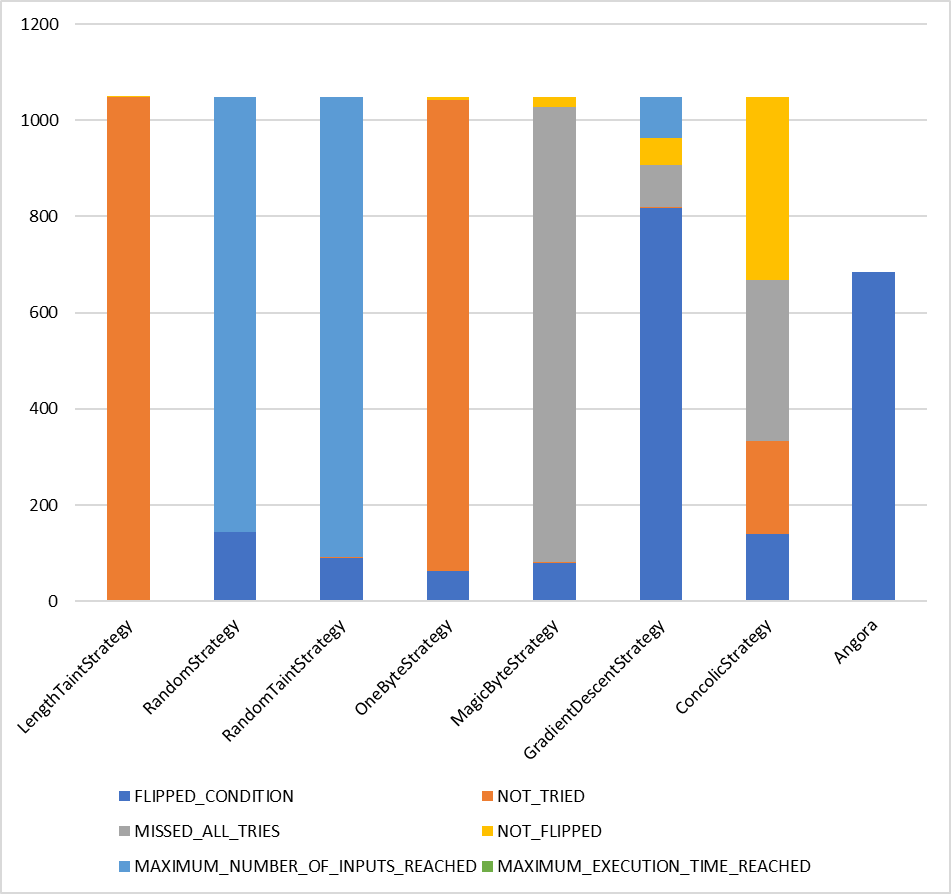
\includegraphics[width=.8\linewidth]{5_results/graphs/jhead-status.png}  
        \caption{Number of conditions flipped in the  \texttt{jhead} binary.}
        \label{fig:jheadStatus}
    \end{subfigure}
    \hfill
    \begin{subfigure}[b]{0.49\textwidth}
        \centering
        % include first image
        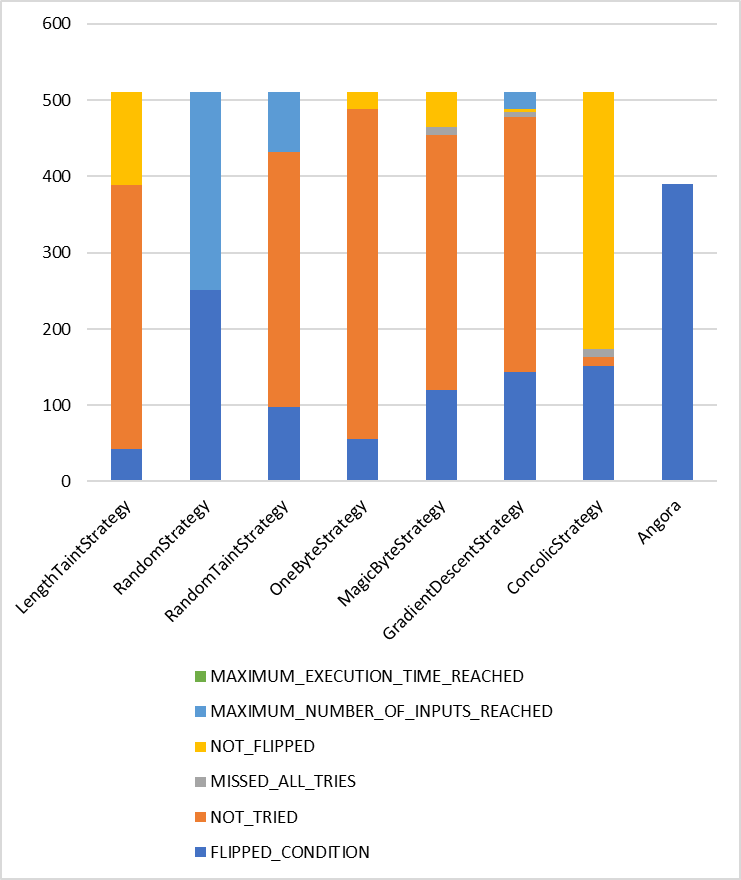
\includegraphics[width=.8\linewidth]{5_results/graphs/djpeg-status.png}  
        \caption{Number of conditions flipped in the  \texttt{djpeg} binary.}
        \label{fig:djpegStatus}
    \end{subfigure}
    \hfill
    \begin{subfigure}[b]{0.49\textwidth}
        \centering
        % include first image
        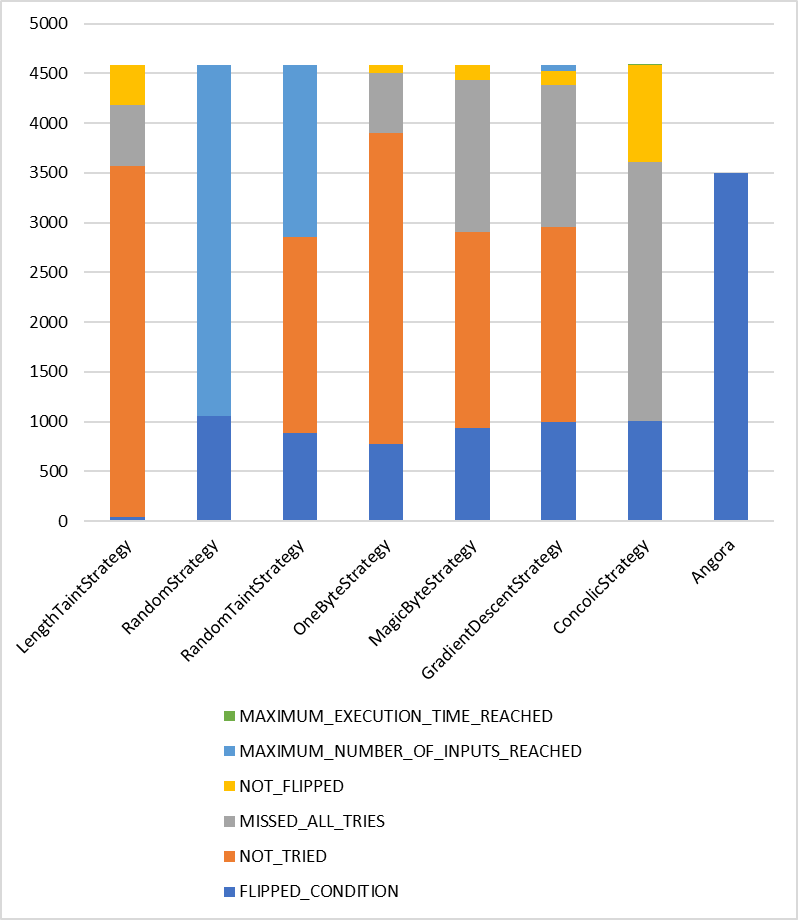
\includegraphics[width=.8\linewidth]{5_results/graphs/file-status.png}  
        \caption{Number of conditions flipped in the  \texttt{file} binary.}
        \label{fig:fileStatus}
    \end{subfigure}
    \hfill
    \begin{subfigure}[b]{0.49\textwidth}
        \centering
        % include first image
        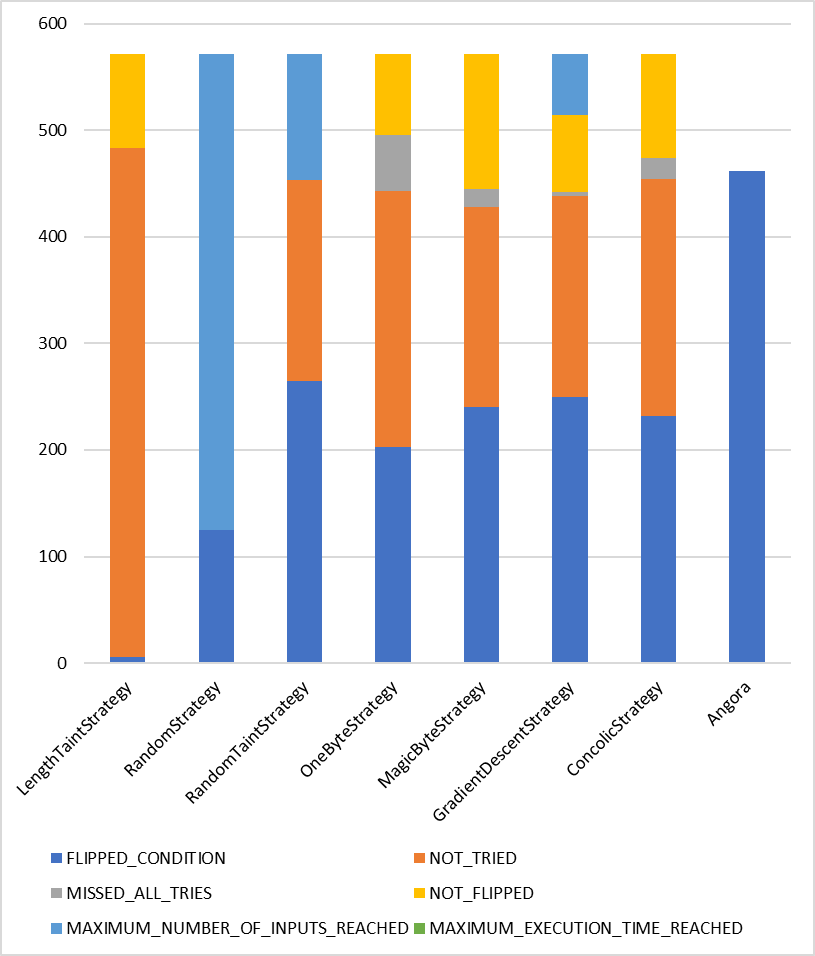
\includegraphics[width=.8\linewidth]{5_results/graphs/gif2png-status.png}  
        \caption{Number of conditions flipped in the  \texttt{gif2png} binary.}
        \label{fig:gif2pngStatus}
    \end{subfigure}
\caption{Number of conditions flipped per binary.}
\end{figure}

\begin{figure}[H]
    \centering
    \begin{subfigure}[b]{0.49\textwidth}
        \centering
        % include first image
        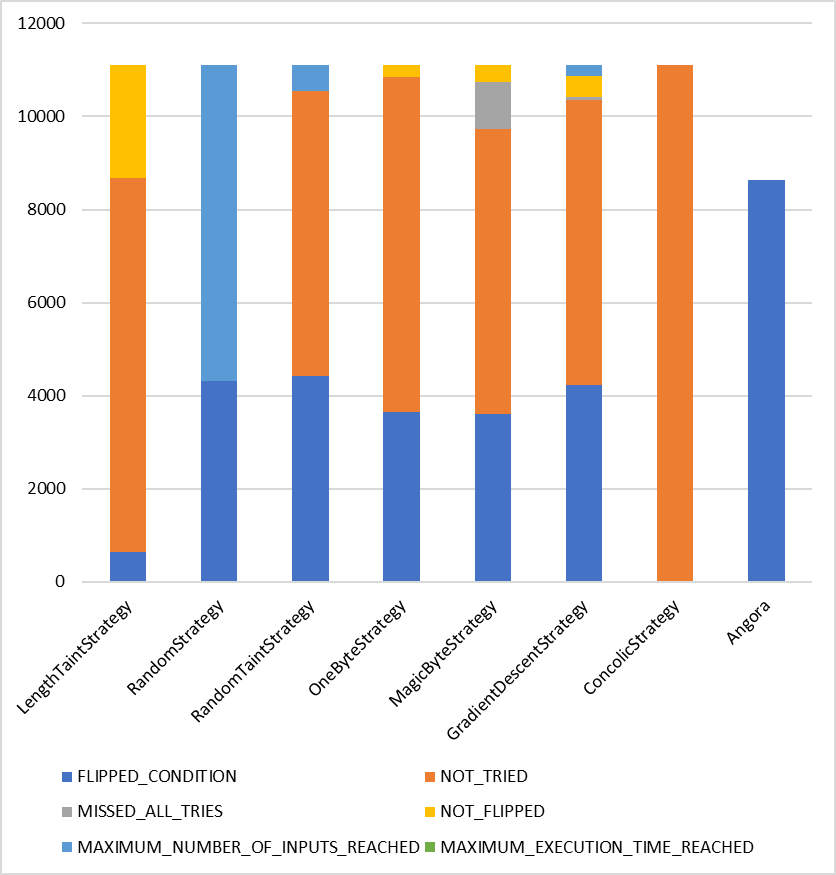
\includegraphics[width=.8\linewidth]{5_results/graphs/xmlwf-status.png}  
        \caption{Number of conditions flipped in the  \texttt{xmlwf} binary.}
        \label{fig:xmlwfStatus}
    \end{subfigure}
    \hfill
    \begin{subfigure}[b]{0.49\textwidth}
        \centering
        % include first image
        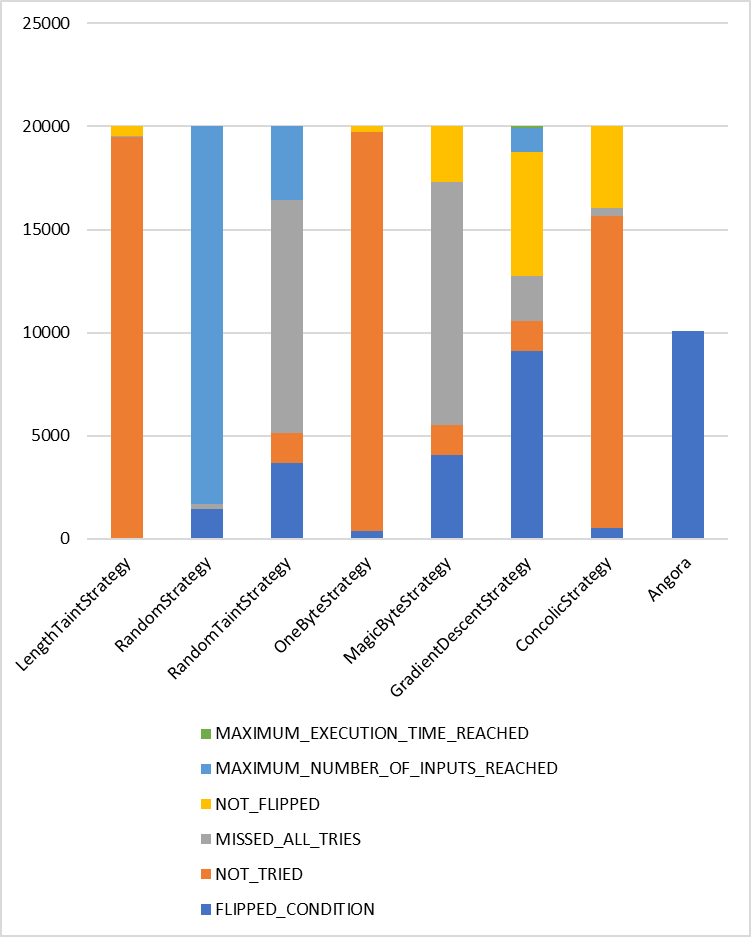
\includegraphics[width=.8\linewidth]{5_results/graphs/nm-status.png}  
        \caption{Number of conditions flipped in the \texttt{nm} binary.}
        \label{fig:nmStatus}
    \end{subfigure}
    \caption{Number of conditions flipped per binary.}
\end{figure}
When we compare the number of flips to the number of flips by Angora, we notice that only for the \texttt{jhead} program there are more flips found by our implemented strategies, than by Angora. This is mostly due to the flips found by the GradientDescent strategy, which outperforms all other strategies in this case as seen in Figure \ref{fig:djpegStatus}.

However, if we look at the \texttt{file} program, we see quite the opposite. We found only 30\% of all the flips found by Angora. And quite surprisingly the RandomStrategy, without any taint information, finds the most flips of all other strategies and the GradientDescent strategy finds nearly as many flips as the RandomTaintStrategy as seen in Figure \ref{fig:fileStatus}. 

This results seems to repeat itself in the \texttt{gif2png} program, where now the RandomTaintStrategy performs only better than the LengthTaintStrategy, but again there is little difference in total flips between the GradientDescentStrategy and the RandomTaintStrategy as seen in Figure \ref{fig:gif2pngStatus}.


In the \texttt{djpeg} program, again the RandomStrategy performs best, while now the Concolic and GradientDescent strategies compete for the second place as seen in Figure \ref{fig:djpegStatus}.

As seen in Figure \ref{fig:xmlwfStatus} \texttt{xmlwf} program, the RandomStrategy, RandomTaintStrategy and GradientDescent strategy perform about equally good, while the OneByte and MagicByte strategies are close for the second best strategy.

In the \texttt{nm} binary, as seen in Figure \ref{fig:nmStatus}, we see that the GradientDescent outperforms all other strategies, and we find a number of flips nearly equal to Angora.



\begin{figure}[H]
    \centering
    % include first image
    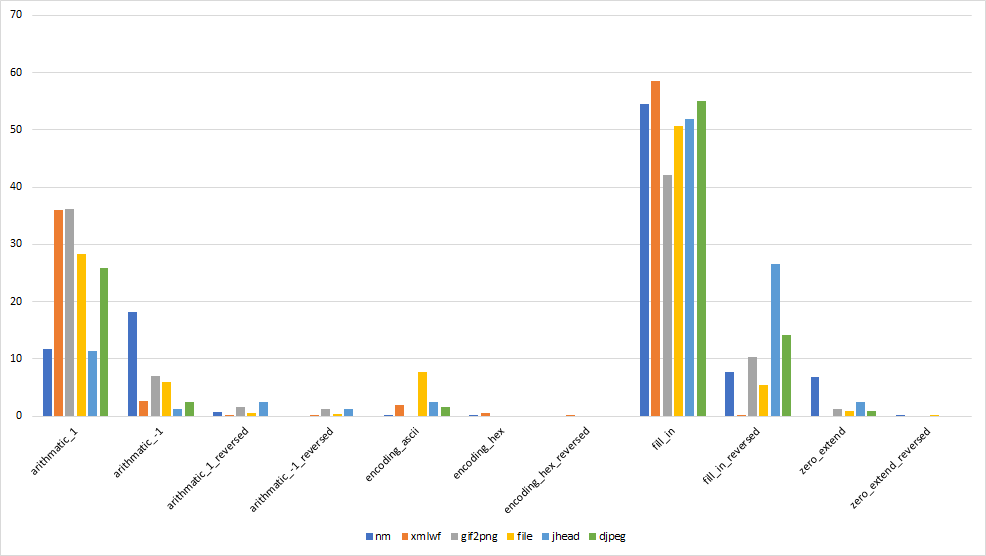
\includegraphics[width=.8\linewidth]{5_results/graphs/magic-byte-substrategy.png}  
    \caption{Number of flipped conditions using the MagicByte strategy per substrategy.}
    \label{fig:magicByteSubstrategies}
\end{figure}
We also made an overview of the substrategies used to flip a branch in the MagicByte strategy. We see clearly that filling in the magic bytes or using one-off values performs relatively well as substrategy. Also reversing a filled in value seems to work and converting the value to ASCII. We also see a difference between the programs which were checked. The \texttt{jhead} program seems to use more reversed statements, while the file program has more checks in ASCII values. The \texttt{nm} program has more flips by adding $-1$ to the value being compared.


\begin{figure}[H]
    \centering
    % include first image
    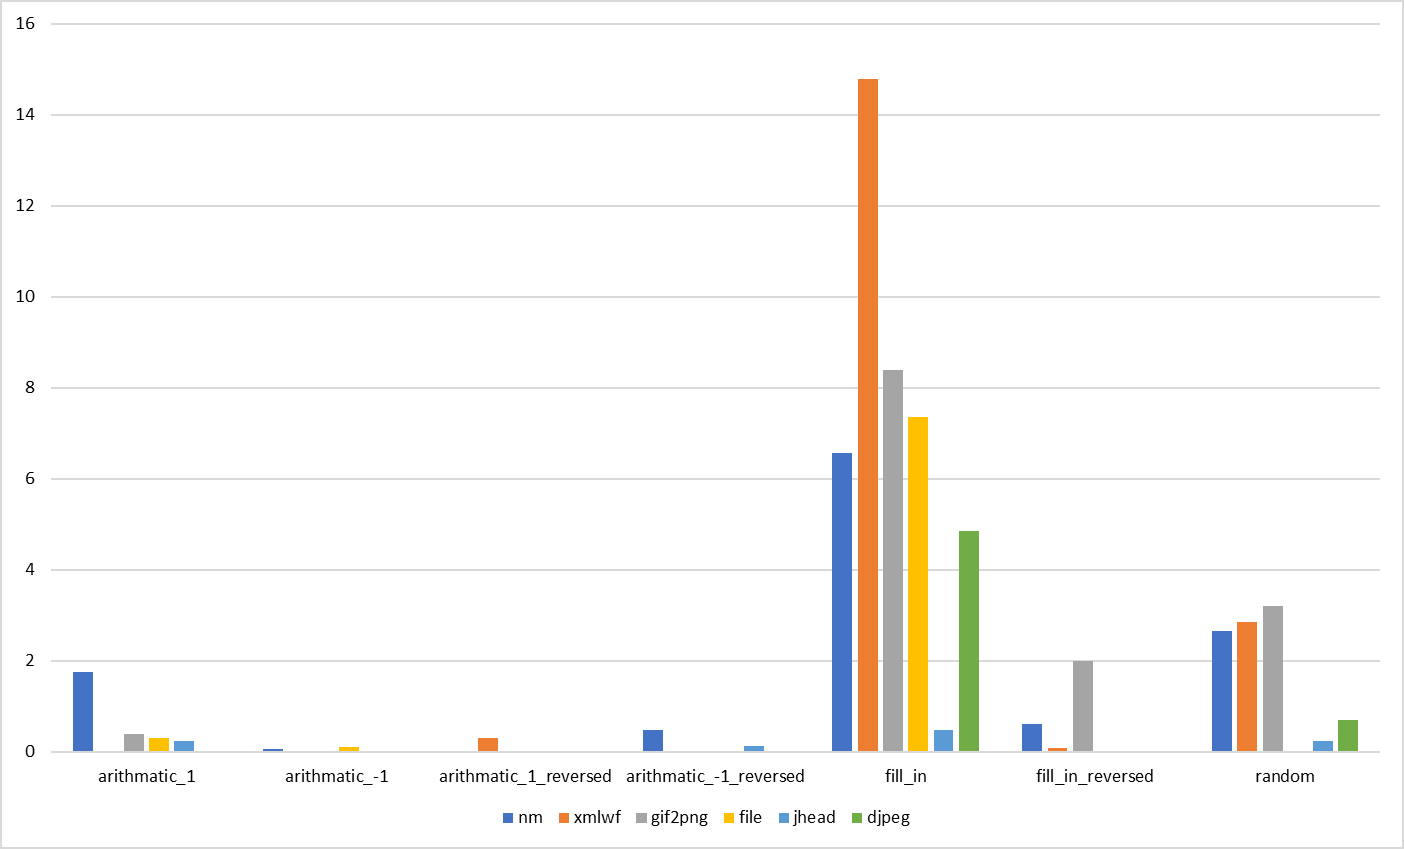
\includegraphics[width=.8\linewidth]{5_results/graphs/gradient-descent-substrategy.png}  
    \caption{Number of flipped conditions using the GradientDescent strategy per substrategy.}
    \label{fig:gradientDescentSubstrategies}
\end{figure}
We also made an overview of the substrategies used to flip a branch in the GradientDescent strategy. We see that it is most effective to use the value to be compared to in the \texttt{xmlwf} binary, however, most flips came from the initial value being compared.

From these graphs, we do not see a consistent result where one strategy outperform the another. We do see however, that the GradientDescent strategy works well in some cases like \texttt{jhead} and \texttt{nm} and that the RandomStrategy still finds a number of flips comparable to more sophisticated strategies.

From the comparison of the substrategies, we see that just filling in the bytes found in the comparison of a condition or doing this with one added or subtracted is a very effective way of flipping a condition, which supports the results from Redqueen \cite{aschermann2019redqueen}. 

From the comparison of the GradientDescent strategy, we see that combining this with the MagicByte strategy finds some new flips, so a combination of these strategies is a valid option as an improved GradientDescent strategy.


\section{Static Metrics}
In this section we will look at the results of the static metrics, namely the cyclomatic complexity, the Oviedo complexity, the chain size and the number of cases. An explanation of the metrics can be found in Section \ref{subsec:designStaticMetrics}. We assume that if we measure the same value from one of these metrics, the conditions have something in common. So we group all of these conditions together and we calculate the fraction of these which we flipped. For example, all conditions with an Oviedo complexity of 10 are grouped together and the fraction of flipped conditions is calculated. We do this for every metric.
We want to know if these metrics are correlated with the number of flips. To find such a relation, we use a correlation test. This can only be performed under the assumption that the values come from a normal distribution. 

We test if the correlation coefficient equals 0 as our null hypothesis with a confidence interval of 0.05. Our alternative hypothesis is that the correlation coefficient does not equal 0.

This test is done on the created pairs of conditions with the same value for the metric. For example, if there were only 2 possible values for the cyclomatic complexity, the sample size of the test equals 2. So even though we can have a lot of data which went into constructing the pairs, the number of unique values in the measurements influences the required correlation coefficient for a significant result.
We will give the correlation coefficient of all the metrics split by program, and a red background indicates a statistically significant result.
\todo{nrOfOffsets is dynamic, remove from table}


    \begin{table}[H]
    \centering
    \begin{tabular}{llllllll}
&  Ovie&Cycl&Offs&Cases&Chain&AbsD&RelD\\
GradientDescentStrategy&\cellcolor[HTML]{FFC7CE}{\color[HTML]{9C0006}0.0}&\cellcolor[HTML]{FFC7CE}{\color[HTML]{9C0006}0.0}&\cellcolor[HTML]{FFC7CE}{\color[HTML]{9C0006}0.0}&\cellcolor[HTML]{FFC7CE}{\color[HTML]{9C0006}0.01}&\cellcolor[HTML]{FFC7CE}{\color[HTML]{9C0006}0.02}&\cellcolor[HTML]{FFC7CE}{\color[HTML]{9C0006}0.05}&\cellcolor[HTML]{FFC7CE}{\color[HTML]{9C0006}0.0}\\
MagicByteStrategy&0.3&\cellcolor[HTML]{FFC7CE}{\color[HTML]{9C0006}0.01}&\cellcolor[HTML]{FFC7CE}{\color[HTML]{9C0006}0.0}&\cellcolor[HTML]{FFC7CE}{\color[HTML]{9C0006}0.0}&\cellcolor[HTML]{FFC7CE}{\color[HTML]{9C0006}0.0}&\cellcolor[HTML]{FFC7CE}{\color[HTML]{9C0006}0.0}&0.15\\
OneByteStrategy&0.34&\cellcolor[HTML]{FFC7CE}{\color[HTML]{9C0006}0.0}&\cellcolor[HTML]{FFC7CE}{\color[HTML]{9C0006}0.0}&\cellcolor[HTML]{FFC7CE}{\color[HTML]{9C0006}0.0}&\cellcolor[HTML]{FFC7CE}{\color[HTML]{9C0006}0.0}&\cellcolor[HTML]{FFC7CE}{\color[HTML]{9C0006}0.0}&\cellcolor[HTML]{FFC7CE}{\color[HTML]{9C0006}0.0}\\
LengthTaintStrategy&nan&nan&nan&nan&nan&nan&nan\\
ConcolicStrategy&\cellcolor[HTML]{FFC7CE}{\color[HTML]{9C0006}0.0}&\cellcolor[HTML]{FFC7CE}{\color[HTML]{9C0006}0.0}&0.11&\cellcolor[HTML]{FFC7CE}{\color[HTML]{9C0006}0.0}&\cellcolor[HTML]{FFC7CE}{\color[HTML]{9C0006}0.0}&0.41&0.12\\
RandomStrategy&0.22&0.2&0.12&\cellcolor[HTML]{FFC7CE}{\color[HTML]{9C0006}0.0}&\cellcolor[HTML]{FFC7CE}{\color[HTML]{9C0006}0.0}&\cellcolor[HTML]{FFC7CE}{\color[HTML]{9C0006}0.0}&0.05\\
RandomTaintStrategy&0.08&\cellcolor[HTML]{FFC7CE}{\color[HTML]{9C0006}0.0}&\cellcolor[HTML]{FFC7CE}{\color[HTML]{9C0006}0.0}&\cellcolor[HTML]{FFC7CE}{\color[HTML]{9C0006}0.0}&\cellcolor[HTML]{FFC7CE}{\color[HTML]{9C0006}0.0}&\cellcolor[HTML]{FFC7CE}{\color[HTML]{9C0006}0.0}&0.08\\

    \end{tabular}
    \caption{Significant difference of several metrics \texttt{jhead} binary}
    \label{tab:jheadWhitneyU}
    \end{table}
    
    
    
In Table \ref{tab:jheadCor}, the LengthTaintStrategy found no flips, hence the correlation coefficient was 0 everywhere.

\begin{table}[H]
    \centering
    \begin{tabular}{llllll}
\textbf{Correlation   coefficient} & nrOfOffsets & Cyclomatic & Oviedo   & Chain size & Cases    \\
GradientDescentStrategy            & 0,205318    & 0,011416   & 0,011457 & 0,21239     & -0,93573 \\
ConcolicStrategy                   & 0,631473    & -0,00485   & 0,000411 & 0,249513    & -0,74595 \\
MagicByteStrategy                  & 0,738903    & -0,03474   & -0,03581 & 0,099961    & -0,88598 \\
RandomStrategy                     & 0,745772    & 0,287292   & 0,26743  & 0,256173    & -0,88548 \\
RandomTaintStrategy                & -0,2137     & -0,02883   & -0,03515 & -0,03184    & -0,64501 \\
LengthTaintStrategy                & -0,44039    & 0,221465   & 0,253842 & 0,119641    & -0,5309  \\
OneByteStrategy                    & -0,33029    & -0,09256   & -0,10361 & -0,06478    & -0,56449 \\hline
Sample size                        & 4           & 10         & 11       & 32          & 3       
\end{tabular}
    \caption{Correlation coefficients of the \texttt{djpeg} binary}
    \label{tab:djpegCor}
\end{table}
\begin{table}[H]
    \centering
    \begin{tabular}{llllll}
\textbf{Correlation   coefficient} & nrOfOffsets & Cyclomatic & Oviedo   & Chain size                                            & Cases                                                   \\
GradientDescentStrategy            & -0,23907    & 0,113457   & 0,195891 & -0,24598                                               & \cellcolor[HTML]{FFC7CE}{\color[HTML]{9C0006} 0,731024} \\
ConcolicStrategy                   & -0,21984    & 0,069807   & 0,130543 & -0,2832                                                & 0,669845                                                \\
MagicByteStrategy                  & -0,21204    & 0,136656   & 0,200582 & -0,24097                                               & 0,66458                                                 \\
RandomStrategy                     & -0,27992    & 0,015236   & 0,119628 & \cellcolor[HTML]{FFC7CE}{\color[HTML]{9C0006} -0,3187} & 0,682533                                                \\
RandomTaintStrategy                & -0,18134    & 0,07412    & 0,173287 & -0,23057                                               & 0,680243                                                \\
LengthTaintStrategy                & -0,11651    & 0,299711   & 0,097546 & 0,14474                                                & -0,59245                                                \\
OneByteStrategy                    & -0,1145     & 0,016899   & 0,055826 & -0,21049                                               & 0,664689                                                \\hline
Sample size                        & 23          & 32         & 46       & 47                                                     & 8                                                      
\end{tabular}
    \caption{Correlation coefficients of the \texttt{file} binary}
    \label{tab:fileCor}
\end{table}
\begin{table}[H]
    \centering
   \begin{tabular}{llllll}
\textbf{Correlation   coefficient} & nrOfOffsets & Cyclomatic                                              & Oviedo                                                  & Chain size & Cases \\
GradientDescentStrategy            & -0,48226    & \cellcolor[HTML]{FFC7CE}{\color[HTML]{9C0006} 0,747139} & \cellcolor[HTML]{FFC7CE}{\color[HTML]{9C0006} 0,808394} & -0,06959    &       \\
ConcolicStrategy                   & -0,4523     & 0,573681                                                & 0,605348                                                & -0,06253    &       \\
MagicByteStrategy                  & -0,45436    & \cellcolor[HTML]{FFC7CE}{\color[HTML]{9C0006} 0,775257} & \cellcolor[HTML]{FFC7CE}{\color[HTML]{9C0006} 0,799827} & -0,25979    &       \\
RandomStrategy                     & 0,095591    & 0,563317                                                & 0,550047                                                & -0,26082    &       \\
RandomTaintStrategy                & -0,10081    & 0,597975                                                & 0,558925                                                & 0,270854    &       \\
LengthTaintStrategy                & -0,41188    & 0,589697                                                & 0,49245                                                 & -0,20071    &       \\
OneByteStrategy                    & 0,104705    & 0,631743                                                & 0,550275                                                & 0,029647    &       \\hline
Sample size                        & 7           & 8                                                       & 8                                                       & 11          & 2    
\end{tabular}
    \caption{Correlation coefficients of the \texttt{gif2png} binary}
    \label{tab:gif2pngCor}
\end{table}
In Table \ref{tab:gif2pngCor} there were only 2 possible values for the number of cases, hence the correlation coefficient could not be calculated.

\begin{table}[H]
    \centering
    \begin{tabular}{llllll}
\textbf{Correlation   coefficient} & nrOfOffsets                                             & Cyclomatic                                             & Oviedo                                                  & Chain size & Cases    \\
GradientDescentStrategy            & \cellcolor[HTML]{FFC7CE}{\color[HTML]{9C0006} 0,55746}  & -0,19821                                               & -0,22831                                                & 0,030608    & 0,402348 \\
ConcolicStrategy                   &                                                         &                                                        &                                                         &             &          \\
MagicByteStrategy                  & \cellcolor[HTML]{FFC7CE}{\color[HTML]{9C0006} -0,43595} & -0,17436                                               & -0,2191                                                 & -0,01083    & 0,433612 \\
RandomStrategy                     & \cellcolor[HTML]{FFC7CE}{\color[HTML]{9C0006} 0,497585} & 0,162392                                               & 0,174867                                                & 0,08793     & 0,391188 \\
RandomTaintStrategy                & \cellcolor[HTML]{FFC7CE}{\color[HTML]{9C0006} -0,5751}  & -0,16767                                               & -0,19832                                                & 0,069683    & 0,386711 \\
LengthTaintStrategy                & -0,19668                                                & \cellcolor[HTML]{FFC7CE}{\color[HTML]{9C0006} 0,45029} & \cellcolor[HTML]{FFC7CE}{\color[HTML]{9C0006} 0,461258} & 0,003246    & -0,36074 \\
OneByteStrategy                    & -0,19313                                                & -0,17576                                               & -0,21887                                                & 0,026968    & 0,397983 \\hline
Sample size                        & 38                                                      & 36                                                     & 53                                                      & 53          & 18      
\end{tabular}
    \caption{Correlation coefficients of the \texttt{xmlwf} binary}
    \label{tab:xmlwfCor}
\end{table}
\begin{table}[H]
    \centering
    \begin{tabular}{llllll}
\textbf{Correlation   coefficient} & nrOfOffsets                                             & Cyclomatic & Oviedo   & Chain size                                             & Cases    \\
GradientDescentStrategy            & -0,00653                                                & 0,159567   & 0,195467 & \cellcolor[HTML]{FFC7CE}{\color[HTML]{9C0006} -0,43679} & -0,60323 \\
ConcolicStrategy                   & 0,214441                                                & -0,10202   & 0,02986  & -0,01512                                                & -0,28962 \\
MagicByteStrategy                  & \cellcolor[HTML]{FFC7CE}{\color[HTML]{9C0006} -0,43907} & 0,228513   & 0,189986 & 0,195629                                                & -0,45239 \\
RandomStrategy                     & 0,158416                                                & -0,07771   & 0,009494 & \cellcolor[HTML]{FFC7CE}{\color[HTML]{9C0006} -0,3671}  & -0,11419 \\
RandomTaintStrategy                & \cellcolor[HTML]{FFC7CE}{\color[HTML]{9C0006} -0,37221} & 0,265475   & 0,178601 & -0,3011                                                 & -0,44465 \\
LengthTaintStrategy                & -0,22297                                                & 0,122727   & 0,052122 & -0,17033                                                & -0,38742 \\
OneByteStrategy                    & -0,21442                                                & 0,212724   & 0,217546 & -0,16366                                                & -0,32016 \\hline
Sample size                        & 51                                                      & 40         & 65       & 38                                                      & 6       
\end{tabular}
    \caption{Correlation coefficients of the \texttt{nm} binary}
    \label{tab:nmCor}
\end{table}

From these results, we see that no metric gave a consistent correlation with the number of flips in any binary with any strategy. The chain size gave 7 statistically significant results out of the 42 tests, however 3 of those occurred in the \texttt{xmlwf} binary, so we do not consider this enough to conclude something from this metric.
Unfortunately, it looks as if the chosen static metrics do not give enough insight in the conditions to relate directly with the performance of a strategy. In the next section we will try to find a relation with the dynamic metrics.

\section{Dynamic metrics}
In this section we will look at the results of each strategy per binary in terms of depth, number of tainted bytes present in the condition, and time spend calculating the inputs. 
As we have seen in the overall results, often the RandomStrategy outperforms more sophisticated strategies. We hope to find a reason why this is by looking at these statistics more closely. 
In order to say something about the effectiveness of a strategy, we look at the time spend on a strategy. 

\subsection{Depth}
In this section we will look at the absolute depth of the conditions flipped per strategy and the relative depth of the conditions flipped per strategy.
\paragraph{Absolute depth}
We will first look at the absolute depth. We look the longest trace as 100\% of the length, and placed the other conditions in ranges of 10\% based on this total.
The totals on which the percentages were calculated can be found in Appendix \ref{appendix:depth}. Since we exclude conditions which we have already seen, we notice that the distribution of unique conditions per bucket is not uniform. In the \texttt{nm} binary, nearly all unique conditions which are seen are present in the first bucket, while the last bucket only has 12 unique conditions, while the \texttt{djpeg} binary has a peak of unique conditions at the 50-70\% bucket while in the 10-20\% bucket there is not a single unique condition.
\begin{figure}[H]
    \centering
    % include first image
    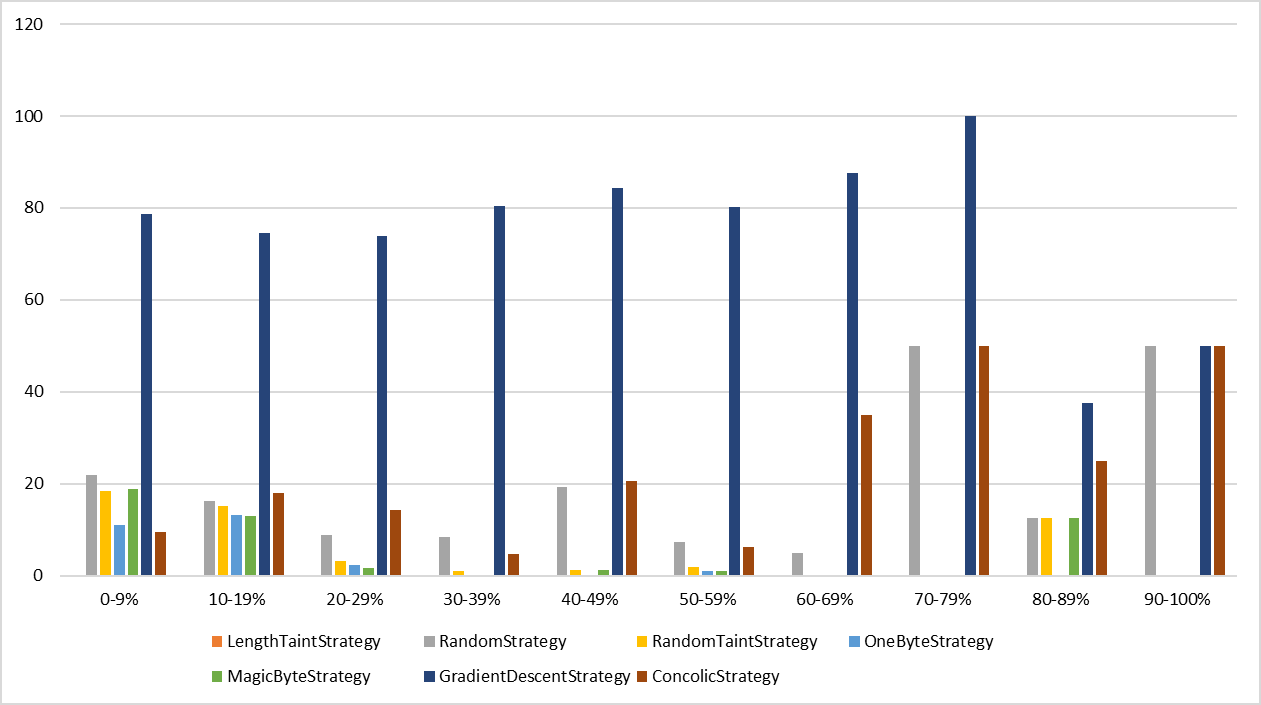
\includegraphics[width=.8\linewidth]{5_results/graphs/jhead-depth.png}  
    \caption{Percentage of flips per depth in the \texttt{jhead} binary.}
    \label{fig:jheadDepth}
\end{figure}
We see  in Figure \ref{fig:jheadDepth} that the GradientDescent strategy outperforms the other strategies at nearly every depth. We also see that the RandomStrategy seems to be on par, or sometimes better than the ConcolicStrategy per depth.
\begin{figure}[H]
    \centering
    % include first image
    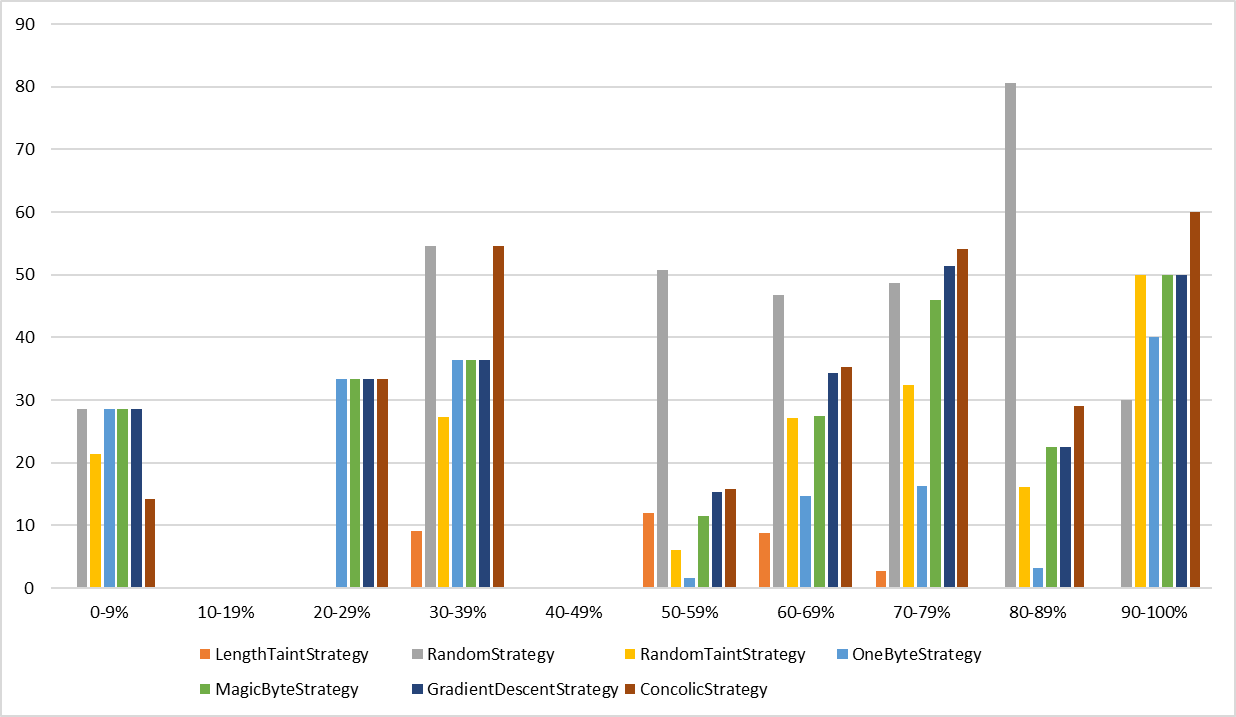
\includegraphics[width=.8\linewidth]{5_results/graphs/djpeg-depth.png}  
    \caption{Percentage of flips per depth in the \texttt{djpeg} binary.}
    \label{fig:djpegDepth}
\end{figure}
In Figure \ref{fig:djpegDepth} we see that the ConcolicStrategy seems to perform pretty good deeper in the program. An unexpected result is that the RandomStrategy seems to be out performing the other strategies in the 80-90\% bucket.
\begin{figure}[H]
    \centering
    % include first image
    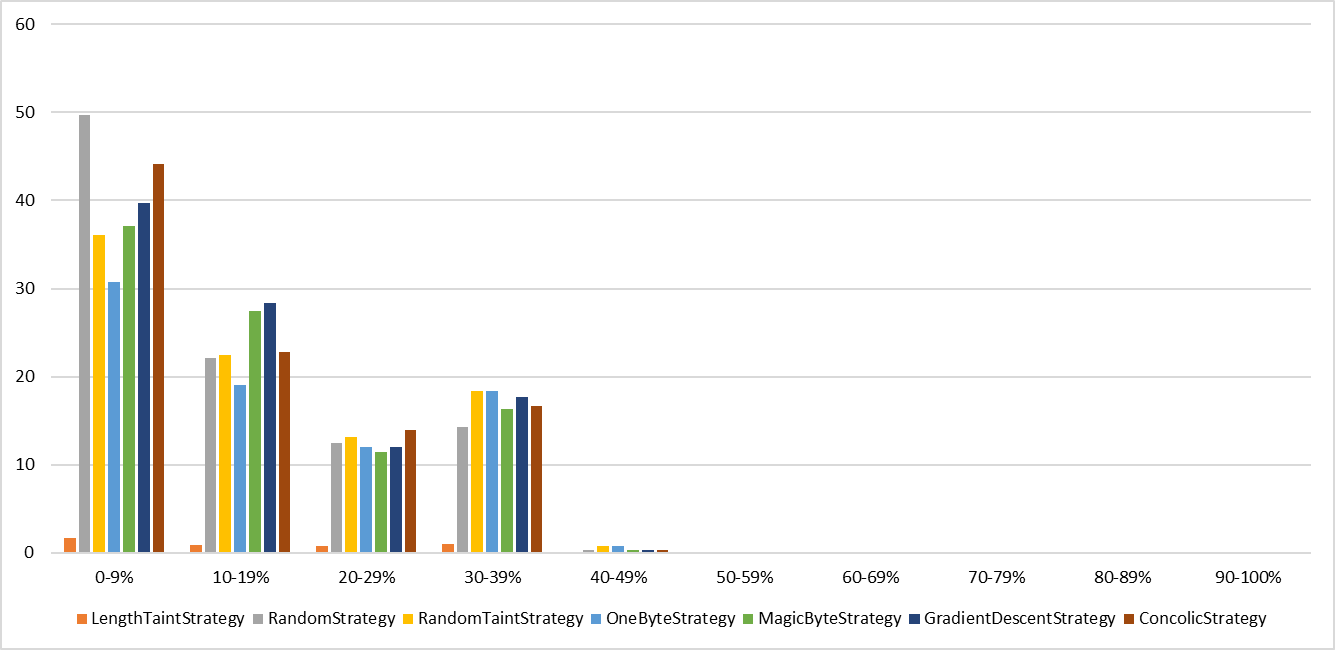
\includegraphics[width=.8\linewidth]{5_results/graphs/file-depth.png}  
    \caption{Percentage of flips per depth in the \texttt{file} binary.}
    \label{fig:fileDepth}
\end{figure}
In the \texttt{file} binary, we see that the metric we used for depth might be sensitive to outliers in Figure \ref{fig:fileDepth}. We will discuss this metric in depth in Chapter \ref{chap:discussion}, but it seems that if there has been 1 long trace, most shorter traces fall in the earlier buckets. In these buckets, we see in the first bucket a large impact of the RandomStrategy, which decreases when the depth decreases, but in the 30-40\% bucket, the number of flips seems to increase followed by a quick decrease in the number of flipped conditions. We checked if this could have something to do with losing taint information, but this was not the case.
\begin{figure}[H]
    \centering
    % include first image
    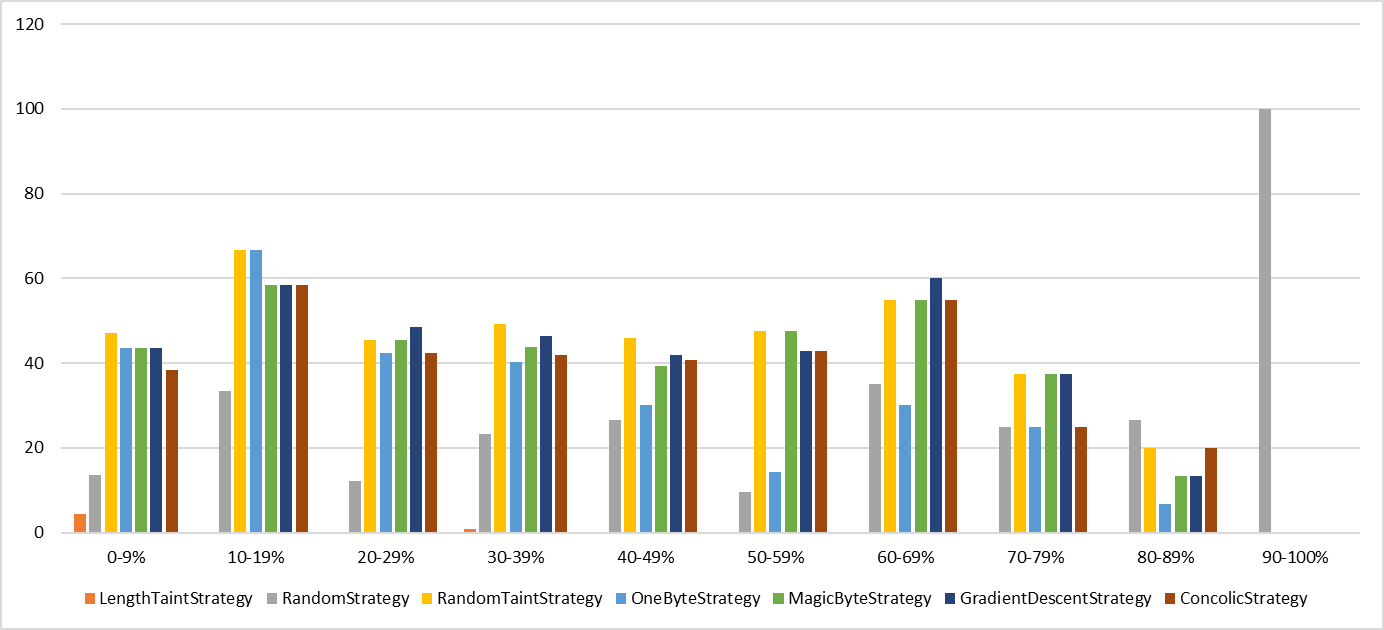
\includegraphics[width=.8\linewidth]{5_results/graphs/gif2png-depth.png}  
    \caption{Percentage of flips per depth in the \texttt{gif2png} binary.}
    \label{fig:gif2pngDepth}
\end{figure}
When we look at the depth of the results of the percentage of flips of the \texttt{gif2png} binary in Figure \ref{fig:gif2pngDepth}, we notice that most strategies perform equally well per depth, but in the final bucket only the RandomStrategy manages to flip conditions. There were only 4 conditions flipped in this last bucket, which were all flipped by this strategy, so this might skew with the results, again we will discuss this metric in Chapter \ref{chap:discussion}.
\begin{figure}[H]
    \centering
    % include first image
    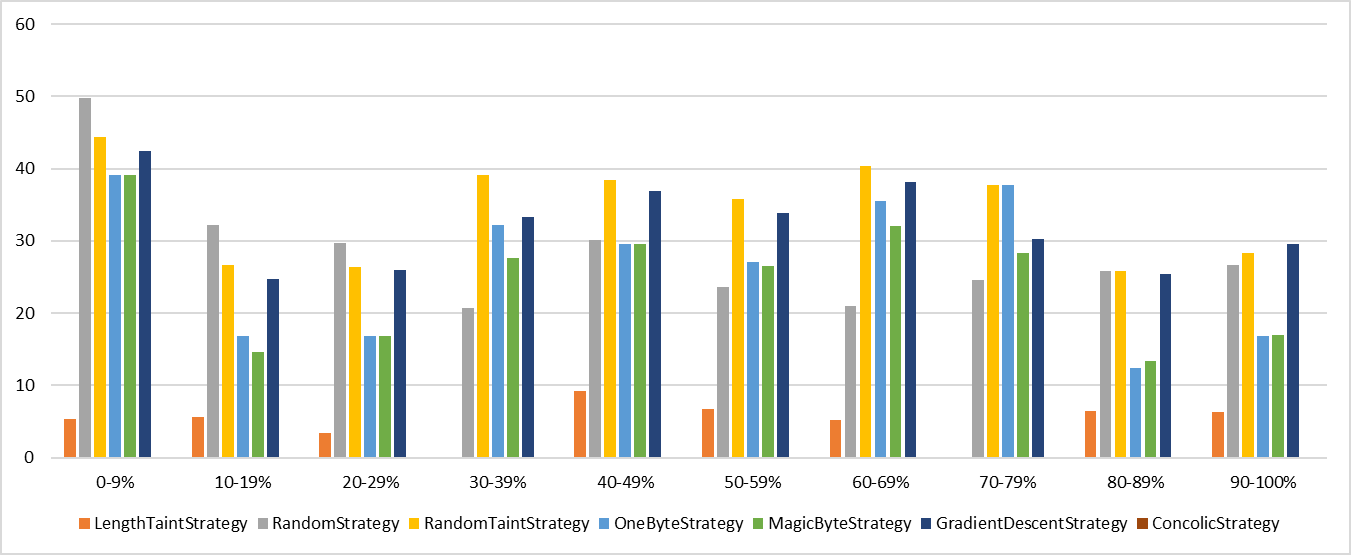
\includegraphics[width=.8\linewidth]{5_results/graphs/xmlwf-depth.png}  
    \caption{Percentage of flips per depth in the \texttt{xmlwf} binary.}
    \label{fig:xmlwfDepth}
\end{figure}
The \texttt{xmlwf} binary has a pretty even distribution of the number of flips. This could be attributed to the structure of the program, which checks if something is a valid XML file. If this is done recursively, the same strategies could mutate the elements of the xml in somewhat the same way. We see that the RandomTaint strategy performs better or better than the GradientDescent strategy.
\begin{figure}[H]
    \centering
    % include first image
    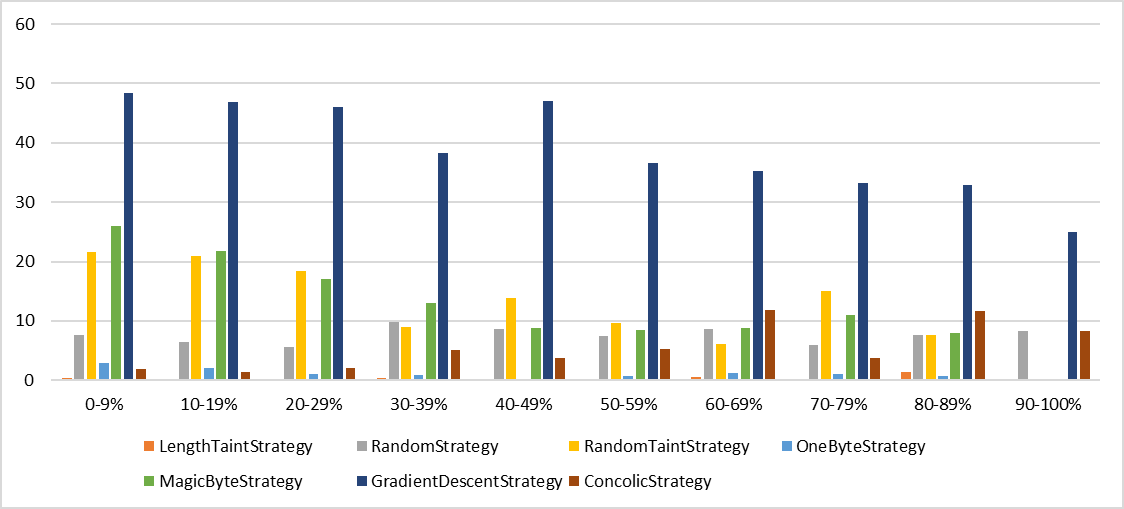
\includegraphics[width=.8\linewidth]{5_results/graphs/nm-depth.png}  
    \caption{Percentage of flips per depth in the \texttt{nm} binary.}
    \label{fig:nmDepth}
\end{figure}
In the \texttt{nm} binary, we see that the GradientDescent strategy outperforms nearly all other strategies with nearly twice as many flipped conditions than all others. We also see the ConcolicStrategy increasing if we are deeper in the program.

We again see that fr the \texttt{nm} and \texttt{jhead} programs the GradientDescent strategy works best, but for other programs this differs. Also the ConcolicStrategy works better deeper in the program, which is an expected result. However, for some programs like \texttt{djpeg} the RandomStrategy performs better than expected on multiple depths. Further research is required to see why this happens for this program.

\paragraph{Relative depth}
We also looked at the depth of a condition in a trace, and we placed all these conditions in buckets of 10\% based on their position in the corresponding trace.
\begin{figure}[H]
    \centering
    % include first image
    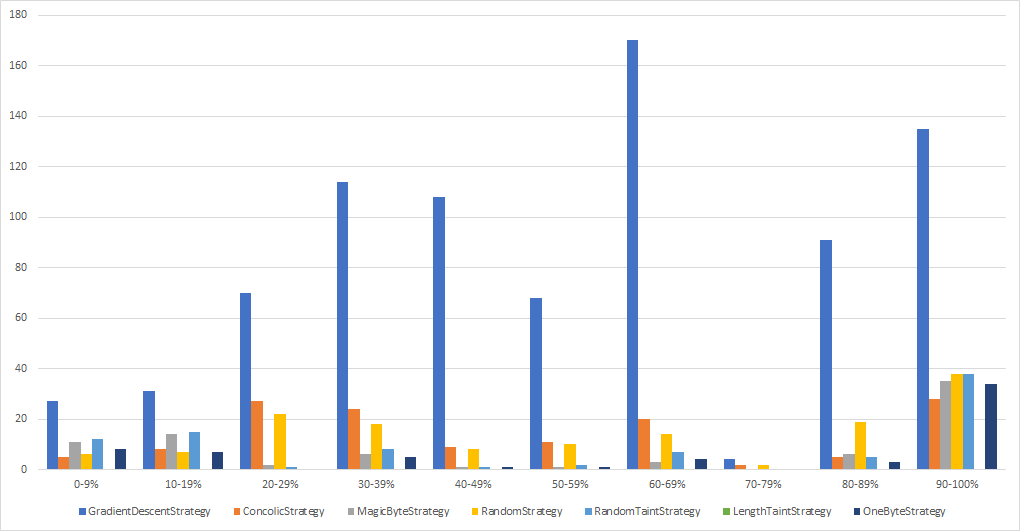
\includegraphics[width=.8\linewidth]{5_results/graphs/jhead-depth-relative.png}  
    \caption{Percentage of flips per relative depth in the \texttt{jhead} binary.}
    \label{fig:jheadDepthRelative}
\end{figure}
When we look at the performance of the GradientDescentStrategy in Figure \ref{fig:jheadDepthRelative}, we see that it outperforms most other strategies. It is interesting to note that the number of flips is not uniform in the trace, at the \texttt{70-79\%} bucket, there are hardly any flips found.

\begin{figure}[H]
    \centering
    % include first image
    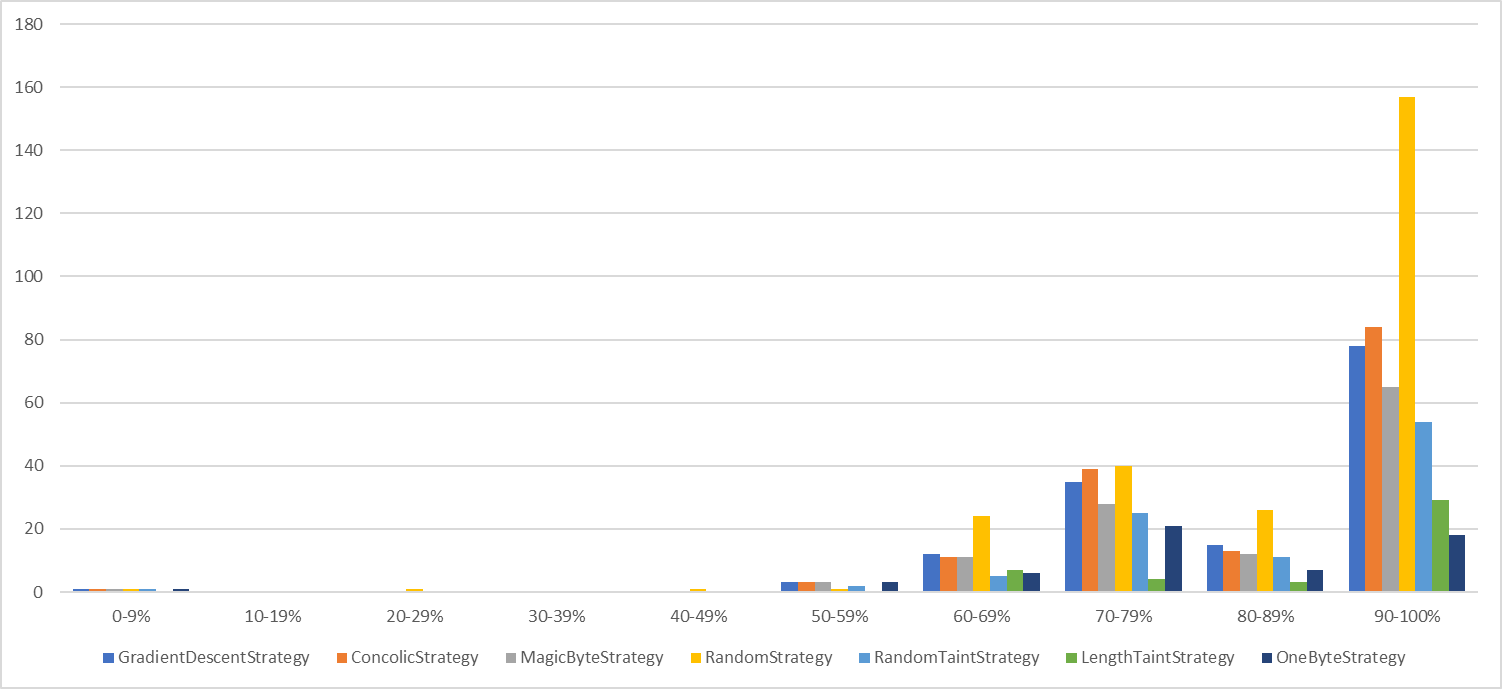
\includegraphics[width=.8\linewidth]{5_results/graphs/djpeg-depth-relative.png}  
    \caption{Percentage of flips per relative depth in the \texttt{djpeg} binary.}
    \label{fig:djpegDepthRelative}
\end{figure}
In Figure \ref{fig:jheadDepthRelative}, it appears as if the entire first \texttt{50\%} of the program has very little flips, and only at the end of the program do there appear to be flips, where the RandomStrategy outperforms the other strategies.


\begin{figure}[H]
    \centering
    % include first image
    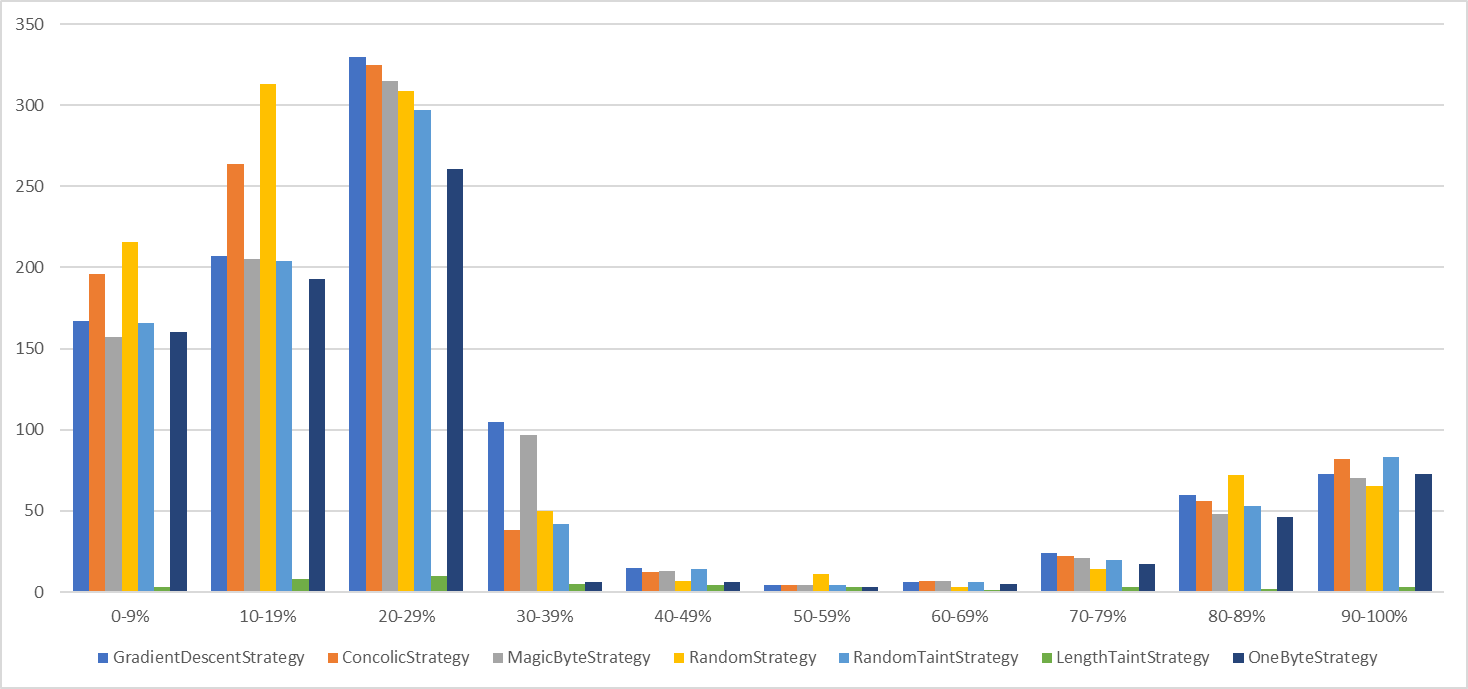
\includegraphics[width=.8\linewidth]{5_results/graphs/file-depth-relative.png}  
    \caption{Percentage of flips per relative depth in the \texttt{file} binary.}
    \label{fig:fileDepthRelative}
\end{figure}
It is interesting to see that with the relative depth we get a better sense of where in the traces the flips occur. In Figure \ref{fig:fileDepthRelative}, we see that in the first \texttt{30\%} buckets most flips of the program occur, then a decrease in the number of flips and then towards the end again more flips.

\begin{figure}[H]
    \centering
    % include first image
    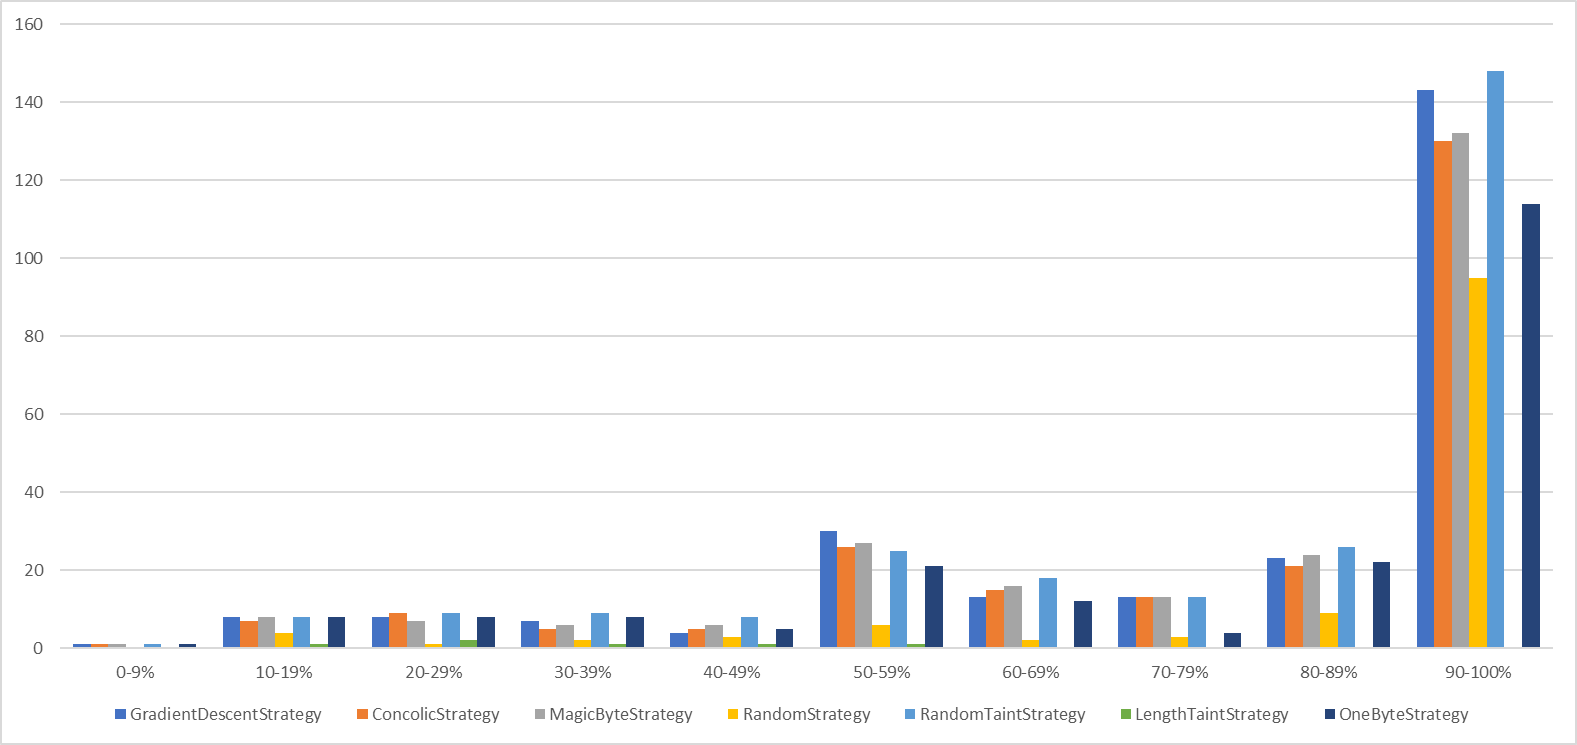
\includegraphics[width=.8\linewidth]{5_results/graphs/gif2png-depth-relative.png}  
    \caption{Percentage of flips per relative depth in the \texttt{gif2png} binary.}
    \label{fig:gif2pngDepthRelative}
\end{figure}
In the relative depth of the \texttt{gif2png} binary in Figure \ref{fig:gif2pngDepthRelative}, we notice that most flips occur in the last part of the traces, while there are hardly any flips in the first part of the program.

\todo{xmlwf is missing}

\begin{figure}[H]
    \centering
    % include first image
    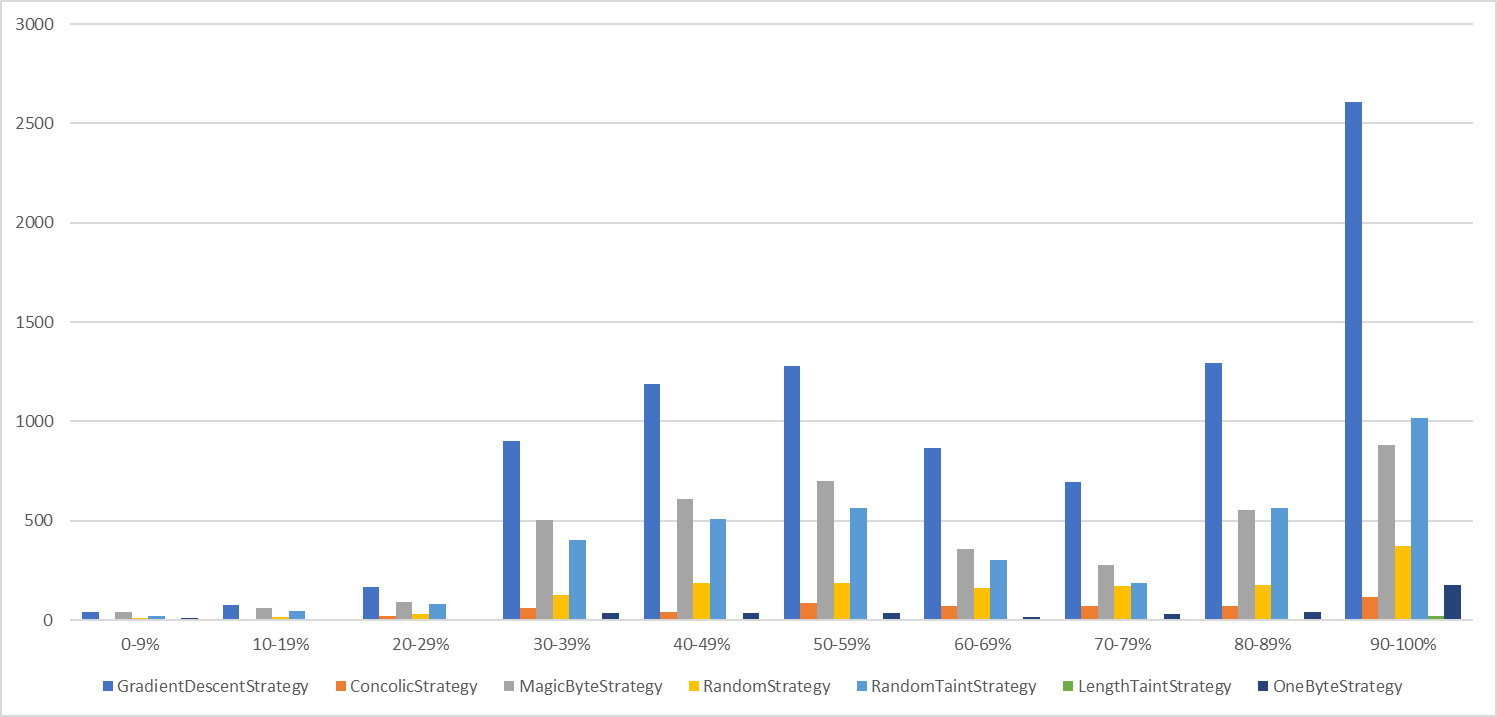
\includegraphics[width=.8\linewidth]{5_results/graphs/nm-depth-relative.png}  
    \caption{Percentage of flips per relative depth in the \texttt{nm} binary.}
    \label{fig:nmDepthRelative}
\end{figure}
In Figure \ref{fig:nmDepthRelative}, we see that the GradientDescentStrategy outperforms most other strategies, especially in the last bucket of the traces.

\subsection{Offsets}
In this subsection we will look at the results of the comparison of the strategies in binaries when looking at the number of offsets present in a condition. We take the total number of conditions per offset as 100\% and look at the relative performance of each strategy. The totals on which the percentages were calculated can be found in Appendix \ref{appendix:offsets}.
\begin{figure}[H]
    \centering
    % include first image
    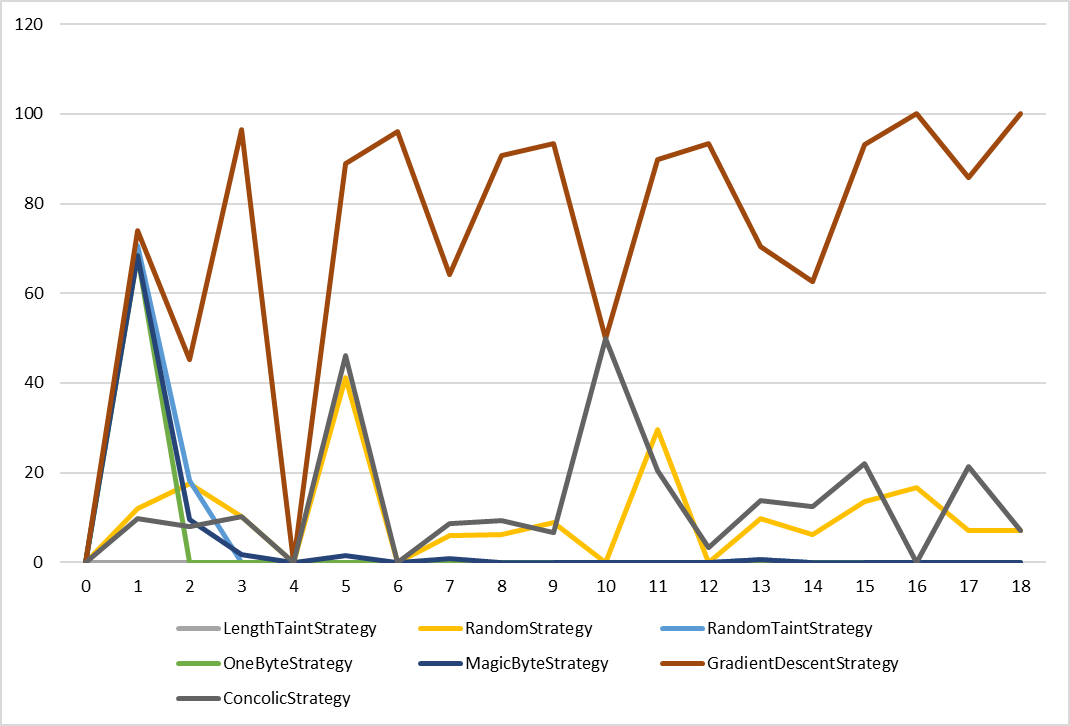
\includegraphics[width=.8\linewidth]{5_results/graphs/jhead-offsets.png}  
    \caption{Percentage of conditions flipped per number of offsets present from the input in the \texttt{jhead} binary.}
    \label{fig:jheadOffsets}
\end{figure}
We see some interesting behaviour of the GradientDescent strategy in Figure \ref{fig:jheadOffsets}, which outperforms all other strategies for every number of offsets present. We also see that the Concolic and Random stragies still find flips when more offsets are present in the condition. Most strategies find flips when only 1 offset from the input is present.
\begin{figure}[H]
    \centering
    % include first image
    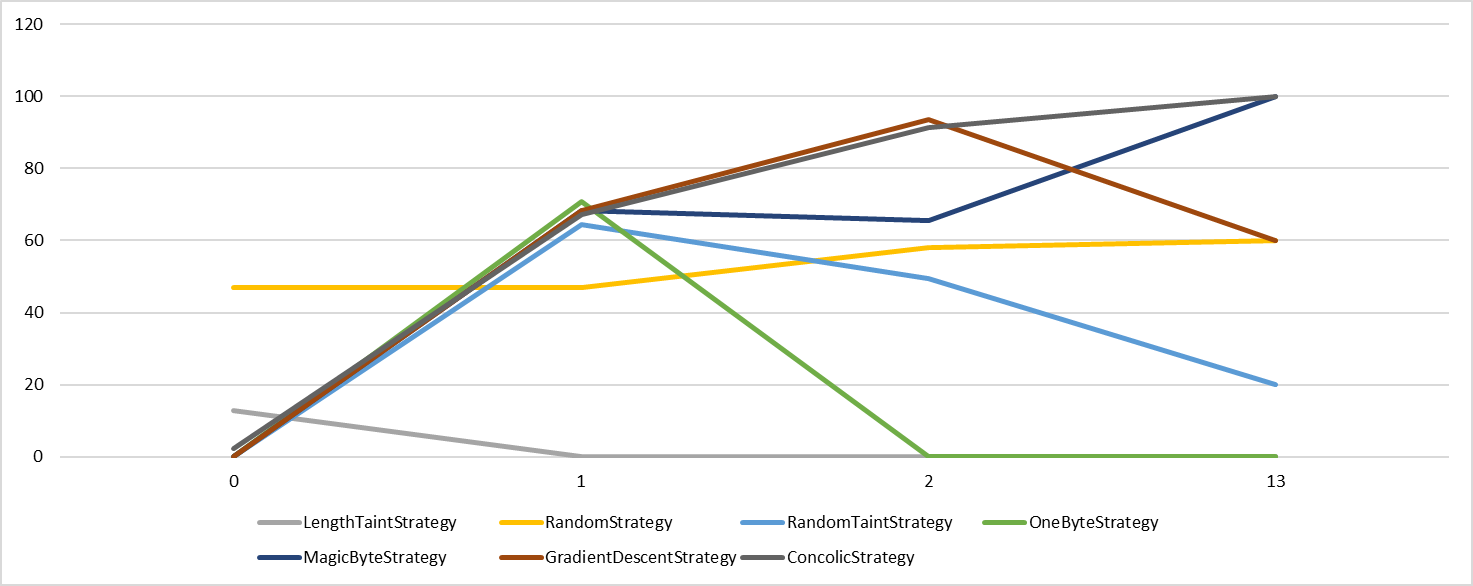
\includegraphics[width=.8\linewidth]{5_results/graphs/djpeg-offsets.png}  
    \caption{Percentage of conditions flipped per number of offsets present from the input in the \texttt{djpeg} binary.}
    \label{fig:djpegOffsets}
\end{figure}
Again we see that most strategies find flips with 1 offset in Figure \ref{fig:djpegOffsets}. What is interesting, is that the RandomStrategy seems to find way more flips when no offsets are present than the other strategies. After this, it is outperformed by other strategies. However, this might indicate that some taint has been lost during the execution of the \texttt{djpeg} runs, since here the input influences the conditions, while no offsets from the input were found.
\begin{figure}[H]
    \centering
    % include first image
    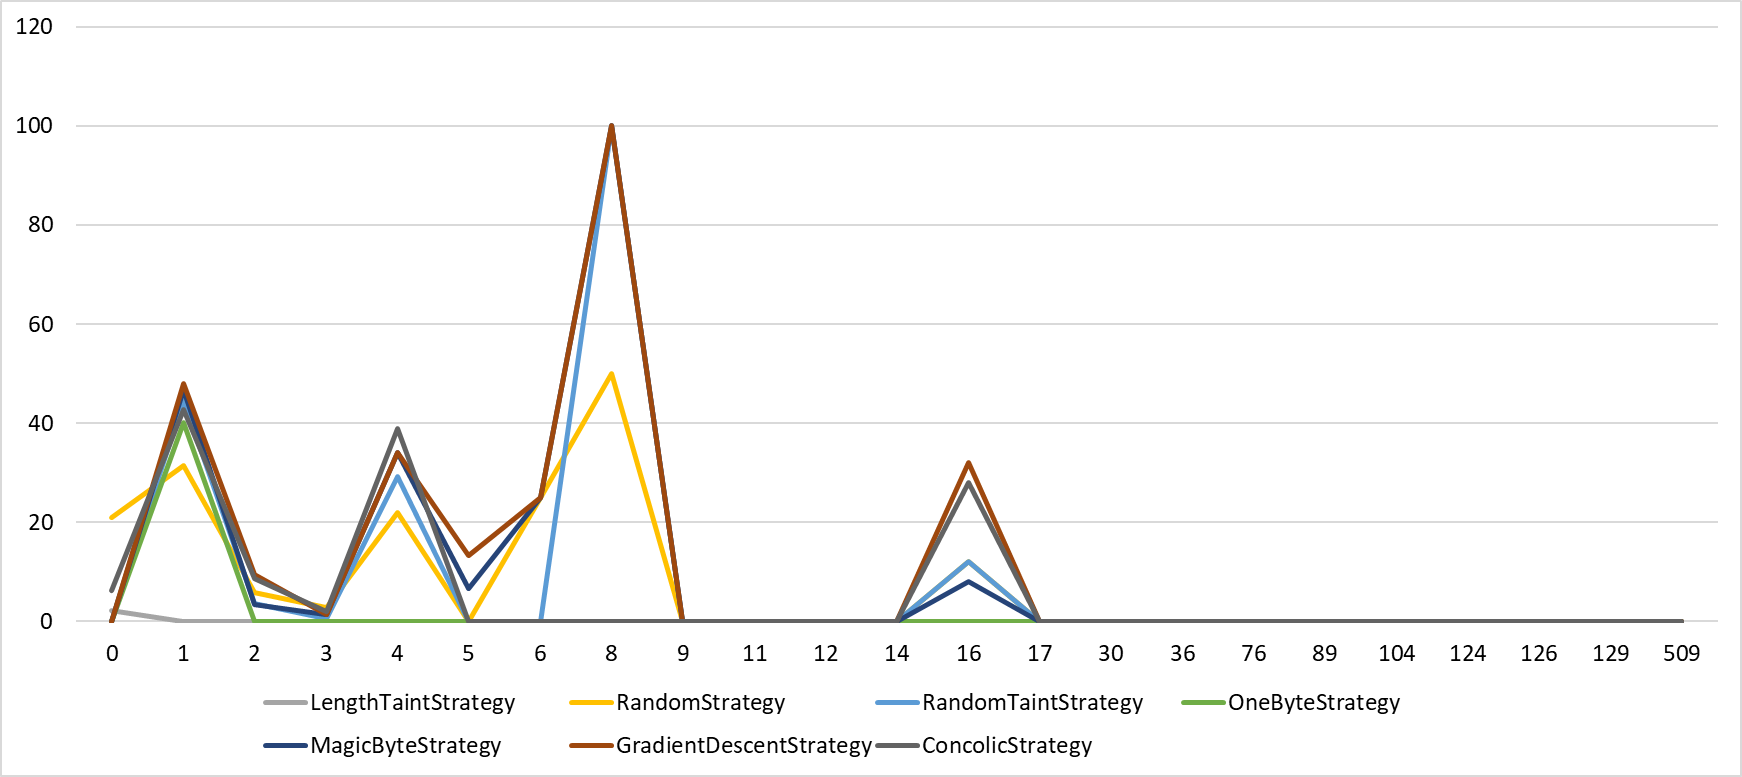
\includegraphics[width=.8\linewidth]{5_results/graphs/file-offsets.png}  
    \caption{Percentage of conditions flipped per number of offsets present from the input in the \texttt{file} binary.}
    \label{fig:fileOffsets}
\end{figure}

In the \texttt{file} program, we find that some condition exists, for which 509 offsets from the input were required to flip which can be seen in Figure \ref{fig:fileOffsets}. We see further peaks at some offsets, but no condition with more than 16 offsets were flipped.
\begin{figure}[H]
    \centering
    % include first image
    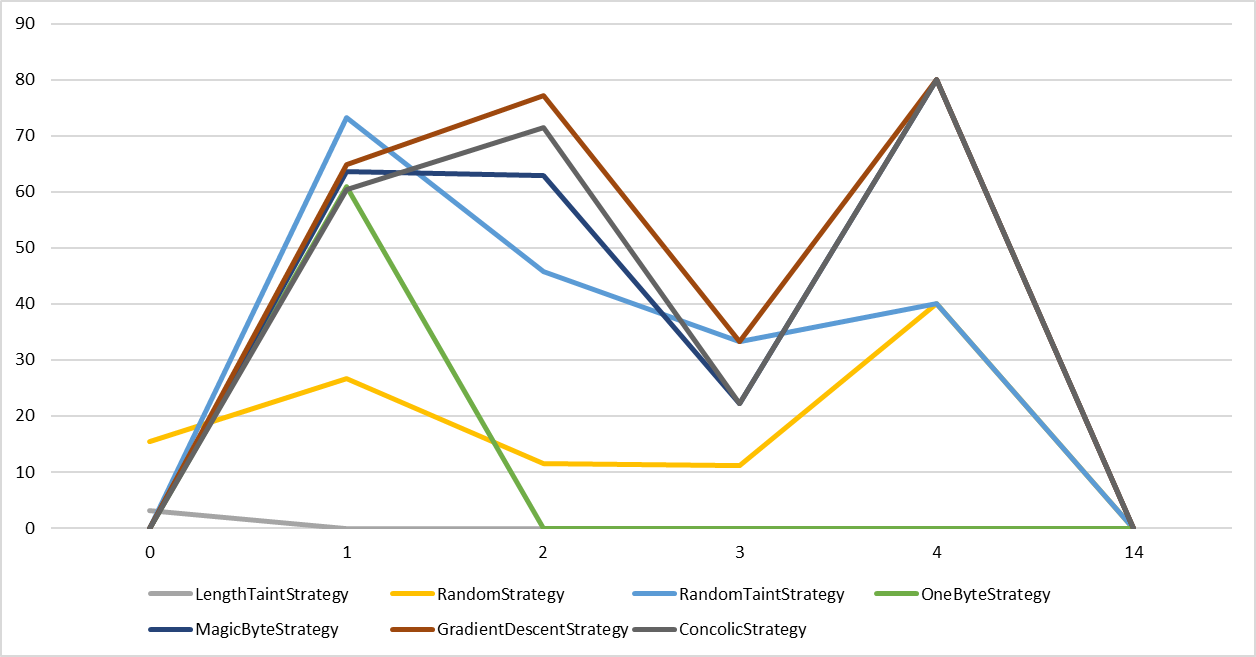
\includegraphics[width=.8\linewidth]{5_results/graphs/gif2png-offsets.png}  
    \caption{Percentage of conditions flipped per number of offsets present from the input in the \texttt{gif2png} binary.}
    \label{fig:gif2pngOffsets}
\end{figure}
Again we see that the RandomStrategy creates flips for conditions for which no offsets were found in Figure \ref{fig:gif2pngOffsets}. This further enhances the idea that some information is lost during the taint tracking. We see that the MagicByte strategy finds more flips than the GradientDescent strategy for only 1 offset, but less for the other offsets.
\begin{figure}[H]
    \centering
    % include first image
    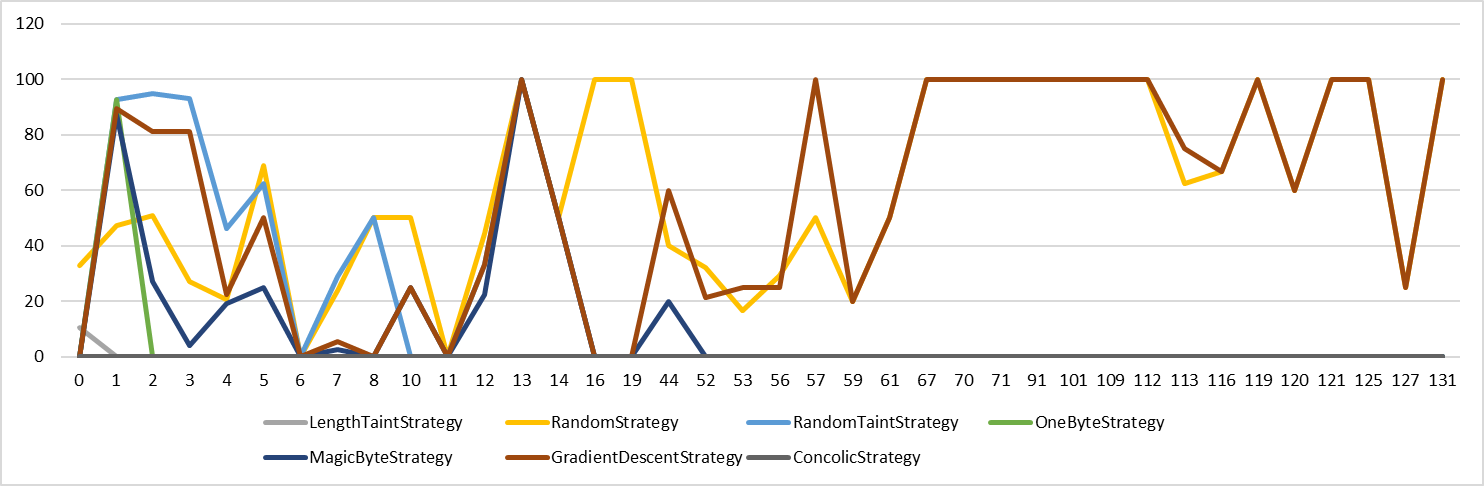
\includegraphics[width=.8\linewidth]{5_results/graphs/xmlwf-offsets.png}  
    \caption{Percentage of conditions flipped per number of offsets present from the input in the \texttt{xmlwf} binary.}
    \label{fig:xmlwfOffsets}
\end{figure}
We see in Figure \ref{fig:xmlwfOffsets} that even with a high number of offsets, the random strategy and GradientDescent strategy and RandomStrategy find flips for conditions with more than 100 offsets present in the input.
\begin{figure}[H]
    \centering
    % include first image
    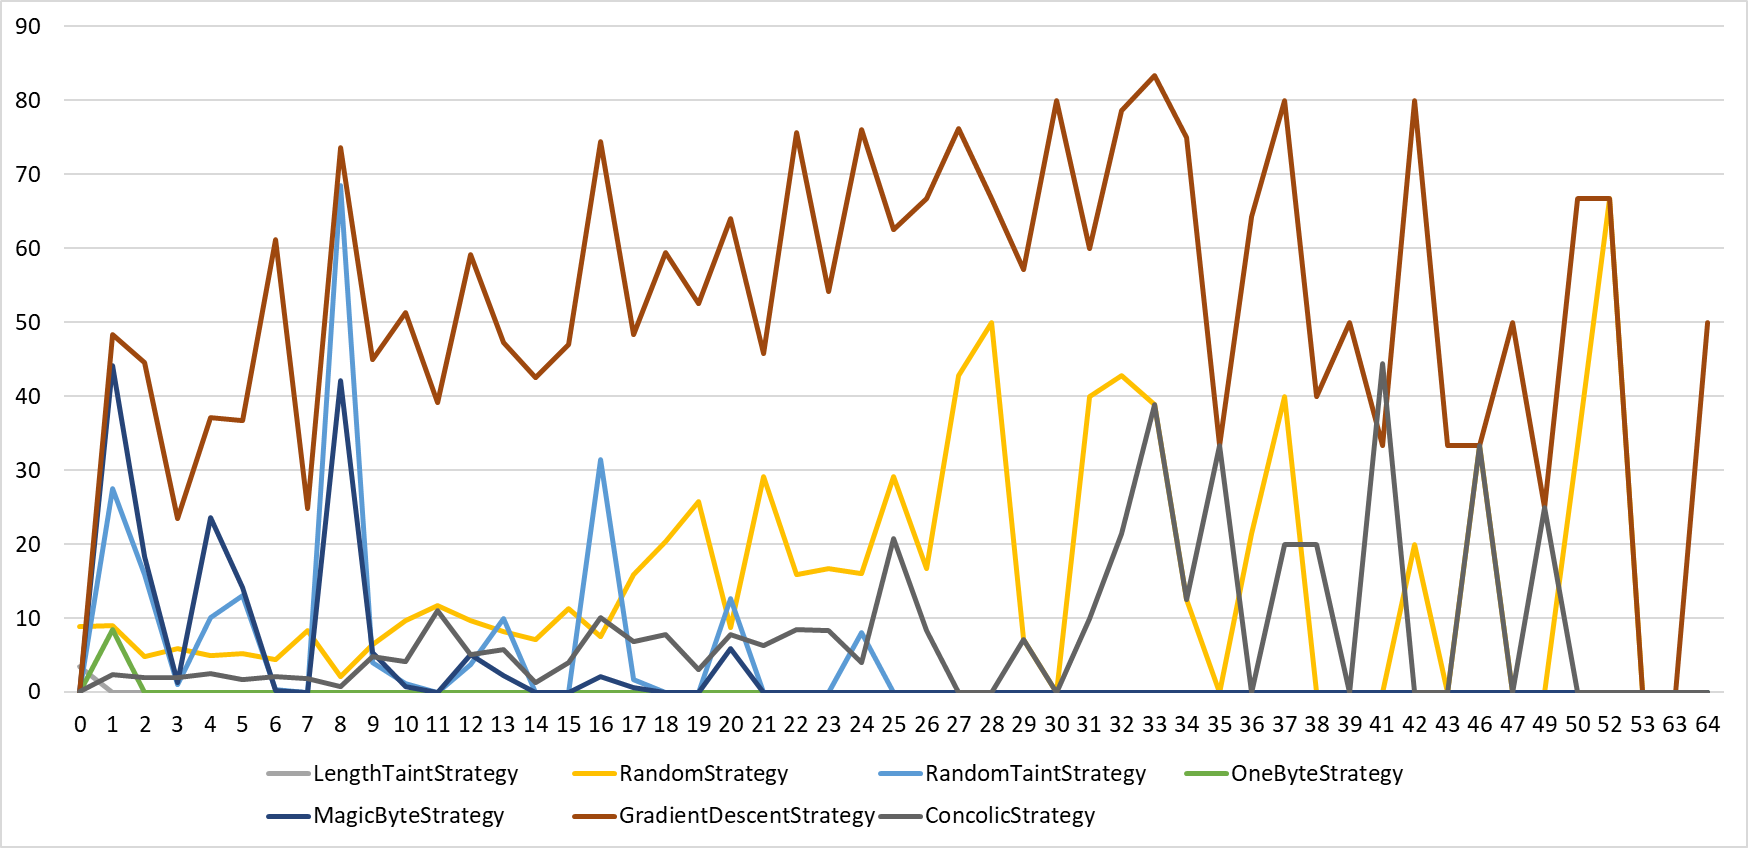
\includegraphics[width=.8\linewidth]{5_results/graphs/nm-offsets.png}  
    \caption{Percentage of conditions flipped per number of offsets present from the input in the \texttt{nm} binary.}
    \label{fig:nmOffsets}
\end{figure}
We see in Figure \ref{fig:nmOffsets} that the RandomTaintStrategy finds no flips for conditions with more than 25 offsets in the input, but the gradient descend and ConcolicStrategy do find flips for more flips. The RandomStrategy still finds flips which the RandomTaint strategy does not, which might indicate that we randomize too much in the RandomTaintStrategy.

From these graphs we get the idea that again the structure of the binary determines which strategy works better. This is because for the \texttt{xmlwf} and \texttt{nm} binary a lot of flips were found for conditions with a large number of offsets, but not for the \texttt{file} binary.




\subsection{Time}
In this section we will look at the time spend in a strategy.
Mostly because we want to know the effectiveness of the strategies. For this, we give the average of every strategy with the minimum and the maximum per binary. We expect the ConcolicStrategy to use a lot of time, but the other strategies way less.
The results are shown in Table \ref{appendix:timings} in seconds.
We notice that for the \texttt{file} binary, the ConcolicStrategy has ran for more than 10 seconds. After inspection, this could happen when a concolic run does not generate results, but the system call to terminate the process does not return immediately.
We indeed conclude that the ConcolicStrategy is several orders of magnitude slower than the other strategies for every binary. The MagicByte and OneByteStrategy only continue with the strategy if offsets are present, so the average gets influenced by the large number of executions where only a single check was performed.
This is also the case for the GradientDescentStrategy. Only for the runs of the \texttt{nm} binary, the Concolic execution is faster than expected. It is still unclear why this is the case. 
We further notice that the difference in speed between the Concolic and other strategies can be a factor 10 to 100 times faster on average. So symbolic execution should really be used as a last case resort if you want to preserve speed, which is also what \cite{stephens2016driller} and \cite{han2019synfuzz} use as approach to hybrid fuzzing.



% this file is called up by thesis.tex
% content in this file will be fed into the main document

\chapter{Evaluation}\label{chap:evaluation} % top level followed by section, subsection
In this chapter we will present the results found by our framework, and some challenges we encountered during the gathering of the results.

\section{Setup}
We ran the framework on Ubuntu 18.04 LTS inside a QEMU virtual environment with 62 CPU cores on an AMD ThreadRipper 2990WX processor with 64GB of RAM on which we also compiled the binaries and collected the traces.

We compiled every binary 5 times, twice with the modified Angora compiler, namely one for the fast instrumentation and one with the track instrumentation, once with the \texttt{SymCC} compiler, once with the Fuzz Checker compiler to create the Oracle and once with the static analysis pass.

We collected the traces by letting the fuzzer run for 8 hours on all 62 cores. Then we gave every strategy a maximum of 15 seconds of execution time per condition in a trace. We have chosen this limit because even the ConcolicStrategy could often finish within this time. For the ConcolicStrategy, we give it 13 seconds to calculate the possible executions and the last 2 seconds can be used to try the generated inputs. The execution time of the target binary is included in the execution time of a strategy, since the total time is the time one is interested in when trying to implement the most efficient strategy. The strategies which use randomness, like the RandomTaintStrategy, RandomStrategy and GradientDescentStrategy are executed 5 times, and then the average time to flip is computed for every condition. If any of the 5 runs managed to flip a condition, the condition is set to flipped. We took 5 runs to calculate the average, because of timing constraints.


\section{Results}
In this Section we will show per target binary the effectiveness of a strategy. First we will look at the performance of the strategy by looking at the percentage of flipped conditions and by ranking the strategies by the time it took to flip conditions. We will also inspect the substrategies for the strategies which used these. Then we will inspect the results of the microbenchmarks to see when a strategy fails to flip a branch. After this, we will inspect the collected metrics of the branches and try to find any relation between the performance and these metrics.

\subsection{Flipped conditions}
Since coverage in increased then conditions are flipped, one of the most important measures of performance is the number of flipped conditions. In Figure \ref{fig:flipped-conditions} we show the percentage of flipped conditions out of the total tried conditions per strategy and per program. Since all strategies except the RandomStrategy only work on conditions with taint information, we also added a separate column of the conditions flipped by the RandomStrategy which have taint information available to better compare the results.

\begin{figure}[H]
    \centering
    % include first image
    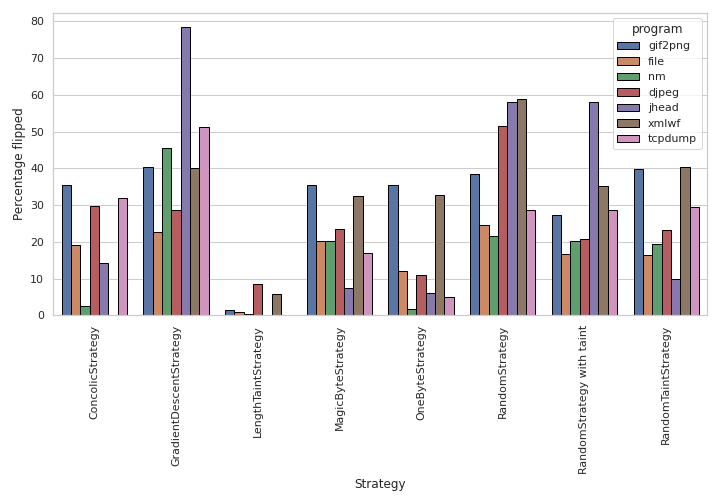
\includegraphics[width=0.8\textwidth]{5_results/graphs_new/percentage_flipped_total.png}  
    \caption{Percentage of all flipped conditions per program}
    \label{fig:flipped-conditions}
\end{figure}

We see that there is quite some difference between the performance of a strategy per program. It appears that the GradientDescentStrategy outperforms the RandomStrategy with taint in most cases, while the LengthTaintStrategy underperforms most other strategies. We also notice that the number of conditions which are flipped by the RandomStrategy with and without taint differ quite a bit per program. Between the \texttt{xmlwf} binary and the \texttt{djpeg} binary, there is a large decrease in the percentage of flipped conditions when only conditions with taint are considered. This looks like the RandomStrategy sometimes flips a lot of conditions which do not have taint information.
However, since we might be working with biased data, we want to look further than the GradientDescentStrategy. So the next best strategies when considering percentage of flipped conditions are the RandomStrategy and the RandomTaintStrategy.

We also want to compare the individual conditions. We inspect if there is overlap between the flipped conditions by comparing every strategy with every other strategy. We first take the set of all flipped conditions by one strategy as superset. Then we take all flipped conditions from another strategy as subset and compare how much of the subset is present in the superset. The results are visible in Figure \ref{fig:overlap-strategies}.

\begin{figure}[H]
    \centering
    % include first image
    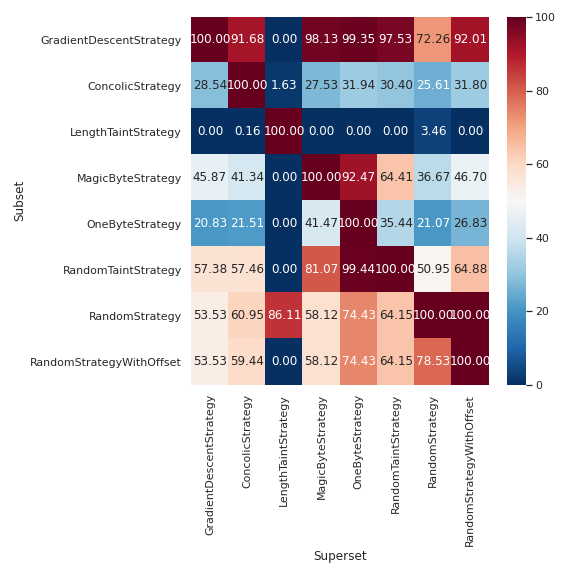
\includegraphics[width=0.75\textwidth]{5_results/graphs_new/overlap_strategies.png}  
    \caption{Percentage of overlap between the super and subset.}
    \label{fig:overlap-strategies}
\end{figure}

Here we notice that for nearly every strategy more than 90\% the flipped conditions are also found by the GradientDescentStrategy. The exception is the LengthTaintStrategy and when only considering the RandomStrategy when also looking at conditions with no taint. From this we expect that the GradientDescentStrategy is a good strategy when trying to flip conditions where taint information is available, and that the RandomStrategy is useful when trying condition when no taint information is available. The LengthTaintStrategy should also be applied to flip the conditions missed by the GradientDescentStrategy.

To conclude that these results also translate to a significant difference, we follow the statistical test used in \cite{metzman2020fuzzbench, demvsar2006statistical}. We need a non-parametric test, so we do not have to make assumptions on the shape of the data, hence we take the Friedman test. 
We have as null-hypothesis that there is no difference in the average number of flipped conditions between all strategies. We obtain a p-value of $3.62 \cdot 10^{-5}$, hence we reject our null-hypothesis with $\alpha = 0.05$, as we conclude that there is a significant difference between the strategies. Now we can perform a post-hoc Nemenyi test to see which individual strategies are significantly different from one another, again with  $\alpha = 0.05$.
The results are visible in Figure \ref{fig:cd-strategies}.

\begin{figure}[H]
    \centering
    % include first image
    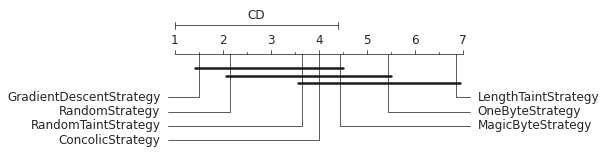
\includegraphics[width=0.8\textwidth]{5_results/graphs_new/cd_strategies.png}  
    \caption{Critical distance between average rank of the strategies.}
    \label{fig:cd-strategies}
\end{figure}

The strategies connected via a bold line are not statistically different from one another. The numbers shown are the average rank of the performance of the strategies, so closer to 1 means `first place' of a total of 7 positions.

Predictably, when we split the data between the OneByteStrategy and LengthTaintStrategy on one side and all other strategies on the other side, there is a significant difference between these groups. These strategies are rarely used, so they have the least amount of total flips. 
Interestingly enough, there is also a significant difference when we group the GradientDescentStrategy and RandomStrategy on the one side and the other strategies on the other side, which seems to confirm our results from Figure \ref{fig:overlap-strategies}.

We repeated this experiment but now replacing the flipped conditions found by the RandomStrategy by the conditions which were flipped which had taint information available. We obtained a p-value of $1.19 \cdot 10^{-4}$ by the Friedman test. The results are visible in Figure \ref{fig:cd-strategies-with-taint}.
\begin{figure}[H]
    \centering
    % include first image
    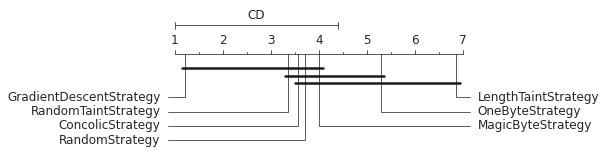
\includegraphics[width=0.8\textwidth]{5_results/graphs_new/cd_strategies_with_offset.png}  
    \caption{Critical distance between average rank of the strategies only considering tainted conditions.}
    \label{fig:cd-strategies-with-taint}
\end{figure}
We get somewhat similar results, but now it is clear that the GradientDescentStrategy is statistically different from all other strategies except the RandomTaintStrategy when considering only conditions which have taint information available. When we keep in mind that the collected traces might have a bias towards the GradientDescentStrategy, we also see that the RandomTaintStrategy is statistically different from the other strategies excluding the GradientDescentStrategy.

\subsection{Time to flip}
The percentage of flipped conditions is not the only measure we have to compare the performance. We also measured the time a strategy spend mutating an input until a flip was found in a given condition. To compare the timing of the strategies, we rank the time a strategy took before a given condition was flipped for all conditions which have been flipped at least once. If a condition was never flipped by a strategy, we assign the maximum rank.
The mean ranks can be found in Figure \ref{fig:rank} the black lines are the confidence interval of 95\% of the data.
\begin{figure}[H]
    \centering
    % include first image
    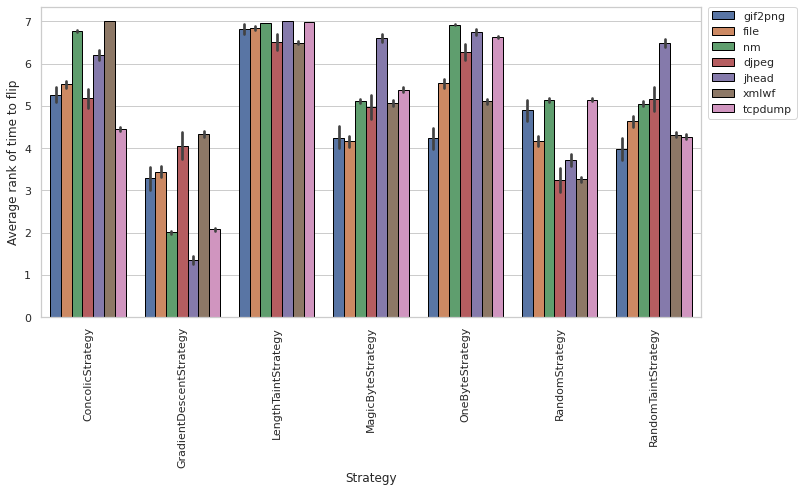
\includegraphics[width=1\textwidth]{5_results/graphs_new/ranks_with_time.png}  
    \caption{Average rank of the time to flip a condition per program}
    \label{fig:rank}
\end{figure}
Again the GradientDescentStrategy has the lowest rank and seems the fastest. 
We should watch out for data bias here, since there were a lot of flips found using the GradientDescentStrategy, it has more conditions where it was the only strategy which flipped the conditions, and this might skew the results.

We want to check if this result is also significant.
We have as null-hypothesis that there is no difference in the time to flip a condition between all strategies. If we perform a Friedmann test, we obtain a p-value of $3.34 \cdot 10^{-5}$, hence we reject our null-hypothesis with $\alpha = 0.05$, as we conclude that there is a significant difference between the strategies. Now we can perform a post-hoc Nemenyi test to see which individual strategies are significantly different from one another, again with  $\alpha = 0.05$. The results are visible in Figure \ref{fig:cd-strategies-with-rank}.
\begin{figure}[H]
    \centering
    % include first image
    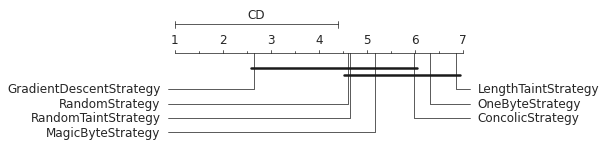
\includegraphics[width=0.8\textwidth]{5_results/graphs_new/CD_rank_timing.png}  
    \caption{Critical distance between average rank of the strategies only considering flipped conditions.}
    \label{fig:cd-strategies-with-rank}
\end{figure}
So here we see that there is a significant difference between the time of the GradientDescentStrategy against all other strategies.

\subsection{Substrategies}
We also looked at the used substrategies and their effectiveness.
We applied the strategies in the order as shown in Figure \ref{fig:substrategies}. If a condition was flipped by one substrategy, the next substrategy is not tried anymore. The results are shown in Figure \ref{fig:substrategies}.
We only look at flipped conditions, and using the MagicByteStrategy we see that the fill\_in substrategy is quite effective, just like the arithmatic substrategy which adds 1 byte. The zero extensions also seem to flips some extra conditions, but the encoding transformations do not seem to find a lot of extra flips.

The GradientDescendStrategy finds the same flips as the MagicByteStrategy due to the use of the substrategies, hence this strategy always outperform the other, and as additional bonus, it then picks a random starting point and restarts the GradientDescendStrategy from this input, where it repicks a random input when it is stuck in a local optimum. Hence this combines a part of the RandomTaintStrategy, and it shows that of all the flips found by this strategy at least 25\% and up to 70\% of all flips for the \texttt{tcpdump} binary are found using the random substrategy.
\begin{figure}[H]
    \centering
    % include first image
    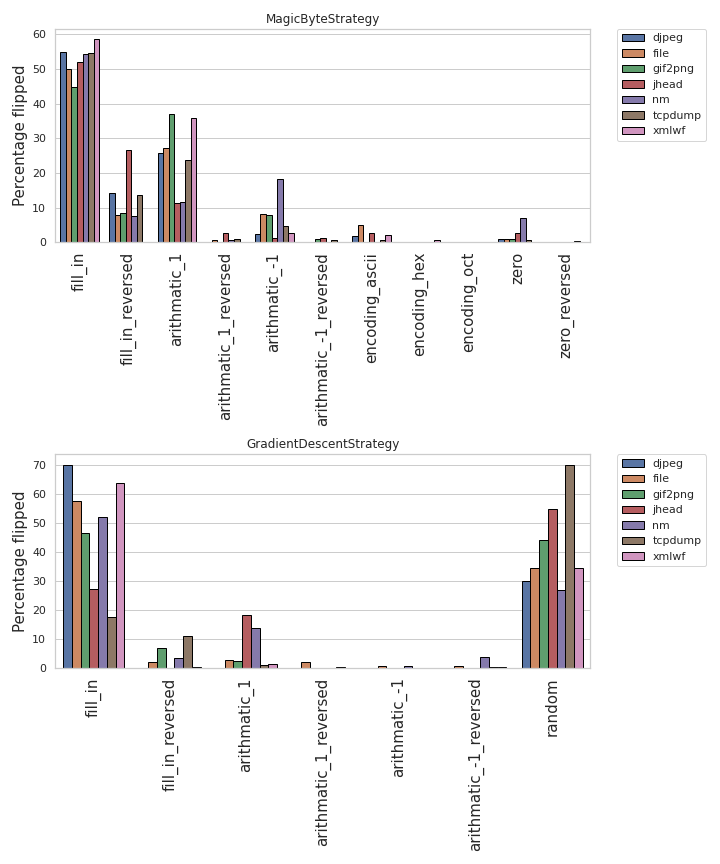
\includegraphics[width=0.8\textwidth]{5_results/graphs_new/substrategy_overview.png}  
    \caption{Distribution of flipped conditions by substrategy.}
    \label{fig:substrategies}
\end{figure}

\subsection{Microbenchmarks}
We also looked at the reasons why a strategy did not flip a condition. Here we see some expected results and some unexpected results.
The RandomStrategy is always tried, hence it can only be one of two reasons why it did not flip a condition, it either never reached the condition or it reached the conditions but the condition was not flipped. Only 15\% of the time did it never reach the condition, while in 85\% of the times it did reach the condition. The OneByteStrategy and LengthTaintStrategy are often never tried, as expected since these trigger only under special circumstances.
When we compare this with the RandomTaintStrategy, we see that it skips about 22\% of all cases, because there is no taint information available and of the tried inputs, over 50\% never reaches the condition it is trying to fuzz. The MagicByteStrategy reaches even less, over 60\% of the conditions are not reached.
Another curious case is the ConcolicStrategy, which apparently in about 58\% of the cases cannot generate any input for the condition.

\begin{figure}[H]
    \centering
    % include first image
    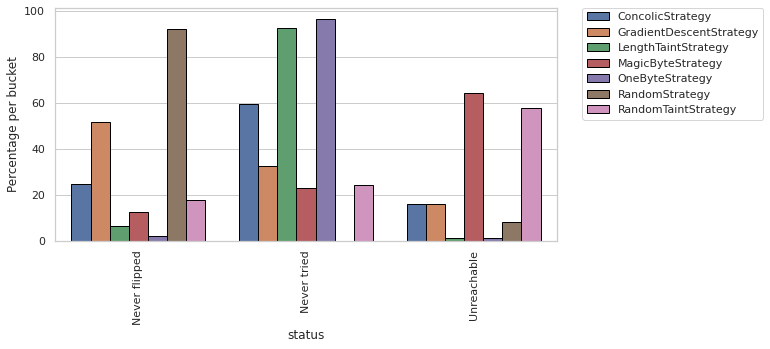
\includegraphics[width=0.8\textwidth]{5_results/graphs_new/benchmarks.png}  
    \caption{Distribution of not flipped conditions by micro-benchmark.}
    \label{fig:benchmarks}
\end{figure}

\subsection{Relation to metrics}
With some of the metrics we choose, we were not sure if this metric was helpful in providing any kind of information about the conditions. So the first thing we test is if we choose the right metrics. We want to know if there is a significant difference between the distribution of the metrics of the flipped conditions versus the distribution of the metrics of the non flipped conditions. If the relation between the metric and the flipped condition is independent, the distribution of the metric should be equal for flipped and not flipped conditions. However, if the metric is related to the result of the tried condition, the distribution should differ.
We perform a non-parametric Mann-Whitney U test \cite{metzman2020fuzzbench}, where the null hypothesis is that there is no difference in the distribution between the flipped and not flipped conditions. We want to look at the different distributions when we split the data per metric, but also per program. So we perform the test for every combination between metric and program. The results are visible in Figure \ref{fig:mann-whitney-program-metrics}.

\begin{figure}[H]
    \centering
    % include first image
    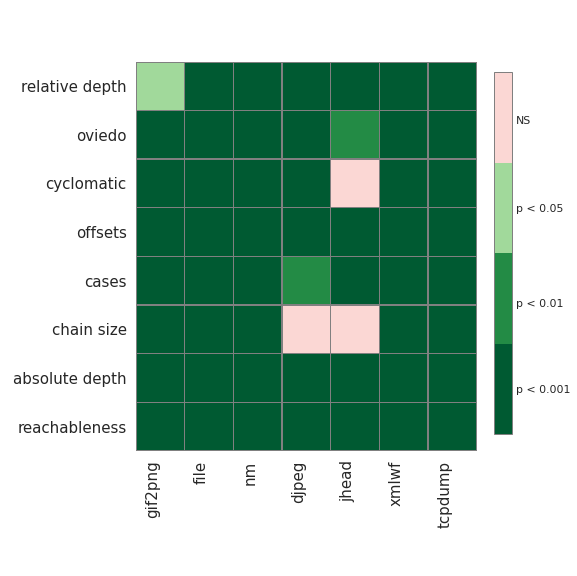
\includegraphics[width=0.8\textwidth]{5_results/graphs_new/mann_whitney_u_programs.png}  
    \caption{Results of the Mann-Whitney U test between programs and metrics}
    \label{fig:mann-whitney-program-metrics}
\end{figure}
Here we see that for any program, there is a significant difference in the distribution between the flipped and not flipped conditions for nearly all programs. Only the \texttt{djpeg} and \texttt{jhead} programs do not have a significant difference everywhere.

We are also interested in the difference between the strategies and the metrics, since this could be used to say which metric can predict the behaviour of a strategy. We again performed the test between every metric and strategy as shown in Figure \ref{fig:mann-whitney-strategy-metrics}.
\begin{figure}[H]
    \centering
    % include first image
    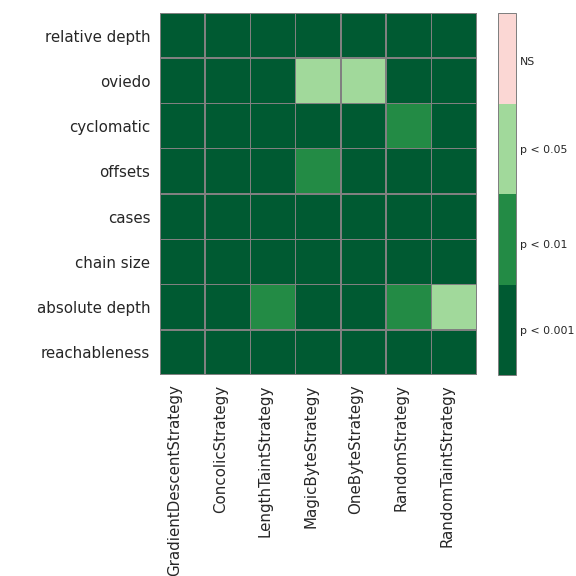
\includegraphics[width=0.8\textwidth]{5_results/graphs_new/mann_whitney_u_strategy.png}  
    \caption{Results of the Mann-Whitney U test between strategies and metrics}
    \label{fig:mann-whitney-strategy-metrics}
\end{figure}
We find that all metrics have a significant difference in the distribution between the flipped and not flipped conditions. 
This means that we should be able to differentiate between conditions which will be flipped and not be flipped based on our chosen metrics. In the next Section we will build a classifier which does this.

We further inspect the relation of the metrics with the strategies, now by focusing on our flipped conditions and the strategies which flipped the conditions.
We want to know when a metric results in the highest number of flips. For example, we expect that the number of flipped conditions decreases when the reachableness increases. However, we are also interested in the relation with the total time spend on a condition and the relative depth of the program when the condition was flipped.
We have constructed a kernel density estimation of where in the program, by looking at the relative depth, conditions where flipped in Figure \ref{fig:kde-relative}.

\begin{figure}[p]
    \centering
    % include first image
    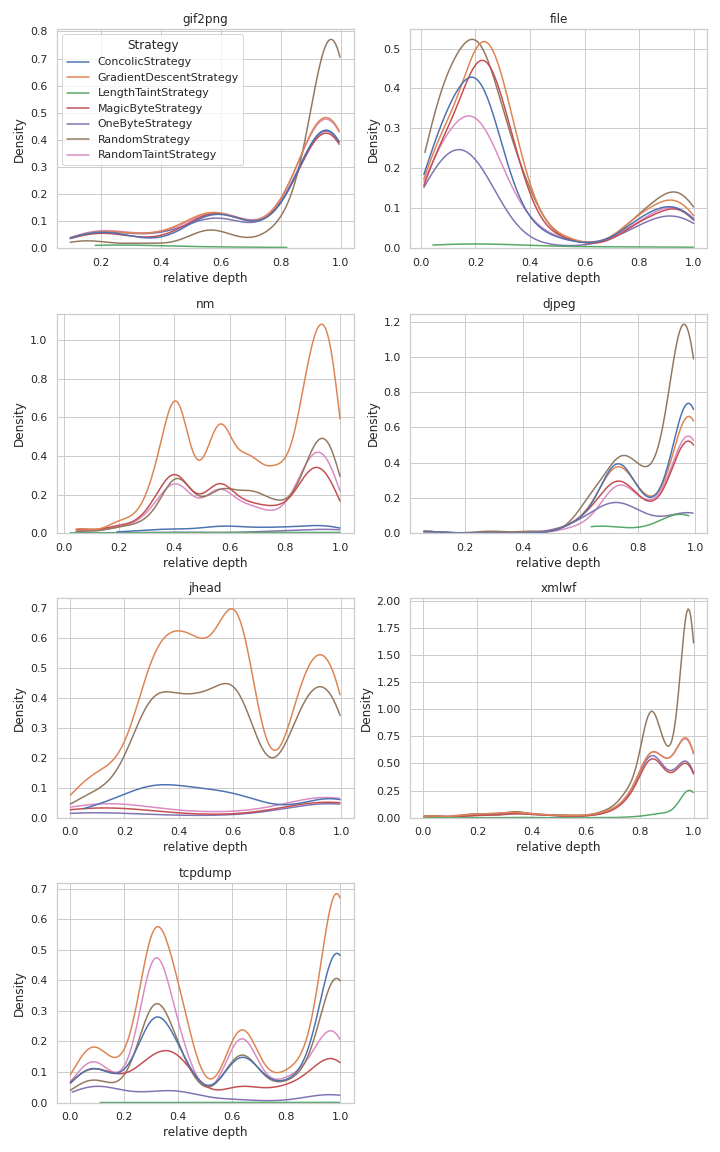
\includegraphics[width=0.9\textwidth]{5_results/graphs_new/kde_relative.png}  
    \caption{Kernel density estimation plots of the relative depth per program}
    \label{fig:kde-relative}
\end{figure}
We see that the depth where the conditions are flipped differs between programs. Some programs have more flipped conditions at the end, like \texttt{gif2png} and \texttt{xmlwf}, while other like \texttt{jhead} seem to find more flipped conditions in the middle. It looks like there are some `hotspots' in the programs where more conditions are flipped than in other locations. 

Another notable result, is that most strategies are grouped together, when one strategy finds flipped conditions, others also find flipped conditions at the same locations.
%In the \texttt{jhead} binary, it is visible that the GradientDescentStrategy outperforms the other strategies, but also the RandomStrategy outperforms the other strategies here.

The reachableness metric is shown in Figure \ref{fig:kde-reachableness} with a cutoff at 200, since there were some extreme values. Here the strategies also seem to follow one another closely for some programs, for example in the \texttt{gif2png} binary, or with distinct peaks in the \texttt{jhead} binary. The plots confirm our suspicion, most flipped conditions occur when the reachability is low, hence there are not many bytes compared in the conditions or before the condition. This means this is likely a good metric to include in our models.

%We have shown that for some variables, the graphs look cautiously optimistic when looking for a relation.

\begin{figure}[p]
    \centering
    % include first image
    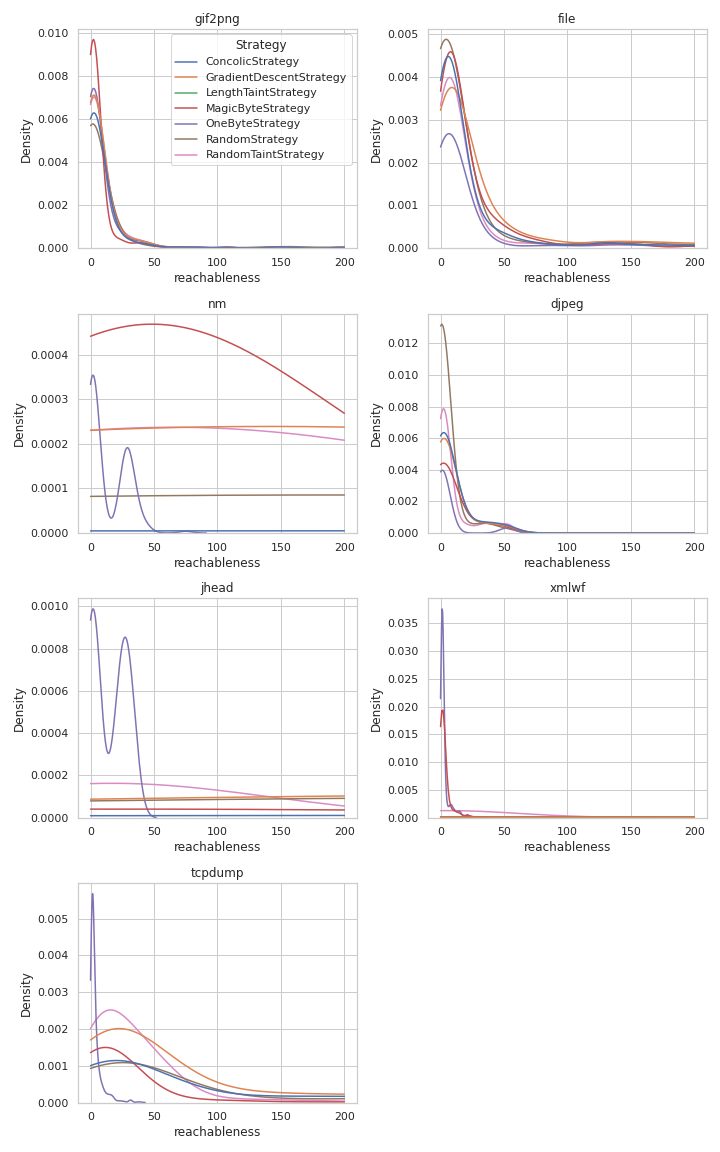
\includegraphics[width=\textwidth,height=\textheight,keepaspectratio]{5_results/graphs_new/kde_reachableness.png}  
    \caption{Kernel density estimation plots of reachableness per program}
    \label{fig:kde-reachableness}
\end{figure}

Another important measure of performance is the time a strategy has spend on a condition. We again look at a kernel density estimation plot with the time on a logarithmic scale. We plotted the time on a logarithmic scale, since a lot of flipped conditions take a fraction of a second, while others take over 10 seconds.
We see that a lot of strategies manage to finish within a second, but some strategies take longer, like the RandomStrategy which also has a peak a little before 15 seconds. This is possibly due to the multiple runs of this strategy, where if one run manages to flip a condition, we still take the average time. If other runs did not manage to find a flip, those runs timeout at 15 seconds. Hence the average lays close to 15. It is notable that other strategies often find the flip within the first second, even the more advanced strategies like the GradientDescentStrategy.
Since there is so much data in the first second, where the differences are small, we expect that predicting the fastest strategy with machine learning models can be a problem.


\begin{figure}[H]
    \centering
    % include first image
    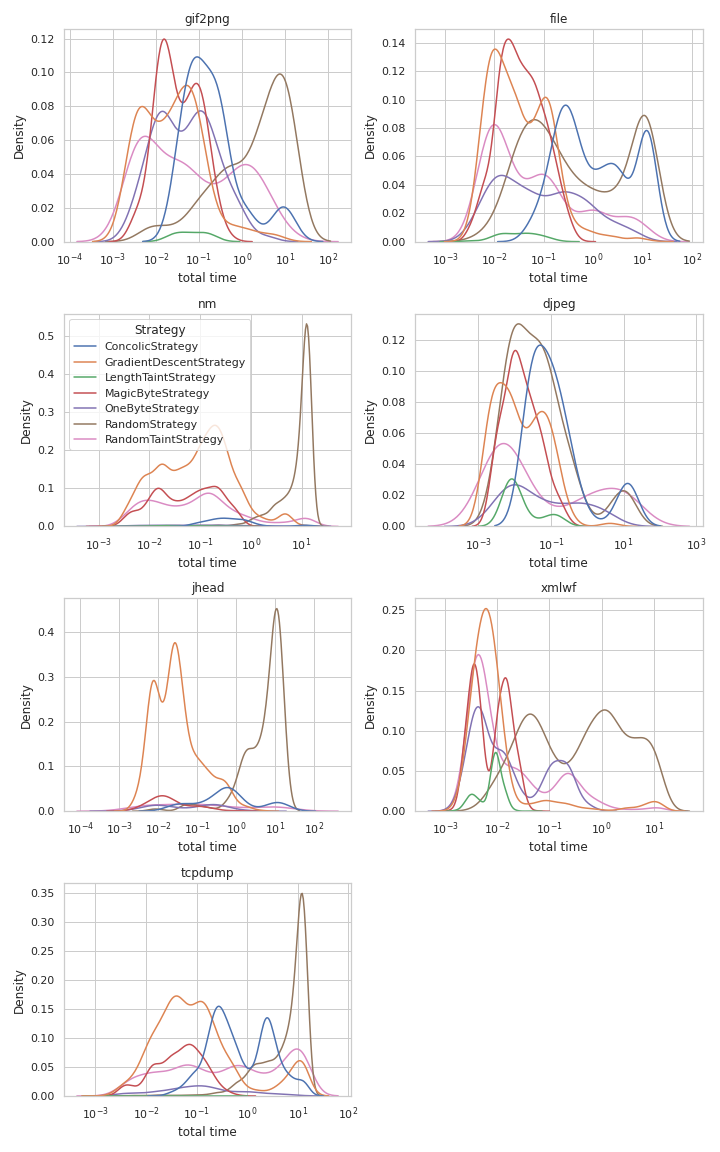
\includegraphics[width=\textwidth,height=\textheight,keepaspectratio]{5_results/graphs_new/kde_flipped_timing.png}  
    \caption{Kernel density estimation plots of total time per program}
    \label{fig:kde-timing}
\end{figure}

From the timing plots, we see interesting behaviour of the ConcolicStrategy, which appears to be done within the time limit. We found that the ConcolicStrategy needs on average $1.85$ seconds to flip a branch when offsets are available, while it takes on average $10.59$ seconds when no offset information is available. This shows that a combination of dynamic taint analysis and symbolic execution can increase the average speed of a symbolic strategy nearly tenfold. This is shown in Table \ref{tab:concolic-info}.

\begin{table}[H]
\centering
\begin{tabular}{l|rr}
\toprule
Strategy &  Offsets available &  No offsets available \\
\midrule
count &            6287 &                118 \\
mean  &               1.85 &                 10.59 \\
std   &               3.00 &                  5.06 \\
min   &               0.02 &                  0.04 \\
25\%   &               0.23 &                 11.81 \\
50\%   &               0.48 &                 13.09 \\
75\%   &               2.31 &                 13.23 \\
max   &              14.98 &                 14.98 \\
\bottomrule
\end{tabular}

\caption{Timing information of the ConcolicStrategy where a condition was flipped}\label{tab:concolic-info}
\end{table}

Other plots are less interesting and can be found in Figure \ref{fig:kde-flipped-conditions}. An unexpected result is that most strategies seem to find flips for the same metrics, except the LengthStrategy.

%After this analysis, we can create models with the goal of predicting properties of a condition with only the metrics as input.

\section{Creating models}
In the previous Section, we found that some strategies seem to outperform others when looking at the overall performance. However, we also found a significant difference between the distribution of the flipped and not flipped conditions when comparing different strategies and metrics. So we create models as explained in Section \ref{sec:overview}. In the field of machine learning, the collected metrics are called features. To be consistent in this naming convention we will refer to the individual metrics in this Section by calling them features.

\subsection{Feature selection}
The first step in our model creation is the selection of the right features.
Not all features are important when creating the models and some features can be correlated with one another. We filter the features which have a high correlation and analyse which of the remaining features are more important than others.

To calculate the correlation, we use Spearman's rank correlation coefficient \cite{lehman2005jmp} as shown in Figure \ref{fig:correlation}. Here we calculate this coefficient for every program separately for every combination of features.
\begin{figure}[p]
    \centering
    % include first image
    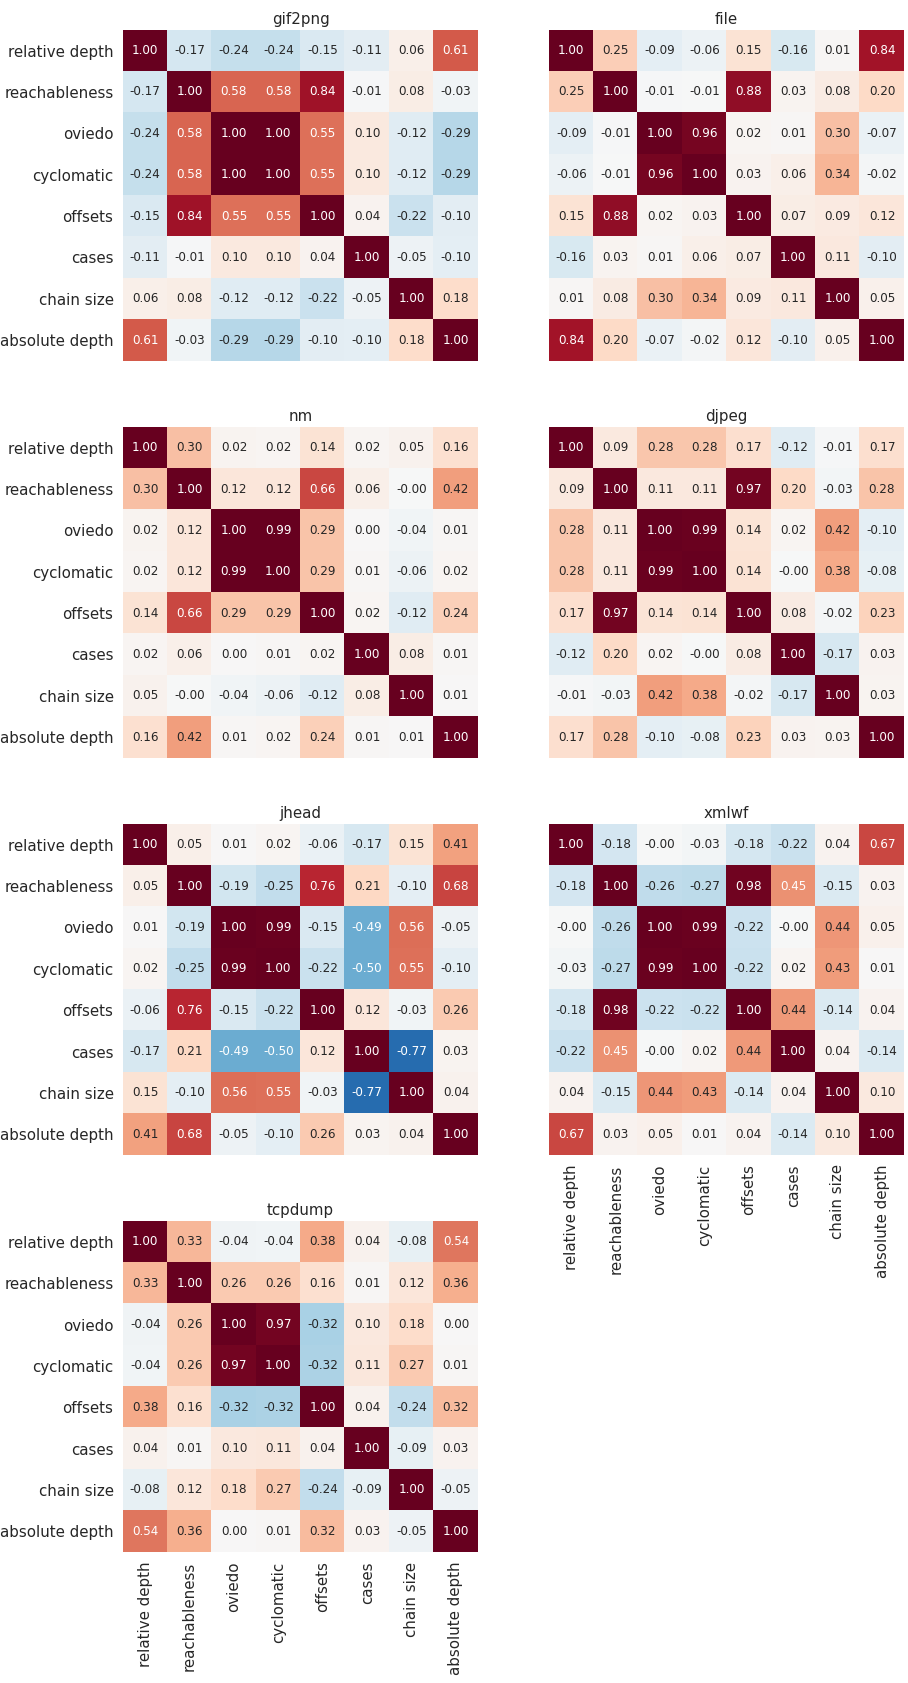
\includegraphics[height=\textheight]{5_results/graphs_new/correlation_benchmarks.png}  
    \caption{Heatmap of correlation coefficients between all features per program}
    \label{fig:correlation}
\end{figure}
We see that the Oviedo and the cyclomatic complexity are highly correlated, nearly one-on-one. We also notice that the reachableness and offsets are highly correlated, since the reachableness metric is more specific case of the offsets metric, however not in all cases.

Our next step is calculating the mutual information for every feature and the flipped conditions. When this value equals 0, it means that the variables are independent, so they cannot be related to one another, higher values indicate that it can be used to estimate if a condition can be flipped. The results are displayed in Figure \ref{fig:feature-importance}.

\begin{figure}[H]
    \centering
    % include first image
    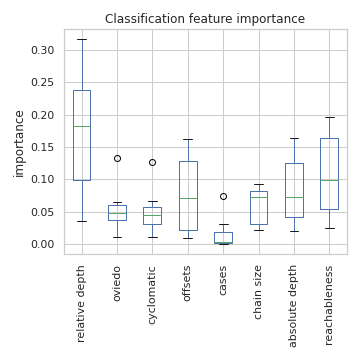
\includegraphics[width=0.5\textwidth]{5_results/graphs_new/feature_selection.png}  
    \caption{Mutual information per feature for the flipped conditions}
    \label{fig:feature-importance}
\end{figure}

We see that the relative depth has the highest average importance, and the cases feature often is of very low importance. The offsets and reachablesness are also important features, and Oviedo complexity and the chain size are not the highest, but we still include them. This gives us the selected features: relative depth, Oviedo complexity,  offsets, chain size and reachableness. We disregard the absolute depth metric, because we already have the relative depth, and the absolute depth has a lower importance than the relative depth.

For the model which predicts the time, we have to look at the mutual information between the selected features and the total time while considering only the flipped conditions. The results are given in Figure \ref{fig:feature-importance-regressor}.

\begin{figure}[ht]
    \centering
    % include first image
    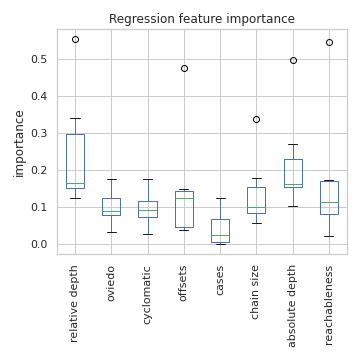
\includegraphics[width=0.5\textwidth]{5_results/graphs_new/feature_selection_regression.png}  
    \caption{Mutual information per feature for the total time}
    \label{fig:feature-importance-regressor}
\end{figure}

We notice that the results are pretty similar, except that the absolute depth feature is more important than before, however, the relative depth has a slightly higher average, hence our selection of features does not change.

\subsection{Predicting flipped conditions}
To create a model which classifies a condition as flippable or not flippable, we train a number of machine learning models and assess their performance using the metrics described in Section \ref{sec:MLmodels}. We also try to find the best parameters by using 5-fold cross validation. To perform cross validation, the data is randomly split in a test set of 40\% and a training set of 60\% of the original data.
In Table \ref{tab:classifiers-overview} we give an overview of the tested models and the search space for their hyperparameters.
To see if it actually performed better, we also compared it using a DummyClassifier for every program. A DummyClassifier just returns the most frequent label from the training data, no mater what input is given.

In Table \ref{tab:classifiers-result} we show the best scores per model including the comparison with the DummyClassifier. We quickly notice that the DecisionTreeClassifier (DT) is in all cases the best model, except for the \texttt{gif2png} and \texttt{jhead} binary and that the DummyClassifier is outperformed everywhere.
\begin{table}[H]
\centering
\begin{tabular}{lllll}
\toprule
{} &        Best precision &           Best recall &         Best f1-score &         Best accuracy \\
\midrule
gif2png &  0.700 (DT) &       0.685 (Gausian) &       0.687 (Gausian) &       0.685 (Gausian) \\
file    &  0.902 (DT) &  0.903 (DT) &  0.902 (DT) &  0.903 (DT) \\
nm      &  0.840 (DT) &  0.840 (DT) &  0.840 (DT) &  0.840 (DT) \\
djpeg   &  0.860 (DT) &  0.855 (DT) &  0.857 (DT) &  0.855 (DT) \\
jhead   &           0.843 (SVC) &           0.843 (SVC) &           0.843 (SVC) &           0.843 (SVC) \\
xmlwf   &  0.808 (DT) &  0.807 (DT) &  0.807 (DT) &  0.807 (DT) \\
tcpdump &  0.836 (DT) &  0.836 (DT) &  0.836 (DT) &  0.836 (DT) \\
\bottomrule
\end{tabular}

\caption{Models which scored the highest per scoring metric.}\label{tab:classifiers-result}
\end{table}
We achieve relatively good scores of slightly above 80\% accuracy and precision for most programs, except the \texttt{gif2png} binary. 
%Since we use a DecisionTreeClassifier, we can actually look at the decision tree and how the classifier is constructed as shown in Figure \ref{fig:decision-tree-gif2png}.
\begin{comment}
\todo{does this contribute to the paper?}
\begin{figure}[h]
    \centering
    % include first image
    \includegraphics[width=\textwidth,height=\textheight,keepaspectratio]{5_results/graphs_new/decision_tree.png}  
    \caption{Part of the decision tree of the \texttt{gif2png} binary.}
    \label{fig:decision-tree-gif2png}
\end{figure}
\end{comment}

We also recreated the models but now we used Principal Component Analysis (PCA) in order to reduce the number of features by transforming the data to a space where every column is orthogonal to the previous columns when interpreting the columns like vectors. Using this technique, we could explain 95\% of the variance variance with only 3 columns in our transformed dataset. However, the created classifiers performed overall, worse than the previous created classifiers. The results are shown in Table \ref{tab:classifiers-result-pca}.

\begin{table}[H]
\centering
\begin{tabular}{lllll}
\toprule
{} &        Best precision &           Best recall &         Best f1-score &         Best accuracy \\
\midrule
gif2png &           0.702 (SVC) &           0.705 (SVC) &           0.697 (SVC) &           0.705 (SVC) \\
file    &  0.832 (DT) &  0.831 (DT) &  0.831 (DT) &  0.831 (DT) \\
nm      &  0.688 (DT) &  0.688 (DT) &  0.688 (DT) &  0.688 (DT) \\
djpeg   &  0.806 (DT) &  0.801 (DT) &  0.803 (DT) &  0.801 (DT) \\
jhead   &       0.840 (Gausian) &       0.850 (Gausian) &  0.833 (DT) &       0.850 (Gausian) \\
xmlwf   &  0.757 (DT) &  0.751 (DT) &  0.753 (DT) &  0.751 (DT) \\
tcpdump &  0.764 (DT) &  0.765 (DT) &  0.764 (DT) &  0.765 (DT) \\
\bottomrule
\end{tabular}

\caption{Models which scored the highest per scoring metric after PCA.}\label{tab:classifiers-result-pca}
\end{table}
We note however, that these models were trained after the fuzzing runs were already performed. When we compare the constructed models of the programs between one another, the accuracy reaches 0.5, where it becomes no more powerful than a coin toss. Hence, if a fuzzer would use this approach, it would need to train the model during the fuzzing run for a specific program.

\subsection{Predicting time spend}
The next step is creating a model which tells us which strategy we should use when we find a flippable condition. We should pick a strategy which flips the condition the fastest. We can do this in one of two ways. We either create another classifier which predicts for a condition the fastest strategy, or we create a regression model to predict the time spend on a condition by a strategy and then select the strategy which is predicted to be the fastest. We should only select conditions where a flip occurs.

When using the classifier models as we did previously, we run into the problem that some strategies, or labels, only occur very infrequent in the results, which results in poor results when using 5-fold cross validation. When we compared the created classifiers with a DummyClassifier, this outperformed the created models for every program for every scoring metric. Hence we choose to create a regression model.

We again try a number of different regression models and estimate the best parameters using 5-fold cross validation. The tested models and the search space for the hyperparameters can be found in Table \ref{tab:regressor-overview}. The scores of the median average error seem to be rather low, they are all well under 1 second, which looks promising.
To see if the results make sense, we compare them to a DummyRegressor. This model just returns the median total time for every strategy.
When looking at the DummyRegressor, the median absolute error is also well below 1 second for all programs. We even see that the DummyRegressor outperforms the other models for the \texttt{nm} binary. This leads us to believe that these models do not predict the most optimal strategy since without any features the predictions are also very close. So the constructed models cannot be used to accurately predict the time spend.
When we try to use one model to predict the results of the other models, the results become way worse. We obtained an MAE of $2.800$ when comparing the model for the \texttt{gif2png} binary with the data of all other programs. Hence, the constructed models are not portable, and should be reconstructed per program during a fuzzing run.
\begin{table}[H]
\centering
\begin{tabular}{lll}
\toprule
{} &             Best model &         MAE \\
\midrule
gif2png &  DecisionTreeRegressor &     0.46247 \\
file    &  DecisionTreeRegressor &   0.0990765 \\
nm      &         DummyRegressor &   0.0567867 \\
djpeg   &  DecisionTreeRegressor &  0.00896336 \\
jhead   &  DecisionTreeRegressor &    0.222155 \\
xmlwf   &  DecisionTreeRegressor &     0.04854 \\
tcpdump &  DecisionTreeRegressor &    0.326539 \\
\bottomrule
\end{tabular}

\caption{Models which scored the lowest Median Absolute Error}\label{tab:regressor-result}
\end{table}

To see if we performed better when transforming the data using PCA, we trained our models again. We now no longer underperfom the DummyRegressor, but in 4 of the 7 programs we perform worse than the untransformed results. The results can be seen in Table \ref{tab:regressor-result-pca}. 
\begin{table}[H]
\centering
\begin{tabular}{lll}
\toprule
{} &             Best model &        MAE \\
\midrule
gif2png &  DecisionTreeRegressor &   0.371041 \\
file    &  DecisionTreeRegressor &  0.0732656 \\
nm      &              LinearSVR &  0.0494515 \\
djpeg   &  DecisionTreeRegressor &  0.0143483 \\
jhead   &  DecisionTreeRegressor &   0.249539 \\
xmlwf   &              LinearSVR &  0.0737347 \\
tcpdump &  DecisionTreeRegressor &   0.385287 \\
\bottomrule
\end{tabular}

\caption{Models which scored the highest per scoring metric after PCA.}\label{tab:regressor-result-pca}
\end{table}
These results show that it is very hard to predict which strategy manages to flip a condition faster than another strategy by using our collected features.

% this file is called up by thesis.tex
% content in this file will be fed into the main document

\chapter{Discussion}\label{chap:discussion} % top level followed by section, subsection
In this chapter we will discuss the result and explain some of the choises made during the process.

% ----------------------- paths to graphics ------------------------

% change according to folder and file names


% ----------------------- contents from here ------------------------
% 

\section{Validity of the dataset}
We collected traces during a run of 8 hours, since we noticed that the increase in found paths started to stagnate after a few hours already. Our mindset differs from a regular fuzzing run during this fase, since we are interested in collecting a data set with many conditions, while during a regular fuzzing run, having as much coverage as possible is the goal. So it made more sense to spend this time fuzzing other programs with lots of new conditions, instead of discovering only a few new conditions in another program. 

Since we have collected several traces from an existing fuzzer, the number of flipped conditions can include a flip both ways. 
It could be that case that the flips found are attributed to making a valid input invalid at a certain depth. In general, making a valid input invalid is way easier than making an invalid input valid, so this could skew the results if a fuzzer has managed to flip a lot of hard to flip conditions.

A possible issue with the collected dataset is that the mutation strategies used by the Angora fuzzer could cause conditions which are flippable by these mutators to be more prominent in the dataset. However, since we have taken real world programs, and all conditions in an execution trace are considered instead of only the conditions flipped by Angora, we expect this bias to be minimal. Any dataset collected this way would have been biased to the used mutators by the fuzzer, so this seems like an unavoidable problem. Still we tried to correct for this, so we not only look at the percentage of flipped conditions, but we also compared the rank of strategies when looking at the time it took to flip a condition.

\section{Results}
%We implemented a maximum execution time of 15 seconds per condition per strategy.
During the runs, if a hang occurred, our frameworks spend a lot of time on trying to flip a branch without getting any results, because of the hang. Therefore we discard the inputs collected from Angora which generate a hang. 
During our runs, we noticed that if a strategy generated multiple hangs, it spend a lot of time on this single condition. Therefore we decided to skip a condition if it has hanged more than 10 times on this condition with a single strategy. This mostly occurred during the analysis of the traces of the \texttt{nm} program, where a hang was found where it would keep on allocating more and more memory.

%In our thesis, we only looked at the total of number of conditions flipped. However, some conditions could be considered more interesting than others. We decided not to create such a distinction between the conditions, because that makes the results more general. However this might not be the behaviour one is looking for during a guided fuzzer run, where one tries to cover hard to reach places. %In order to look at the more interesting conditions, we used the depth and offset metrics separately instead of defining some metric which could assign a value to a condition in terms if `interestingness'. 


Since we look at unique conditions, if a condition occurs in multiple traces and once with a deeper depth than the other, we only look at the first time we have seen this condition and take this depth. If we do not discard unique conditions, we get an over representation of conditions `at the surface' of the program. Namely, the very first condition it encounters would then be present in all traces, and if this is an easy condition to flip with a specific strategy, we might over represent the effectiveness of this strategy.

If we do not mark a condition as unique, we could get a situation as described as above where we check the same condition over and over again, skewing the results. However, if we mark a condition too quickly as already seen, we might under represent the effectiveness of a mutation strategy, because some strategy could flip a condition deep in the program, but maybe we also saw this condition at the beginning of the program. We could have made this more unique by adding the depth to the uniqueness. This way we skip the problem where we rerun the first condition for every trace. However, if there would be a single extra condition in a trace, all other conditions following this condition are considered to be unique again, even though the callstack of the rest of the trace could be identical. Therefore we have chosen not to do this.

Another point could be made by saying that the depth in an execution trace does not have a correlation to how hard it is to flip a branch. Most programs have some cleanup code when exiting, hence, the conditions in this code will be marked as very deep, while they could perform some checks without depending a lot on the previous parts of the program.%To really say something about how hard it is to flip a branch, it would be better to look at the bytes present in the comparison, and see how often these bytes were used in previous conditions in the trace. Then you have for every byte in the input a number corresponding to the number of comparisons, and you could take an average, or maximum of these values in order to guess how difficult a condition is. This is a less intuitive metric, and it also makes comparing the results harder.

%We also looked at the maximum number of flipped bits per bucket for the absolute depth metric. If there were only a few flips per bucket, this could give a skewed representation of a strategy. For example in figure \ref{fig:gif2pngDepth}, where there were only 4 flipped conditions at the 90-100\% bucket, and they were all flipped by the RandomStrategy.


%The results from the time measurements are logged using a shared logger object, however, the shared lock on this data structure might intervene with the total time when using a large number of threads. The MagicByte, OneByte, GradientDescent and RandomTaint and LengthStrategy only work when offsets are present in the condition, so these runs will be way slower when only looking at runs where there are offsets available. However, since most strategies, except the ConcolicStrategy are just some simple calculations, this metric is probably not very good to compare the efficiency of a strategy based on time spend, since the time spend is very little.

The research question was partially inspired by the remark that it was unknown how well the gradient descent strategy is responsible for the results of Angora. However, we chose to implement the pure strategies, with as little extra tricks as possible. This makes it hard, if not impossible, to compare the results of our strategies to the results from Angora.

%Not all strategies mentioned in section \ref{subsec:mutation-strategies} were implemented. This is because the Neural Network strategy implemented in \cite{she2019neuzz} only created a gradient for all inputs in the seed instead of just a single seed aimed to flip some branch in the target binary instead of just the target branch. Since this strategy did not work on a branch level, we decided to skip this.

% this file is called up by thesis.tex
% content in this file will be fed into the main document

\chapter{Future work}\label{chap:future} % top level followed by section, subsection
During our thesis, we had some new ideas which could be looked into more in future research.

% ----------------------- paths to graphics ------------------------

% change according to folder and file names


% ----------------------- contents from here ------------------------
% 


\section{Improvements}

%We only applied microbenchmarks on the mutation strategies of the input. However, the exploration strategy, the binary instrumentation and other parts of fuzzers have a large effect on its performance. Therefore it is not possible to say how much improvement a new mutation strategy will give on a fuzzer as a whole. 
%For future research, we could implement a micro-benchmark using only 1 mutation strategy, or log the effectiveness of every strategy during a regular fuzzing run.
%Creating a collection of microbenchmarks by using solely one of the specific mutation strategy during a fuzzer run is left open for future research.

%We could also implement more strategies, like one of the Neural Network strategies specified in section \ref{subsect:exploration-strategies} or add more substrategies to the strategies which use this.

We have designed our framework such that it can easily be extended with new strategies. We have found several ideas which could be studied further using our framework. The RandomStrategy could be changed to incorporate more substrategies to see if using other substrategies for the random mutation work better than the one used in our thesis. Also the neurosymbolic strategy as described in \cite{shen2019neuro} could be implemented in our framework. 

As for the section on metrics, we could include more metrics as used in \cite{chen2020meuzz}. More explicitly, counting the number of indirect and external calls seen before a condition in the trace could help predict the effectiveness of strategies such as the ConcolicStrategy, since these calls can lead to state explosions. Another metric, which requires changing the dynamic taint analysis, could be not only tracking the input taint, but also counting the number of arithmetic operations on the input bytes. This might give a better insight in the complexity of a condition, since the mapping from the input to the value in the condition becomes is no longer one on one, which is assumed in the MagicByte strategy.

In \cite{lyu2019mopt} they claim that the performance of the random strategy is program dependent, so it might be a good idea to combine some metric which could describe the program structure better. If we could extract features from the Control Flow Graph and map those to conditions, this might give additional insights. Such a combination can already be seen in the VUzzer \cite{rawat2017vuzzer}, but this information is not used to select a mutation strategy, but to prioritise which conditions to fuzz.

As mentioned in Chapter \ref{chap:implementation}, we could also combine the compilation pass from \texttt{SymCC} with the compilation pass from Angora, such that the \texttt{SymCC} framework only starts to generate potential inputs which flip 1 specific branch instead of all branches found in the trace.


\section{General framework}
If a paper claims that it improved one part of a fuzzer but reimplemented it in another language, added multithreading or changed any other aspect besides the improved part, the comparison with a macro-benchmark could have been cleaner by also including statistics of microbenchmarks, or more detailed information of performance of strategies. What is used in some papers is providing the same input seeds to a fuzzer with different strategies and looking at the coverage, however, it is not specified if this coverage diverges or if it contains the same parts of the program. This makes it hard to interpret the results of these experiments. A good attempt to solve these problems has been made by Google with the Fuzzbench benchmarking suite \cite{metzman2020fuzzbench}. However, this only considers the macrobenchmarks of coverage and it is impossible to see exactly which part of a fuzzer outperforms other parts of other fuzzers.

To tackle such an issue, we need an even more general solution. A possible solution could be to create a general framework, like in the Peach Fuzzer \cite{eddington2011peach}. This fuzzer takes an XML format to specify the input generators and input format, which it will then use to fuzz some target binary. When comparing this to other domains, like cloud computing, a single task if performed by several micro-services, where for example a loadbalancer can use different strategies to distribute a load. To test the effectiveness of a single strategy, a dataset with input is collected an ran on unique systems with only a different load balancer \cite{andreadis2018reference}. If we extend this idea, it could be possible to create a fuzzing benchmarking suite, which takes some instrumentation, some mutation strategies and some exploration strategies as input, and compares the results. This could then follow an architecture like Minix 3 \cite{herder2006minix} where the framework dispatches task to components which will perform their task. The components can then be swapped by different strategies of different fuzzers and used in a `plug and play' way when using a shared interface. However due to the large amount of diversity in the information gathered from the binary and the information needed for the scheduling, this seems like a extremely challenging task, where there will be a lot of interplay between the components which may not be standardised. In \cite{klees2018evaluating} such a remark is also made. They mention that creating a fuzzing framework will be a community effort due to the difficulties they had in comparing the global performance of fuzzers with one another using macrobenchmarks.

% this file is called up by thesis.tex
% content in this file will be fed into the main document

\chapter{Conclusion}\label{chap:conclusion} % top level followed by section, subsection


% ----------------------- paths to graphics ------------------------

% change according to folder and file names


% ----------------------- contents from here ------------------------
% 
In this thesis, we identified and compared different mutation strategies for the input used in real world fuzzers. We then build a framework where we reimplemented some state-of-the-art strategies and used microbenchmarks, dynamic and static metrics to test every condition in a dataset of traces, which we collected by fuzzing a set of programs with the state-of-the-art Angora fuzzer.

From the results, we concluded that depending on available dynamic taint information, using the gradient descent algorithm performs better when this information is available, but random modifying the input performs well when no such information is available. Modifying the length of an input could also be a valuable mutation strategy, since this is not easily triggered by the gradient descent algorithm, nor is it easy to be triggered by a random strategy.
We also found that between different programs, mutation strategies have different effectiveness. This was already observed for mutations in a random strategy \cite{lyu2019mopt}, but this conclusion can also be extended to more strategies evaluated in this thesis. 
Using our metrics, we managed to create a program specific machine learning model, using a decission tree classifier, which classifies a condition as flippable with about 80\% accuracy. However, this model needs to be created during a fuzzing run, and is not portable to other binaries.
When trying to choose a strategy which is more effective than others, we failed to find a model which gives a good estimate for the time spend per strategy on a condition.
The different effectiveness between different programs gives rise to the idea that the structure of a program has a more dominant factor in picking an efficient mutation strategy, which is left for further research.

All results from the evaluation and the source code used can be found in the repositories as specified in Appendix \ref{appendix:repos}.

\paragraph*{Acknowledgements}
We would like to thank the VUSec group for their valuable feedback and guidance, Elia Geretto for his helpful pointers, feedback and quick responses and Andrea Jemmett for his help with the data analysis.

%\cite{*}

	
%\include{3_materials&methods/materials_methods}						
%\include{4_analysis&results/analysis&results}	

%\include{5_discussions/discussions}

%% this file is called up by thesis.tex
% content in this file will be fed into the main document

\chapter{Conclusion}\label{chap:conclusion} % top level followed by section, subsection


% ----------------------- paths to graphics ------------------------

% change according to folder and file names


% ----------------------- contents from here ------------------------
% 
In this thesis, we identified and compared different mutation strategies for the input used in real world fuzzers. We then build a framework where we reimplemented some state-of-the-art strategies and used microbenchmarks, dynamic and static metrics to test every condition in a dataset of traces, which we collected by fuzzing a set of programs with the state-of-the-art Angora fuzzer.

From the results, we concluded that depending on available dynamic taint information, using the gradient descent algorithm performs better when this information is available, but random modifying the input performs well when no such information is available. Modifying the length of an input could also be a valuable mutation strategy, since this is not easily triggered by the gradient descent algorithm, nor is it easy to be triggered by a random strategy.
We also found that between different programs, mutation strategies have different effectiveness. This was already observed for mutations in a random strategy \cite{lyu2019mopt}, but this conclusion can also be extended to more strategies evaluated in this thesis. 
Using our metrics, we managed to create a program specific machine learning model, using a decission tree classifier, which classifies a condition as flippable with about 80\% accuracy. However, this model needs to be created during a fuzzing run, and is not portable to other binaries.
When trying to choose a strategy which is more effective than others, we failed to find a model which gives a good estimate for the time spend per strategy on a condition.
The different effectiveness between different programs gives rise to the idea that the structure of a program has a more dominant factor in picking an efficient mutation strategy, which is left for further research.

All results from the evaluation and the source code used can be found in the repositories as specified in Appendix \ref{appendix:repos}.

\paragraph*{Acknowledgements}
We would like to thank the VUSec group for their valuable feedback and guidance, Elia Geretto for his helpful pointers, feedback and quick responses and Andrea Jemmett for his help with the data analysis.

%\cite{*}

          
% this file is called up by thesis.tex
% content in this file will be fed into the main document

%: ----------------------- name of chapter  -------------------------
\appendix
\chapter{Appendix} % top level followed by section, subsection

\section{Repositories}\label{appendix:repos}
\begin{table}[H]
\centering
\begin{tabular}{l|l}
\textbf{Repository}                                         & \textbf{Commit hash}                                  \\\hline
\pbox{5cm}{https://github.com/Luc-Veldhuis/MasterThesisCS2020} & d3bdae47ed5a231414bb5b9ef2858d9cbe58a1b1 \\
https://github.com/Luc-Veldhuis/Angora             & 41a75f4c0bc411c37c310fa1f4e71be71212af67 \\
https://github.com/Luc-Veldhuis/symcc              & 363a3deb5064f03d2f6b558e6082961c9f46ce73 \\
https://github.com/file/file                       & 87731415de945660b00f02207d8e9d986ef9b82e \\
https://github.com/oelbrenner/jhead                & 9c34b3b8c1cda921c6f629866a956bd1ac8dbc11 \\
https://github.com/libexpat/libexpat               & a7bc26b69768f7fb24f0c7976fae24b157b85b13 \\
https://github.com/LuaDist/libjpeg                 & 6c0fcb8ddee365e7abc4d332662b06900612e923 \\
git://sourceware.org/git/binutils-gdb.git          & b5624945ea67525c0ba4ffec7a9d3f9366bf9071 \\
https://github.com/madler/zlib                                               &           cacf7f1d4e3d44d871b605da3b647f07d718623f                               \\
https://github.com/glennrp/libpng                                             &          a40189cf881e9f0db80511c382292a5604c3c3d1                                \\
https://gitlab.com/esr/gif2png                                            &             d9c6b36c2dbcfee2a7cafe2ee5b3848b4631167c                            
\end{tabular}
\caption{Source of used repositories and their commit hashes.}
\label{table:repoversions}
\end{table}

\section{Comparing metrics per program}
In Figure \ref{fig:kde-flipped-conditions}, we see the kernel density estimation of every metric when considering only the flipped conditions per program. A high resolution image can be found at \footnote{\url{https://github.com/Luc-Veldhuis/MasterThesisCS2020/tree/0.2/analysis/graphs/kde_flipped_conditions.png}}.
\begin{figure}[p]
    \centering
    % include first image
    \includegraphics[width=\textheight,height=\textwidth,keepaspectratio, angle=90]{5_results/graphs_new/kde_flipped_conditions.png}  
    \caption{Kernel density estimation plots of metrics per program}
    \label{fig:kde-flipped-conditions}
\end{figure}

\section{Machine learning models}\label{appendix:models}
In Table \ref{tab:classifiers-overview}, we show the classifier models and the hyper parameters which are searched. The parameters correspond to the models in the scikit-learn library \cite{scikit-learn}. All data is first standardized using the RobustScaler.
\begin{table}[H]
\centering
\begin{tabular}{ll}
\toprule
        Model &                                                                                Parameters \\
\midrule
    LinearSVC &                                                          $C\in \{1, 10, 100, 1000, 10000\}$ \\
          SVC &                     $C\in \{1, 10, 100, 1000, 10000\}$\\ & $gamma\in \{0.001, 0.01, 0.1, scale\}$ \\
        NuSVC &                                                      $gamma\in \{0.001, 0.01, 0.1, scale\}$ \\
      Gausian &                                                            $multi\_class\in \{one\_vs\_rest\}$ \\
 DecisionTree &  $min\_samples\_leaf\in \{1, 2, 4, 8, 16\}$\\ & $max\_depth\in \{None, 256, 512, 1024, 2048, 4096\}$ \\
\bottomrule
\end{tabular}

\caption{Classifiers tried and their search-space.}\label{tab:classifiers-overview}
\end{table}

In Table \ref{tab:regressor-overview}, we show the regression models and the hyper parameters which are searched. Again the parameters correspond to the model parameters from the scikit-learn library \cite{scikit-learn}. All data is first standardized using the RobustScaler.
\begin{table}[H]
\centering
\begin{tabular}{ll}
\toprule
                    Model &                                                                               Parameters \\
\midrule
         LinearRegression &                                                                   $normalize\in \{False\}$ \\
                    Ridge &                                                 $alpha\in \{0.01, 0.1, 1, 10, 100, 1000\}$ \\
               ElasticNet &                                                 $alpha\in \{0.01, 0.1, 1, 10, 100, 1000\}$ \\
                    Lasso &                                                 $alpha\in \{0.01, 0.1, 1, 10, 100, 1000\}$ \\
           MultiTaskLasso &                                                 $alpha\in \{0.01, 0.1, 1, 10, 100, 1000\}$ \\
                      SVR &                     $C\in \{1, 10, 100, 1000, 10000\}$\\ & $gamma\in \{0.001, 0.01, 0.1, scale\}$ \\
                    NuSVR &                                                     $gamma\in \{0.001, 0.01, 0.1, scale\}$ \\
                LinearSVR &                                                         $C\in \{1, 10, 100, 1000, 10000\}$ \\
             SGDRegressor &                                                    $alpha\in \{0.0001, 0.001, 0.01, 0.1\}$ \\
 GaussianProcessRegressor &                                    $alpha\in \{10^{-10}, 10^{-9}, 10^{-8}, 10^{-7}, 10^{-6}, 10^{-5}\}$ \\
    DecisionTreeRegressor &  $min\_samples\_leaf\in \{1, 2, 4, 8, 16\}$\\ & $max\_depth\in \{None, 256, 512, 1024, 2048, 4096\}$ \\
\bottomrule
\end{tabular}

\caption{Regressors tried and their search-space}\label{tab:regressor-overview}
\end{table}

%: ----------------------- paths to graphics ------------------------

% change according to folder and file names

%: ----------------------- contents from here ------------------------
\begin{comment}
\section{Gradient Descent Algorithm}\label{appendix:gdAlgo}
\todo{Explain get\_output function}.
\begin{figure}[H]
    \centering
    \lstinputlisting[language=Python,breaklines=true]{code/gd.py}
    \caption{High level overview of the Gradient Descent Algorithm}
    \label{fig:gdAlgo}
\end{figure}



\section{Depth totals}\label{appendix:depth}
\begin{table}[H]
\centering
\begin{tabular}{|l|l|}
\hline
\textbf{Depth} & \textbf{Total} \\ \hline
0-9\%             & 14             \\ \hline
10-19\%           & 0              \\ \hline
20-29\%           & 6              \\ \hline
30-39\%           & 11             \\ \hline
40-49\%           & 1              \\ \hline
50-59\%           & 183            \\ \hline
60-69\%           & 218            \\ \hline
70-79\%           & 37             \\ \hline
80-89\%           & 31             \\ \hline
90-100\%          & 10             \\ \hline
\end{tabular}
\caption{Total number of unique conditions per bucket in the \texttt{djpeg} binary}.
\end{table}

\begin{table}[H]
\centering
\begin{tabular}{|l|l|}
\hline
\textbf{Depth} & \textbf{Total} \\\hline
0-9\%             & 1407           \\\hline
10-19\%           & 1051           \\\hline
20-29\%           & 674            \\\hline
30-39\%           & 300            \\\hline
40-49\%           & 267            \\\hline
50-59\%           & 452            \\\hline
60-69\%           & 247            \\\hline
70-79\%           & 177            \\\hline
80-89\%           & 8              \\\hline
90-100\%          & 2              \\ \hline
\end{tabular}
\caption{Total number of unique conditions per bucket in the \texttt{file} binary}.
\end{table}

\begin{table}[H]
\centering
\begin{tabular}{|l|l|}
\hline
\textbf{Depth} & \textbf{Total} \\ \hline
0-9\%             & 117            \\ \hline
10-19\%           & 12             \\ \hline
20-29\%           & 66             \\ \hline
30-39\%           & 112            \\ \hline
40-49\%           & 196            \\ \hline
50-59\%           & 21             \\ \hline
60-69\%           & 20             \\ \hline
70-79\%           & 8              \\ \hline
80-89\%           & 15             \\ \hline
90-100\%          & 4              \\ \hline
\end{tabular}
\caption{Total number of unique conditions per bucket in the \texttt{gif2png} binary}.
\end{table}

\begin{table}[H]
\centering
\begin{tabular}{|l|l|}
\hline
\textbf{Depth} & \textbf{Total} \\ \hline
0-9\%             & 201            \\ \hline
10-19\%           & 272            \\ \hline
20-29\%           & 126            \\ \hline
30-39\%           & 107            \\ \hline
40-49\%           & 83             \\ \hline
50-59\%           & 208            \\ \hline
60-69\%           & 40             \\ \hline
70-79\%           & 2              \\ \hline
80-89\%           & 8              \\ \hline
90-100\%          & 2              \\ \hline
\end{tabular}
\caption{Total number of unique conditions per bucket in the \texttt{jhead} binary}.
\end{table}


\begin{table}[H]
\centering
\begin{tabular}{|l|l|}
\hline
\textbf{Depth} & \textbf{Total} \\ \hline
0-9\%             & 6170           \\ \hline
10-19\%           & 267            \\ \hline
20-29\%           & 262            \\ \hline
30-39\%           & 87             \\ \hline
40-49\%           & 328            \\ \hline
50-59\%           & 2465           \\ \hline
60-69\%           & 506            \\ \hline
70-79\%           & 53             \\ \hline
80-89\%           & 201            \\ \hline
90-100\%          & 775            \\ \hline
\end{tabular}
\caption{Total number of unique conditions per bucket in the \texttt{xmlwf} binary}.
\end{table}


\begin{table}[H]
\centering
\begin{tabular}{|l|l|}
\hline
\textbf{Depth} & \textbf{Total} \\ \hline
0-9\%             & 8998           \\ \hline
10-19\%           & 2809           \\ \hline
20-29\%           & 4240           \\ \hline
30-39\%           & 1350           \\ \hline
40-49\%           & 523            \\ \hline
50-59\%           & 1002           \\ \hline
60-69\%           & 432            \\ \hline
70-79\%           & 371            \\ \hline
80-89\%           & 276            \\ \hline
90-100\%          & 12             \\ \hline
\end{tabular}
\caption{Total number of unique conditions per bucket in the \texttt{nm} binary}.
\end{table}




\section{Offset totals}\label{appendix:offsets}

\begin{table}[H]
\centering
\begin{tabular}{|l|l|}
\hline
\textbf{Offsets} & \textbf{Total} \\ \hline
0                 & 334            \\ \hline
1                 & 79             \\ \hline
2                 & 93             \\ \hline
13                & 5              \\ \hline
\end{tabular}
\caption{Total number of unique conditions per offset in the \texttt{djpeg} binary}.
\end{table}


\begin{table}[H]
\centering
\begin{tabular}{|l|l|}
\hline
\textbf{Offsets} & \textbf{Total} \\ \hline
0                 & 1967           \\ \hline
1                 & 1921           \\ \hline
2                 & 430            \\ \hline
3                 & 145            \\ \hline
4                 & 41             \\ \hline
5                 & 15             \\ \hline
6                 & 4              \\ \hline
8                 & 2              \\ \hline
9                 & 3              \\ \hline
11                & 2              \\ \hline
12                & 1              \\ \hline
14                & 5              \\ \hline
16                & 25             \\ \hline
17                & 11             \\ \hline
30                & 2              \\ \hline
36                & 1              \\ \hline
76                & 2              \\ \hline
89                & 2              \\ \hline
104               & 1              \\ \hline
124               & 1              \\ \hline
126               & 2              \\ \hline
129               & 1              \\ \hline
509               & 1              \\ \hline
\end{tabular}
\caption{Total number of unique conditions per offset in the \texttt{file} binary}.
\end{table}





\begin{table}[H]
\centering
\begin{tabular}{|l|l|}
\hline
\textbf{Offsets} & \textbf{Total} \\ \hline
0                 & 188            \\ \hline
1                 & 333            \\ \hline
2                 & 35             \\ \hline
3                 & 9              \\ \hline
4                 & 5              \\ \hline
14                & 1              \\ \hline
\end{tabular}
\caption{Total number of unique conditions per offset in the \texttt{gif2png} binary}.
\end{table}

\begin{table}[H]
\centering
\begin{tabular}{|l|l|}
\hline
\textbf{Offsets} & \textbf{Total} \\ \hline
0                 & 2              \\ \hline
1                 & 92             \\ \hline
2                 & 126            \\ \hline
3                 & 59             \\ \hline
4                 & 3              \\ \hline
5                 & 63             \\ \hline
6                 & 25             \\ \hline
7                 & 117            \\ \hline
8                 & 32             \\ \hline
9                 & 136            \\ \hline
10                & 2              \\ \hline
11                & 108            \\ \hline
12                & 30             \\ \hline
13                & 145            \\ \hline
14                & 16             \\ \hline
15                & 59             \\ \hline
16                & 6              \\ \hline
17                & 14             \\ \hline
18                & 14             \\ \hline
\end{tabular}
\caption{Total number of unique conditions per offset in the \texttt{jhead} binary}.
\end{table}


\begin{table}[H]
\centering
\begin{tabular}{|l|l|}
\hline
\textbf{Offsets} & \textbf{Total} \\ \hline
0                 & 6136           \\ \hline
1                 & 3931           \\ \hline
2                 & 523            \\ \hline
3                 & 236            \\ \hline
4                 & 63             \\ \hline
5                 & 16             \\ \hline
6                 & 1              \\ \hline
7                 & 38             \\ \hline
8                 & 2              \\ \hline
10                & 4              \\ \hline
11                & 14             \\ \hline
12                & 9              \\ \hline
13                & 1              \\ \hline
14                & 2              \\ \hline
16                & 1              \\ \hline
19                & 1              \\ \hline
44                & 5              \\ \hline
52                & 28             \\ \hline
53                & 12             \\ \hline
56                & 24             \\ \hline
57                & 2              \\ \hline
59                & 5              \\ \hline
61                & 4              \\ \hline
67                & 1              \\ \hline
70                & 2              \\ \hline
71                & 1              \\ \hline
91                & 1              \\ \hline
101               & 1              \\ \hline
109               & 2              \\ \hline
112               & 1              \\ \hline
113               & 8              \\ \hline
116               & 18             \\ \hline
119               & 1              \\ \hline
120               & 5              \\ \hline
121               & 1              \\ \hline
125               & 1              \\ \hline
127               & 8              \\ \hline
131               & 5              \\ \hline
\end{tabular}
\caption{Total number of unique conditions per offset in the \texttt{xmlwf} binary}.
\end{table}


\begin{table}[H]
\centering
\begin{tabular}{|l|l|}
\hline
\textbf{Offsets} & \textbf{Total} \\ \hline
0                 & 1440           \\ \hline
1                 & 4648           \\ \hline
2                 & 2181           \\ \hline
3                 & 1134           \\ \hline
4                 & 1980           \\ \hline
5                 & 728            \\ \hline
6                 & 1218           \\ \hline
7                 & 371            \\ \hline
8                 & 2313           \\ \hline
9                 & 500            \\ \hline
10                & 693            \\ \hline
11                & 309            \\ \hline
12                & 370            \\ \hline
13                & 413            \\ \hline
14                & 395            \\ \hline
15                & 151            \\ \hline
16                & 239            \\ \hline
17                & 176            \\ \hline
18                & 128            \\ \hline
19                & 97             \\ \hline
20                & 103            \\ \hline
21                & 48             \\ \hline
22                & 107            \\ \hline
23                & 24             \\ \hline
24                & 25             \\ \hline
25                & 24             \\ \hline
26                & 24             \\ \hline
27                & 21             \\ \hline
28                & 6              \\ \hline
29                & 14             \\ \hline
30                & 5              \\ \hline
\end{tabular}
\caption{Total number of unique conditions per offset in the \texttt{nm} binary}.
\end{table}

\begin{table}[H]
\centering
\begin{tabular}{|l|l|}
\hline
\textbf{Offsets} & \textbf{Total} \\ \hline
31                & 10             \\ \hline
32                & 14             \\ \hline
33                & 18             \\ \hline
34                & 8              \\ \hline
35                & 3              \\ \hline
36                & 14             \\ \hline
37                & 5              \\ \hline
38                & 5              \\ \hline
39                & 2              \\ \hline
41                & 18             \\ \hline
42                & 5              \\ \hline
43                & 3              \\ \hline
46                & 3              \\ \hline
47                & 2              \\ \hline
49                & 4              \\ \hline
50                & 6              \\ \hline
52                & 3              \\ \hline
53                & 2              \\ \hline
63                & 1              \\ \hline
64                & 2              \\ \hline
\end{tabular}
\caption{Total number of unique conditions per offset in the \texttt{nm} binary}.
\end{table}





\section{Timing results}\label{appendix:timings}
\begin{table}[H]
\centering
\begin{tabular}{l|l|l|l}
\textbf{Strategy}                & \textbf{min}  & \textbf{max}  & \textbf{average} \\
\hline
ConcolicStrategy        & 0.01 & 8.04 & 1.29    \\
LengthTaintStrategy     & 0.00 & 0.00 & 0.00    \\
RandomTaintStrategy     & 0.00 & 0.23 & 0.01    \\
GradientDescentStrategy & 0.00 & 0.08 & 0.00    \\
RandomStrategy          & 0.00 & 0.07 & 0.03    \\
MagicByteStrategy       & 0.00 & 0.00 & 0.00    \\
OneByteStrategy         & 0.00 & 0.01 & 0.00   
\end{tabular}
\caption{Time spend in a strategy in the \texttt{djpeg} binary in seconds}
\end{table}

\begin{table}[H]
\centering
\begin{tabular}{l|l|l|l}
\textbf{Strategy}                & \textbf{min}  & \textbf{max}  & \textbf{average} \\
\hline
GradientDescentStrategy & 0.00 & 0.59  & 0.00    \\
RandomStrategy          & 0.00 & 0.10  & 0.04    \\
MagicByteStrategy       & 0.00 & 0.04  & 0.00    \\
RandomTaintStrategy     & 0.00 & 3.32  & 0.03    \\
LengthTaintStrategy     & 0.00 & 0.06  & 0.00    \\
OneByteStrategy         & 0.00 & 0.14  & 0.00    \\
ConcolicStrategy        & 0.05 & 14.13 & 4.79   
\end{tabular}
\caption{Time spend in a strategy in the \texttt{file} binary in seconds}
\end{table}

\begin{table}[H]
\centering
\begin{tabular}{l|l|l|l}
\textbf{Strategy}                & \textbf{min}  & \textbf{max}  & \textbf{average} \\
\hline
MagicByteStrategy       & 0.00 & 0.00 & 0.00    \\
OneByteStrategy         & 0.00 & 0.01 & 0.00    \\
RandomTaintStrategy     & 0.00 & 0.21 & 0.02    \\
GradientDescentStrategy & 0.00 & 0.10 & 0.01    \\
ConcolicStrategy        & 0.01 & 8.05 & 2.01    \\
LengthTaintStrategy     & 0.00 & 0.00 & 0.00    \\
RandomStrategy          & 0.00 & 0.07 & 0.04   
\end{tabular}
\caption{Time spend in a strategy in the \texttt{gif2png} binary in seconds}
\end{table}

\begin{table}[H]
\centering
\begin{tabular}{l|l|l|l}
\textbf{Strategy}                & \textbf{min}  & \textbf{max}  & \textbf{average} \\
\hline
RandomTaintStrategy     & 0.00 & 0.20 & 0.11    \\
GradientDescentStrategy & 0.00 & 0.09 & 0.01    \\
MagicByteStrategy       & 0.00 & 0.01 & 0.00    \\
OneByteStrategy         & 0.00 & 0.01 & 0.00    \\
LengthTaintStrategy     & 0.00 & 0.00 & 0.00    \\
RandomStrategy          & 0.00 & 0.07 & 0.04    \\
ConcolicStrategy        & 0.03 & 9.26 & 1.84   
\end{tabular}
\caption{Time spend in a strategy in the \texttt{jhead} binary in seconds}
\end{table}

\begin{table}[H]
\centering
\begin{tabular}{l|l|l|l}
\textbf{Strategy}                & \textbf{min}  & \textbf{max}  & \textbf{average} \\
\hline
RandomStrategy          & 0.00 & 0.11 & 0.04    \\
RandomTaintStrategy     & 0.00 & 2.21 & 0.02    \\
MagicByteStrategy       & 0.00 & 0.09 & 0.00    \\
GradientDescentStrategy & 0.00 & 0.08 & 0.00    \\
ConcolicStrategy        & 0.05 & 0.37 & 0.08    \\
OneByteStrategy         & 0.00 & 0.10 & 0.00    \\
LengthTaintStrategy     & 0.00 & 0.08 & 0.00   
\end{tabular}
\caption{Time spend in a strategy in the \texttt{xmlwf} binary in seconds}
\end{table}

\begin{table}[H]
\centering
\begin{tabular}{l|l|l|l}
\textbf{Strategy}                & \textbf{min}  & \textbf{max}  & \textbf{average} \\
\hline
GradientDescentStrategy & 0.00 & 0.22 & 0.02    \\
LengthTaintStrategy     & 0.00 & 0.02 & 0.00    \\
ConcolicStrategy        & 0.05 & 9.94 & 0.65    \\
RandomTaintStrategy     & 0.00 & 1.78 & 0.21    \\
RandomStrategy          & 0.00 & 0.19 & 0.08    \\
MagicByteStrategy       & 0.00 & 0.05 & 0.00    \\
OneByteStrategy         & 0.00 & 0.03 & 0.00   
\end{tabular}
\caption{Time spend in a strategy in the \texttt{nm} binary in seconds}
\end{table}


\end{comment}

% ---------------------------------------------------------------------------
%: ----------------------- end of thesis sub-document ------------------------
% ---------------------------------------------------------------------------


      
            
% --------------------------------------------------------------
%:                  BACK MATTER: appendices, refs,..
% --------------------------------------------------------------

% the back matter: appendix and references close the thesis


%: ----------------------- bibliography ------------------------

% The section below defines how references are listed and formatted
% The default below is 2 columns, small font, complete author names.
% Entries are also linked back to the page number in the text and to external URL if provided in the BibTex file.

% PhDbiblio-url2 = names small caps, title bold & hyperlinked, link to page 
%\begin{multicols}{2} % \begin{multicols}{ # columns}[ header text][ space]
%\begin{tiny} % tiny(5) < scriptsize(7) < footnotesize(8) < small (9)

\bibliographystyle{Latex/Classes/PhDbiblio-url2} % Title is link if provided
\renewcommand{\bibname}{References} % changes the header; default: Bibliography

\bibliography{8_references/references} % adjust this to fit your BibTex file

%\end{tiny}
%\end{multicols}



% --------------------------------------------------------------
% Various bibliography styles exit. Replace above style as desired.

% in-text refs: (1) (1; 2)
% ref list: alphabetical; author(s) in small caps; initials last name; page(s)
%\bibliographystyle{Latex/Classes/PhDbiblio-case} % title forced lower case
%\bibliographystyle{Latex/Classes/PhDbiblio-bold} % title as in bibtex but bold
%\bibliographystyle{Latex/Classes/PhDbiblio-url} % bold + www link if provided

%\bibliographystyle{Latex/Classes/jmb} % calls style file jmb.bst
% in-text refs: author (year) without brackets
% ref list: alphabetical; author(s) in normal font; last name, initials; page(s)

%\bibliographystyle{plainnat} % calls style file plainnat.bst
% in-text refs: author (year) without brackets
% (this works with package natbib)


% --------------------------------------------------------------

% according to Dresden med fac summary has to be at the end
%
% Thesis Abstract -----------------------------------------------------


%\begin{abstractslong}    %uncommenting this line, gives a different abstract heading
\begin{abstracts}        %this creates the heading for the abstract page
In recent years, many improvements are made to fuzzers. With all these optimisations it becomes hard to say which individual improvements influence the performance of a fuzzer. In the Angora fuzzer, they attributed their success partly to the gradient descent algorithm used in their input mutation strategy, however the used mutation strategy had fallbacks to a random strategy and could also be used with partial derivatives, so there is some doubt about the claimed effectiveness. In this thesis we want to compare the performance of different mutation strategies in a structured setting. We create a framework to perform microbenchmarks on traces collected with the Angora fuzzer and collect static and dynamic metrics on a condition level. We performed a data analysis to see when a strategy performs better and if we can use these results to help fuzzers make the optimal choice when scheduling conditions or mutating inputs.
We find that between binaries, the effectiveness of strategies differ, however, the gradient descent algorithm performs very well compared to other strategies, with over 90\% overlap for most other strategies on our dataset. While this strategy needs dynamic taint information, in the absence of such information, a random mutation approach outperforms more sophisticated strategies. A mutator which changes the length of the input also finds some unique conditions to flip. We create a program-specific machine learning model which can differentiate with around 80\% accuracy between conditions which will be flipped or which will not be flipped. We failed in creating a model to determine which strategy will flip a given condition the fastest.
\end{abstracts}
%\end{abstractlongs}


% ---------------------------------------------------------------------- 


%: Declaration of originality
%\include{8_backmatter/declaration}



\end{document}
